% This file is part of X11BASIC, the basic interpreter for Unix/X
% ============================================================
% X11BASIC is free software and comes with NO WARRANTY - read the file
% COPYING for details
%

%\documentclass[12pt,a4paper,twoside,headsepline,dvips,openany,final]{memoir}
%\documentclass[12pt,a4paper,twoside,headsepline,dvips,openany,final]{scrbook}
%\documentclass[11pt,a4paper,twoside,headsepline,openany]{book}
\documentclass[12pt,a4paper,twoside,headsepline,dvips,openany,final]{book}
%-------------------------------------------------------------------------------
% verwendete Pakete
\usepackage{xcolor}
\definecolor{nicered}{rgb}{.64,.129,.149}
\definecolor{nicered2}{rgb}{.64,.2,.2}
\definecolor{MidnightBlue}{rgb}{.2,.1,.1}
\font\GIANT=cmsl10 scaled 8000
\usepackage{tikz}
\usepackage{etex}
\usepackage{kpfonts}
\usepackage[explicit]{titlesec}
\usepackage{longtable}

\usepackage[T1]{fontenc}                    % bessere Trennung
\usepackage[latin1]{inputenc}               % F�r ����,���
\usepackage{amsmath}                    % Schoenere Formeln
\usepackage{url}                       % 
\usepackage{enumitem}                       % Customizing lists

% \usepackage{german}                         % Trennung deutsch
%\usepackage{times}                          % Schoenere Fonts


\newcommand*\chapterlabel{}
\titleformat{\chapter}
  {\gdef\chapterlabel{}
   \normalfont\sffamily\Huge\bfseries\scshape}
  {\gdef\chapterlabel{\thechapter\ }}{0pt}
  {\begin{tikzpicture}[remember picture,overlay]
    \node[yshift=-3cm] at (current page.north west)
      {\begin{tikzpicture}[remember picture, overlay]
        \draw[fill=nicered] (0,0) rectangle
          (\paperwidth,3cm);
	 \node[anchor=east,xshift=.7\paperwidth,yshift=1.6cm,rectangle,
              inner sep=11pt,
              fill=nicered]  {\color{nicered2} \GIANT X11-Basic};
        \node[anchor=east,xshift=.9\paperwidth,rectangle,
              rounded corners=20pt,inner sep=11pt,
              fill=MidnightBlue]
              {\color{white}\chapterlabel#1};
       \end{tikzpicture}
      };
   \end{tikzpicture}
  }
\titlespacing*{\chapter}{0pt}{50pt}{-60pt}

\newcommand*\sectionlabel{}
\titleformat{\section}
  {\normalfont\sffamily\Large\bfseries\color{nicered}}
  {\thesection}{1em}{\sectionlabel#1}
\newcommand*\subsectionlabel{}
\titleformat{\subsection}
  {\normalfont\sffamily\Large\bfseries\color{nicered2}}
  {\thesubsection}{1em}{\subsectionlabel#1}
\newcommand*\subsubsectionlabel{}
\titleformat{\subsubsection}
  {\normalfont\sffamily\Large\bfseries\color{MidnightBlue}}
  {\thesubsubsection}{1em}{\subsubsectionlabel#1}

\renewcommand{\familydefault}{\sfdefault}

%-------------------------------------------------------------------------------
% verwendete Pakete

\renewcommand{\sfdefault}{phv}
\renewcommand{\rmdefault}{ptm}
%\renewcommand{\ttdefault}{pcr}
%\usepackage{amsfonts}                       % Blackboard Zeichen
% \usepackage{pifont}			% ZapfDingbats
%\usepackage{here}                           % Fliessobjekte hier !
%\usepackage{floatflt}                       % Umflossene Bilder
%\usepackage{rotating}                       % Rotieren von Bildern
%\usepackage{subfigure}                      % Unterabbildungen (vor caption !)
\usepackage[small,bf]{caption}              % Schoenere Bildunterschriften

\usepackage{sidecap}    
\usepackage{makeidx}    
\usepackage{graphicx,footnpag}
\usepackage{multirow}			% Tabellentexte �ber mehrere Zeilen
\usepackage{array}			% Bessere tabular & array-Umgebung
\usepackage{exscale}			% Bessere Skalierung von \sum, \int
\usepackage{pstricks,pst-node,pst-text,pst-3d,pst-plot,pstricks-add}
\usepackage{pslatex}
\usepackage[right]{eurosym}             % Euro-Symol
\usepackage{enumitem}        % Engere Listem
\usepackage{longtable}        % Engere Listem
\usepackage[framemethod=tikz]{mdframed}   % for framing

\newcommand*{\mybox}[2]{\colorbox{#1!30}{\parbox{.98\linewidth}{#2}}}

\usepackage{fancyhdr} 
%\fancyhf{}
\cfoot{\thepage}

\setlength{\textwidth}{16.0cm}
%\setlength{\textheight}{23.5cm}
%\setlength{\topmargin}{-1cm}
\setlength{\evensidemargin}{-0.55cm}
%\setlength{\oddsidemargin}{-0.55cm}
%\setlength{\captionmargin}{20pt}
%\renewcommand{\floatpagefraction}{0.8}

%\pagestyle{headings} 
\pagestyle{fancy} 
 
\title{X11-BASIC\\}
\author{VERSION 1.28\\(C) 1997-2021 by Markus Hoffmann\\
(kollo@users.sourceforge.net)\\
(see http://x11-basic.sourceforge.net/ or https://x11-basic.codeberg.page/)\\} 

\makeindex  

\newcommand{\goodgap}{%
\hspace{\subfigtopskip}%
\hspace{\subfigbottomskip}}
\newcommand{\bb}[1]{\textbf{#1}}

%\hyphenation{Ar-beits-punkt}


\begin{document} 
\setlist{noitemsep}

\fontsize{14pt}{16pt}\selectfont

\setcounter{tocdepth}{2}
\begin{titlepage} 
  {\begin{tikzpicture}[remember picture,overlay]
    \node[yshift=-6cm] at (current page.north west)
      {\begin{tikzpicture}[remember picture, overlay]
        \draw[fill=nicered] (0,0) rectangle
          (\paperwidth,6cm);
	 \node[anchor=east,xshift=.8\paperwidth,yshift=2.6cm,rectangle,
              inner sep=11pt,
              fill=nicered]  {\color{white} \GIANT X11-BASIC};
        \node[anchor=east,xshift=.9\paperwidth,rectangle,
              rounded corners=20pt,inner sep=11pt,
              fill=MidnightBlue]
              {\color{white}\normalfont\sffamily\Huge\bfseries\scshape VERSION 1.28};
       \end{tikzpicture}
      };
   \end{tikzpicture}
  }
       
\begin{center}
\vspace{6cm}
\font\GIANTw=cmsl10 scaled 6000 %\magstep5
{ \GIANTw {User Manual}}
 \\[8mm]
\vspace{6cm}
    {\Large
 (C) 1997-2021 by Markus Hoffmann\\
(kollo@users.sourceforge.net)\\
(see http://x11-basic.sourceforge.net/ or https://x11-basic.codeberg.page/)\\{\tiny Latest revision: \today}}
\end{center}
\end{titlepage}

%\begin{abstract}
X11-Basic is a dialect of the BASIC programming language with graphics and sound.
The syntax is most similar to the old GFA-Basic on ATARI-ST
implementation.\\[4ex]

{\bf About this document}\\[2ex] This document	describes the features of
X11-Basic. You will find information about the X11-Basic interpreter (the 
program \verb|xbasic| under Unix or \verb|xbasic.exe| under Windows) and the
compiler (the program \verb|xbc| under UNIX or \verb|xbc.exe| under Windows) as
well as the language itself. For a more compact description you may  want to
read the \verb|x11basic(1)| man-page or the man-page of the X11-Basic compiler
\verb|xbc(1)|.

The latest information and updates and new versions of X11-Basic can be found
at\\ 
\verb|https://x11-basic.codeberg.page/| \\
or \\
\verb|http://x11-basic.sourceforge.net/|.

 
%\end{abstract}
\cleardoublepage
\pagenumbering{roman}
\tableofcontents
\cleardoublepage
\pagenumbering{arabic}
\setcounter{page}{1} 
\chapter{About X11-Basic}

X11-Basic is a dialect of the BASIC programming language with graphics and sound
which integrates features like traditional BASIC language syntax, structured
programming, shell scripting, cgi programming, powerful math, and full graphical
visualization into the easy to learn BASIC language on modern  computers.

The syntax of X11-Basic is most similar to GFA-Basic in its original ancient 
implementation for the ATARI ST. Old GFA-programs should run with only a few 
changes. Also DOS/\-QBASIC programmers will feel comfortable.

X11-Basic is as well suited to novices as programming wizards, and is
appropriate for virtually all programming tasks. For science and engineering
X11-Basic has already proven its capability of handling complex simulation
and control problems. For system programs, X11-Basic has high level language
replacements for low level programming features that are much easier to read,
understand, and maintain. For all applications, X11-Basic is designed to support
rapid development of compact, efficient, reliable, readable, portable, well
structured programs.

X11-Basic supports the principle 'small is beautiful'. Its aim is to use the 
fewest system resources and execute with the highest speed. X11-Basic meets in
this, by providing very powerful built-in commands and functions, and a very fast
compiler producing even faster applications. X11-Basic lets you write an
application with very little effort, giving you full control over your
application. X11-Basic doesn't use "black boxes" with an enormous overhead, but
instead calls operating system functions whenever possible. In case the
X11-Basic commands and functions aren't sufficient, you can easily use the
native shell to execute other programs and commands, or you will be able to use
any shared library on the system, which can be dynamically linked.

No language is perfect and X11-Basic is no exception. It has its weak and
it's strong points. You won't use X11-Basic to write major applications, but
it is extremely well suited to develop small to medium sized programs.
X11-Basic is nearly as versatile as C, it uses procedures and functions and
parameter passing similar to C.

X11-Basic programs are constructed in a straightforward fashion. As C, X11-Basic
doesn't use object oriented structures and allows an easy start. 

Because it is an interpretive language each new step in your program can be
tested quickly providing you with instant feedback. And when you finished your
program you can use the X11-Basic compiler to create a very fast stand-alone
executable. No complicated compiler options and linker switches are necessary to
create a stand-alone application.

\section*{Portability}

X11-Basic is designed to run on many platforms with extremely low resources.  It
has started on UNIX workstations and Linux-systems with the X-Window system 
(commonly known as X11, based on its current major version being 11).  In case
where no X11 implementation is available, X11-Basic can be compiled with a
framebuffer-device graphics engine. The Android version e.g. uses the
framebuffer interface. Also such a version for the TomTom navigation devices has
been created.

Porting X11-Basic to more basic and embedded systems with a very low amount of
RAM and processing speed is well possible. On UNIX and Linux systems, not  only
the X11 graphics engine can be used, but also the SDL library  (=Simple
Direct-Media Library), as well as any raw framebuffer device or no graphics at
all. The MS WINDOWS version supports only SDL (or no graphics at all).

X11-Basic supports complex numbers and complex math, as well as arbitrary 
precision numbers and calculations where needed, as well as very fast 32bit 
integer and 64bit floating point operations, very powerful string handling 
functions for charackter strings of any length and any content. 

Sound is not available on every system. Where available, X11-Basic implements a 
16 channel sound synthesizer as well as the option to play sound samples from
standard sound file formats (line .wav and .ogg). On LINUX systems the ALSA
sound engine is used. The Android port of X11-Basic uses the Android sound and
speech engine.

The X11-Basic environment contains a library of GEM\footnote{GEM=Graphics
Environment Manager, an operating environment created by Digital Research, Inc.
(DRI), which was used on the ATARI ST and GFA-BASIC.} GUI\footnote{GUI=Graphical
User Interface} functions.  This makes writing GUI programs in X11-Basic faster,
easier and more portable than programming with native GUI tools.

The Android version of X11-Basic contains a full featured coloured 
VT100/ANSI terminal emulation and support for unicode character sets 
(UTF-8 coded) for standard output.


\section*{Structured programming}

X11-Basic is a structured procedural programming language.  Structure is a form
of visual and functional encapsulation in which multiple-line sections of
program look and act like single units. The beginning and end of blocks are
marked by descriptive keyword delimiters.

In contrast to more traditional BASIC implementations, line  numbers are not
used in X11-Basic. Every line holds only one instruction. Jumps with GOTO are
possible but not necessary. All the well-known loops are available including 
additional commands for discontinuation ($\longrightarrow$ \verb|EXIT IF|, \verb|BREAK|). 

Procedures and functions with return values of any type can be defined. This way
BASIC  programs can be structured in a modular way. A program can contain a main
part to call subfunctions and subprocedures, which may or may not be defined in
the same source file. Distinct sources can form a library. Whole libraries can
be added with the merge command ($\longrightarrow$ \verb|MERGE|).

To help porting ANSI-Basic\footnote{So-called ANSI-Basic has been standardized
by the American National Standards Institute. ANSI-Basic uses line numbers and
the syntax can be quite different from X11-Basic.} programs (with line numbers)
to X11-Basic, a converter ($\longrightarrow$ \verb|bas2x11basic|) has been written. It comes
with the X11-Basic package. 

The third-party tool \verb|gfalist|\footnote{You will find a link to gfalist 
(the project name is ONS) on the X11-Basic homepage.} by Peter Backes (not
included in the X11-Basic package) even allows to decode GFA-Basic \verb|.gfa|
files to ASCII.

\section*{Speed of X11-Basic}

How fast is X11-Basic? The answer depends on the way an X11-Basic program is
run: It depends on if the code is interpreted, run as bytecode in a virtual
machine, or being compiled to native machine language. Generally we find:

\begin{enumerate}
\item X11-Basic programs run by the interpreter are slow,
\item X11-Basic programs compiled to bytecode and then run in the X11-Basic 
virtual machine (\verb|xbvm|) is fast, but
\item X11-Basic bytecode compiled natively to real machine language 
is even faster.
\item arbitrary precision numbers and calculations are slow, but 
\item 64bit floating point and complex number calculations as well as 
32bit integers are very fast.
\end{enumerate}

Bytecoded programs are always interpreted faster than scripted programming 
languages. The X11-Basic compiler can translate the X11-Basic bytecode to C, 
which then can be compiled to native machine language using any C-compiler 
(preferably \verb|gcc| on UNIX systems). Obviously your programs will be slower
than optimized C/C++ code but it already comes close.

If you need highest possible speed you can load and link a separate
DLL/shared object with the time critical part of your code written in another 
language (e.g. C or Assembler). 

A speed comparison was done with the Whetstone benchmark ($\longrightarrow$
\verb|Whets.bas|).  This shows, that bytecode-programs are about 19 times faster
than the interpreted code and a natively compiled program can run about 28 times
faster.

\section*{Optimality of code and code overhead}

At a minimum the X11-Basic interpreter and the bytecode interpreter  (virtual
machine) require about 350~KB of memory and another 400~kB of file  size, which
includes the X11-Basic runtime-library.  So this is the overhead that all your
programs will have. Compared to some Windows programs, this isn't that bad. Most
likely your bytecode is less than 50~kB anyway (for a moderate/large
application), plus any resources and graphics you may want to include of course.
In the end the code  produced will be reasonably small and light enough to be
also used on  portable devices (e.g. cell phones, e-book readers, and navigation
devices) which have only  a small amount of native memory (and a relatively slow
processor).

\section*{Copyright information}

Copyright (C) 1997-2016 by Markus Hoffmann 

Permission is granted to copy, distribute and/or modify this document
under the terms of the GNU Free Documentation License, Version 1.2
or any later version published by the Free Software Foundation;
with no Invariant Sections, no Front-Cover Texts, and no Back-Cover Texts.
A copy of the license is included in the section entitled "GNU
Free Documentation License".

X11-Basic is free software; you can redistribute it and/or modify it under the
terms of the GNU General Public License as published by the Free Software
Foundation; either version 2 of the License, or (at your option) any later
version.

This program is distributed in the hope that it will be useful, but WITHOUT ANY
WARRANTY; without even the implied warranty of MERCHANTABILITY or FITNESS FOR
A PARTICULAR PURPOSE. See the GNU General Public License for more details.

Read the file COPYING for details.

(Basically that means, free, open source, use and modify as you like, don't
incorporate it into non-free software, no warranty of any sort, don't blame me
if it doesn't work.)

\chapter{Usage}

This chapter describes how to install X11-Basic on the most popular operating 
systems and how to run the interpreter and how to compile BASIC programs.

The X11-Basic interpreter is called \verb|xbasic| (\verb|xbasic.exe| under 
Windows). The compiler \verb|xbc| (\verb|xbc.exe| under  Windows). Under Unix
these executables are usually installed in the \verb|/usr/bin/| (if installed
via  the package management system) or in \verb|/usr/local/bin|  (if installed
manually from the source package) path. Under Windows, the files are installed
normally under the directory \verb|C:\x11basic|. Under Android you will not have
to care about the individual components of X11-Basic,  because there the
X11-Basic app comes with a little IDE  (Integrated Development Environment)
which handles the terminal, editor, loading running and the compile process 
for you.

\section{Installing X11-Basic}

For the most popular operating systems, ready-made packages are  available which
allow an easy installation of X11-Basic without the  need of compiling it from
source code. 

For other operating systems not mentioned here, X11-Basic may or may not work. 
Generally no binary package might be available, so in these cases you will have 
to compile all X11-Basic components (manually) by your own. You may be lucky 
and you are not the first trying this, so searching the internet for hints is 
generally a good idea.

But most likely you are reading this manual because you have already got 
X11-Basic installed on your system, or you at least have a package ready 
to be installed right away.

\subsection*{SuSE-Linux and RedHat}

If you have got a Redhat-Package (RPM) e.g. a file named 
\verb|X11Basic-1.24-1.i386.rpm|, then you can install this package (being
root) with 
\begin{verbatim}
rpm -i X11Basic-1.24-1.i386.rpm      .
\end{verbatim}

This is a very convenient way at least for the Linux distributions  {\it
Feodora}, {\it Mandriva}, {\it SuSE} and {\it RedHat} (and maybe others,
basically derived distributions\footnote{A list of RPM based Linux distributions
can be found here:
\url{http://en.wikipedia.org/wiki/Category:RPM-based_Linux_distributions}}) to
install the interpreter, the compiler,  and its documentation, the man-pages and
a small collection of example programs. 

Following files will be normally installed:
{\footnotesize
\begin{verbatim}
/usr/bin/xbasic             -- the X11-Basic interpreter
/usr/bin/xbc                -- the compiler
/usr/bin/xbbc               -- bytecode compiler
/usr/bin/xvbm               -- bytecode interpreter (virtual machine)
/usr/bin/xb2c               -- the bytecode to C translator
/usr/bin/bas2x11basic       -- the ANSI BASIC to X11-Basic translator
/usr/lib/libx11basic.so     -- the runtime library (shared object)
/usr/lib/libx11basic.a      -- the runtime library for static linking
/usr/include/x11basic/x11basic.h -- the header file for library API
/usr/include/x11basic/xb2csol.h  -- the header file for compilation of xb2c output
/usr/share/man/man1/x11basic.1 -- the man-page of X11-Basic
/usr/share/man/man1/xbasic.1   -- the man-page of the X11-Basic interpreter
/usr/share/man/man1/xbc.1   -- the man-page of the compiler
/usr/share/man/man1/xbbc.1  -- the man-page of the bytecode compiler
/usr/share/man/man1/xbvm.1  -- the man-page of the virtual machine
/usr/share/man/man1/xb2c.1  -- the man-page of the X11-Basic to C translator
/usr/share/man/man1/bas2x11basic.1 -- the man-page of the ANSI to X11-Basic  translator
\end{verbatim}
}

After having installed the package, you can execute the interpreter 
with \verb|xbasic| or read the man pages with \verb|man xbasic| or 
\verb|man x11basic|.

The documentation should install into the 
\verb|/usr/share/doc/packages/X11Basic/| directory 
and you should find the following files:
{\footnotesize
\begin{verbatim}
-rw-r--r--    1005  ACKNOWLEGEMENTS      -- acknowledgments
-rw-r--r--      46  AUTHORS              -- contact addresses of the author
-rw-r--r--   17982  COPYING              -- copyright information
-rw-r--r--    2960  INSTALL              -- installation instructions
-rw-r--r--    1752  README               -- short description
-rw-r--r--     170  RELEASE_NOTES        -- release notes
-rw-r--r--  164370  X11-Basic-manual.txt -- the manual (txt version)
drwxr-xr-x    1024  editors/             -- files for editors / syntax highlighting
drwxr-xr-x    1024  examples/            -- few example programs
\end{verbatim}
}

\subsection*{Debian based distributions, Ubuntu and Knoppix} 

If your Linux distributions does not use the RedHat package system it is very
likely that it instead uses the Debian package system. The most popular Debian
based Linux distributions are {\it Knoppix} and {\it Ubuntu}\footnote{A list of
Debian based Linux distributions can be found here:
\url{http://en.wikipedia.org/wiki/Category:Debian-based_distributions}}. 

X11-Basic also comes in packages called (e.g.)
\verb|x11basic_1.24-1_i386.deb|. Usually you can very easily install the file
from a file browser with simply double clicking on it. Also a 
\begin{verbatim}
dpkg -i x11basic_1.24-1_i386.deb
\end{verbatim} 
from a terminal will do. The file system structure should be similar
to what is described in the previous chapter (explaining the RedHat packages),
so you should expect to find the same files at the same places. Please note, 
that you need a special debian package if you want to install it on 64 bit linux
installations, usually called \verb|x11basic_1.24-1_amd64.deb|. 

\subsection*{Other Linux and UNIX distributions}

The author currently provides only 32bit and 64bit debian binary packages for 
linux (specifically {\it Ubuntu linux}). A
rpm package can be made out of the debian packet with a tool called
\verb|alien|. 

For exotic linux based devices usually binary distributions come as a zip file
(like the TomTom version). In these cases they are accompanied by a README or
other instructions how to install them. The  package for Android comes in a file
called \verb|X11-Basic-1.24-22.apk| usually  provided by {\it Google Play}
(formerly known as {\it Android Market}), which also installs it for you. If you
do not like to use {\it Google Play} for some reason, you can also install
X11-Basic from any file browser taping on its \verb|.apk| file, downloaded from
\verb|sourceforge.net|. 

For all other systems you will have to get the source-package 
\verb|X11Basic-1.24.tar.gz| and compile the sources. This should work for  all
Linux distributions, and probably with little modifications also for {\it
HP-UX} (Hewlett-Packard UniX), for DEC/alpha, for MAC/OSX, for SUN/SOLARIS and
FreeBSD and maybe others.  Also X11-Basic compiles on Cygwin, and on
ARM-Linuxes like the one often used together with the {\it Raspberry Pi}. 
Please note that X11-Basic is designed for 32-bit operating systems. 
X11-Basic will also compile on 64 bit systems. But some of the
functions may not work, especially pointer aritmetric (\verb|VARPTR()|, etc.)
will probably lead to segmentation faults when using huge amounts of memory. 

\subsection*{Compiling X11-Basic from its sources under UNIX like systems}

If you have a binary package of X11-Basic, you can safely skip this section.

In order to compile X11-Basic, you will need the following:

\begin{itemize}
 \item A C compiler, preferably GNU C (but other ANSI C compilers will do), 
 \item X11 libraries  (for the graphics) or a framebuffer device or the SDL library,
 \item optionally the \verb|readline| library, 
 \item optionally the \verb|LAPACK| library,
 \item optionally the \verb|GMP| library,  
 \item optionally the \verb|ALSA| sound library (\verb|libasound|) and/or the SDL framework.
\end{itemize}  

These will suffice to get you started. If one or more of these libraries are
not present on your system, the \verb|configure| and \verb|make| scripts will
try to compile a version, which does not need them (hence leaving out some of
the functionality of X11-Basic.).

\begin{enumerate}
\item Install the development environment packages, e.g. done by the command:
\begin{verbatim}
sudo apt-get install libx11-dev libreadline6-dev liblapack-dev libgmp-dev 
\end{verbatim}

\item Unpack \verb|X11Basic-1.24.tar.gz| with 
\begin{verbatim}
tar xzf X11Basic-1.24.tar.gz
\end{verbatim}
\item go into the \verb|X11Basic-1.24| directory and do a 
\begin{verbatim}
./configure
make
sudo make install
\end{verbatim}
\end{enumerate}
That's all you will have to do (for more detailed installation instructions read
the file INSTALL, which comes with the package.).

If the `configure' script fails, please contact me
(\url{kollo@users.sourceforge.net}) and send me the output it generated
(\verb|config.log|). I am going to try to help you to fix the problem.

\subsection*{Special comments on the framebuffer version}

Very useful on the Raspberry pi and other low memory/low resources computers 
is the option not to use X or SDL libraries at all. You can have a full 
featured X11-basic with graphics and mouse input anyway, if you compile the 
framebuffer version (\verb|make fb|). This will produce the single file 
\verb|xbasic.framebuffer| which is the interpreter (and virtual machine) 
ready to be used from a console (and without X). This way you have full comtrol 
over the screen and mouse and keyboard. Usually everything you need to make the 
Raspberry pi interact with and display to the user. 

\subsection*{Cross-compiling other Versions of X11Basic}

The Makefile allows you to also produce the compiler (\verb|make xbc|),  the
bytecode compiler (\verb|make xbbc|), the virtual  machine (\verb|make xbvm|),
and the X11-Basic to C translator (\verb|make xb2c|). If you  need the separate
libraries you can do a \verb|make x11basic.a| and a \verb|make libx11basic.so|.
These libraries are for example needed by the compiler \verb|xbc|. 

If you want to make a version which uses the framebuffer (instead of the
X-Server) do a \verb|make fb|. If you want a version using the SDL library, do a
\verb|make sdl|.

The TomTom distribution can be generated with \verb|make TomTom|. (The ARM-Linux
cross-compiler is needed).

The MS WINDOWS distribution can be generated with \verb|make windows|. (The
mingw cross-compiler is needed).


\subsection*{Support}

If you have trouble with X11-Basic, you may send me a mail. Please understand
that I need to find time to answer your mails. On 
\url{http://sourceforge.net/projects/x11-basic/} there is a forum (bug reports,
patches, request for help, feature requests) about X11-Basic. You can as well
place your questions there, so that also other users of X11-Basic have a chance
to help. It is also worth browsing through the topics. Maybe someone has already
found a solution to your problem. It is as well ment for the users to
share their experience with other X11-Basic users.

If you have trouble with some X11-Basic command or program, and you think it is
a bug in the X11-Basic interpreter or compiler itself, you should create  a
minimum sample program to reproduce the error; please keep this sample  program
as small as possible. Then take the program and send it to me. Add a short
description of you problem, containing:  
\begin{itemize} 
  \item Which operating system are you using: Windows or UNIX, Linux, Android?  
  \item How does the program behave on your computer? What did you expect?  
  \item Which version of X11-Basic are you using? Please try the latest one! 
\end{itemize}

\section{Using the X11-Basic Interpreter}

There are several ways to start the X11-Basic interpreter depending on the
operating system you are using it.

\subsection{Using the X11-Basic Interpreter under UNIX, Linux}

The simplest way is to just start it by the command \verb|xbasic| from a
terminal window or a console. Then you can use the interpreter in interactive
mode. Just try to enter some X11-Basic commands. The interpreter itself also
accepts several options via the command line. Please also read the man-page
(\verb|man xbasic|) for more details.

In Ubuntu or Lubuntu you will also find X11-Basic in the start menu. When you
select  X11-Basic from the start menu, the interpreter should come up in its own
terminal window. 

\subsubsection{X11-Basic as a shell}

X11-Basic programs can be executed like shell scripts. Make sure that the very
first line of your X11-Basic program  starts with the characters \verb|'#!'|
followed by the full pathname of the X11-Basic interpreter \verb|xbasic| (e.g.
\verb|'#!/usr/bin/xbasic'|).  This she-bang line ensures, that your UNIX will
invoke \verb|xbasic| to  execute your program. Moreover, you will need to change the
permissions of your X11-Basic program, e.g. \verb|chmod 755 myprog.bas|.  After
that your program can simply be executed from your shell and the interpreter
works in the background like shells do. You need not even use the extension .bas
for your scripts.

\begin{mdframed}[hidealllines=true,backgroundcolor=blue!20]
\subsubsection*{Example: draftit} A tool to stamp a postscript file
with "draft" on every page.
{\footnotesize
\begin{verbatim}
#!/usr/bin/xbasic
i=1
WHILE LEN(PARAM$(i))
  inputfile$=PARAM$(i)
  INC i
WEND
CLR flag,count
IF NOT EXIST(inputfile$)
  QUIT
ENDIF  
OPEN "I",#1,inputfile$
WHILE NOT EOF(#1)
  LINEINPUT #1,t$
  IF count=3
    PRINT "%% Created by draftit X11-Basic (c) Markus Hoffmann from "+inputfile$
  ENDIF
  IF GLOB(t$,"%%Page: *") AND NOT GLOB(t$,"%%Page: 1 1*")
    IF flag
      PRINT "grestore"
    ENDIF
    flag=1
    PRINT t$
    PRINT "gsave"
    PRINT ".80 setgray"
    PRINT "/Helvetica-Bold findfont 140 scalefont setfont"
    PRINT "0 80 800 { 306 exch moveto"
    PRINT "(Draft) dup"
    PRINT "stringwidth pop 4 div neg 0 rmoveto 6 rotate show } for"
    PRINT "grestore"
  ELSE 
    PRINT t$
  ENDIF
  INC count
WEND
CLOSE
QUIT
\end{verbatim}
}
\end{mdframed}

\subsection{Using the WINDOWS Version of X11-Basic}

You should have installed the package \verb|X11-Basic-1.24-1-win.zip| by 
extracting all files and invoking the  setup program (\verb|setup.exe|). This
installs X11-Basic into a folder  \verb|C:\\x11basic|.  All files you need for
using X11-Basic are located there:

\begin{verbatim}
  lib           -- empty folder for future use
  bas.ico       -- the icon for .bas files
  demo.bas      -- one of the example programs
  readme.txt    -- short description of X11-Basic
  SDL.dll       -- the Simple Direct Media Library
  setup.exe     -- Installation and uninstall program
  x11basic.ico  -- another X11-Basic icon
  X11-Basic.pdf -- The X11-Basic User Manual
  xb2c.exe      -- bytecode to C translator
  xbasic.exe    -- The X11-Basic interpreter
  xbc.exe       -- The X11-Basic compiler
  xbvm.exe      -- The virtual machine
\end{verbatim}

X11-Basic can be invoked in the following three ways:

\begin{enumerate}
\item Choose "X11-Basic" from the start-menu: You can choose between 
\begin{description}
\item[COMPILER]: opens the compiler Application which then asks for a .bas file to compile into .exe,
\item[DEMO]: Opens and rund the demo.bas example program,
\item[DOCU]: Opens the X11-Basic User Manual,
\item[X11-Basic]: Opens the X11-Basic interpreter. \verb|xbasic.exe| will come 
up with a console window and the interpreter waits for commands to be typed
in right away.
\end{description}
\item Click with the right mouse button on your desktop. Choose "new" from the 
      context menu that appears; this will create a new icon on your desktop. 
      The context menu of this icon has three entries "Execute", "Edit" and   
      "View docu" (which shows the embedded documentation, if any); a         
      double-click executes the program.
\item Create a file containing your X11-Basic program. This file should have    
      the extension ".bas". Double-click on this file then invokes X11-Basic,   
      to execute your program. 
\end{enumerate}

The compiler has a rudimentary graphical user interface, which will ask for 
the .bas file to be compiled and later for the name of the executable to be 
written to.

By default, the WINDOWS or DOS console does not support ANSI/VT100 coding.  So
\verb|PRINT AT()| and line editing will probably not work. To fix this,
ANSI.SYS  has to be installed and switched on for the console windows.
Instructions how to install \verb|ANSI.SYS| can be found on the internet. 
(Also an alternative extension named ANSICON can be used.)

\subsubsection*{The Context Menu}

Every icon unter WINDOWS offers a contect menu when you click on it with the
right mouse button. Clicking on an icon of a X11-Basic program as well opens this 
context menu with following options: 
\begin{description}
\item[Execute] will invoke the X11-Basic interpreter to execute your program. 
The same happens, if you doubleclick on the icon.
\item[Edit] invokes {\it notepad}, allowing you to edit your program.
\item[View docu] opens a window which shows the embedded documentation 
of your program if there is any. Embedded documentation within a .bas file are comments, which
start with a double comment character (\verb|##|).
\end{description}

\subsection{The Android Version of X11-Basic}

A version of X11-Basic ready to be installed on Android smartphones and tablets
is available on the {\it Android Market} (also called {\it Google Play}). 

Unlike the other versions of X11-Basic, the interpreter and virtual machine is
embedded in a little IDE (=Integrated Development Environment) which allows the
user to load, run, edit and compile the programs.

The app registers itself as a viewer to .bas and .b files on the system. So
from any file browser, basic programs can be started with a single touch. 

If you open the X11-Basic app itself, you can directly type in commands with
the virtual keyboard. Pressing the MENU button gives you the option to load and
run BASIC programs, stop and continue execution, open the keyboard (if its has
vanished from the screen) and compile basic programs into bytecode. The virtual
machine is integrated, so bytecode compiled code can be run. Depending on the
endianess of the processor architecture of the platform, bytecode may or may not
be compatible with those produced on a Linux PC or WINDOWS machine. Standard
output is rendered directly into the graphics screen with a VT100 compatible
terminal emulation. Not all graphics features have the same result than on a
X11-Windows installation, the whole screen counts as a single fullscreen
window. Finally shortcuts to X11-Basic programs can be placed on the desktop,
so they can be started with one click. Also X11-Basic is registered as a method
to open files (from a file browser).  A small selection of example programs is
included in the Android package. If you like to have some fun with a game, try
\verb|ballerburg.bas|.

\subsubsection{Usage on Android devices}

Android devices usually have a BACK button, a HOME button and a MENU button. 
\begin{itemize}
\item The HOME button suspends X11-Basic and returns to the Android desktop. 
      Selecting the X11-Basic app again will resume it. If a BASIC 
      program was running, it will continue to run in the background.
\item With the BACK button, a running BASIC program will be stopped. 
      If you press the BACK button again, the X11-Basic interpreter quits.
\item The MENU button opens a menu with following options: About, LOAD program,
      RUN program, STOP/CONT program, NEW, Keyboard, Paste from clipboard, 
      Info/Settings, Editor, Compile and Quit.
\begin{description}
\item[About] shows information about the current version of X11-Basic, news and 
             impressum.
\item[Load ...] opens a fileselector which displays all .bas and all .b 
                programs in the directory \verb|/mnt/sdcard/bas|. 
		The selected program will be loaded into memory. A program 
		eventually stored there before will be overwritten. You can 
		display the sourcecode by entering \verb|LIST|.
\item[Run] will simply start the execution of a program which has been 
             loaded before. (You can also enter RUN)
\item[STOP/CONT] will interrupt the execution of the program or resume it. 
                 (you can also press the BACK button once to stop the program, 
		 and you can enter \verb|CONT| to continue it).
\item[New]      will delete the currently loaded program from memory.
\item[Keyboard] will show or hide the on-screen virtual keyboard. If you have 
                a hardware or external USB/Bluetooth keyboard, you can also 
		enter commands with that.
\item[Paste from Clipboard] will paste any text you have copied to the 
                            clipboard (from any other application) before.
\item[Info/Settings] will open a dialog with additional information, links, 
and preference settings. The preferences can be set as follows:
\begin{description}
\item[Show splash screen at X11-Basic start-up.] This can be switched off here.
\item[Select screen focus.] When the screen will be partially covered by the 
    on-screen virtual keyboard, you can specify which portion of the screen 
    should be visible: The top portion, bottom portion, the whole screen but 
    scaled to fit, the portion with the text cursor in it, or the portion with 
    the mouse pointer in it. The default is: scaled.
\item[Select font size.] If the screen is small, but the resolution is high, 
you may want to change the font size to LARGE. This setting affects the 
console font (text mode) as well as the graphics/user-interface appearance.
\end{description}
\item[Show title] This can be switched off here.
\item[Show status bar] This can be switched off here.
\item[Show keyboard at start] This can be switched off here.
\item[Editor] will execute a 3rd-party text editor (e.g. {\it Ted} or 
{\it Jota} or {\it 920 Text Editor} if installed) to edit the program currently 
loaded. If no program 
was loaded, the default file name will be \verb|new.bas|. After having saved 
and closed the text editor, the modified program will be automatically 
reloaded into the X11-Basic interpreter.
\item[Compile] will compile the basic source code into bytecode which can be 
executed about 20 times faster (but cannot be edited or merged anymore). 
The bytecode will be saved with .b extension in the bas/ folder.
\item[Help] will open a window in which you can search the command reference.
\item[Quit] will terminate the X11-Basic interpreter.
\end{description}
\end{itemize}

\subsubsection*{Editing a program}
If you want to edit an existing program, do following steps (in this example, the editor used is TED, but it works similar with
Jota or many other text editors.):
\begin{enumerate}
\item Load an existing program with Menu --> Load,
\item choose Menu $\rightarrow$ Editor to edit the program, 
\item finish editing (and save it in the editor). Leave the editor by choosing EXIT in the menu or by using the BACK button (do not use the HOME button).
\item The program gets automatically reloaded, 
\item choose menu $\rightarrow$ run to run it.
\end{enumerate}

If you want to create a new program, follow these steps  (in this example, the editor used is TED):

\begin{enumerate}
\item Do a MENU -> New
\item Do a MENU -> Editor. The editor will be excecuted with the default file name (new.bas). 
If you have more than one editors installed, you will be asked which one to use. Select TED Text Editor.
\item Inside the editor do a "Save As" and give it a different name, e.g. "mything.bas", make sure that it is saved 
into the folder "bas".
\item Press the back button (not the HOME button), so the editor returns to X11Basic.
\item X11-Basic now reloads new.bas, but this is not what you want, so
\item within X11-Basic load "mything.bas"
\end{enumerate}
The next time you edit it, it has the correct name, and a regular save in the editor should do
 as well as automatic reload in X11-Basic.

If you get an error when calling the text editor, you need to install one. There
are plenty around, e.g. {\em 920 Text Editor} or {\em Ted (tiny text editor)}.
Install them from the Android market. You can install multiple editors. Then you
are asked which one you like to use every time you call the editor.

\subsubsection*{LOAD file select functions}

To load a program, press menu --> load. You can now select a program file 
(either .bas or .b) to load. If you touch the filename long you get another 
menu with advanced functions: 
\begin{description}
\item[LOAD] -- load the program.
\item[MERGE] -- merge the program to the one already loaded (works only with .bas files).
\item[LOAD + RUN] -- load the program and immediately run it.
\item[LOAD + LIST] -- load the program an list it.
\item[LOAD + edit] -- load the program and immediately start the editor.
\item[LOAD + compile] -- load the program and compile it.
\item[compile + RUN] -- compile the program and immediately run the compiled program.
\item[delete]   -- delete the selected file (you will be asked to confirm).
\item[CANCEL]   -- return to the file menu.
\end{description}

These functions are here for convenience only. You probably want to use LOAD+RUN
or compile+RUN more often.

\subsubsection*{Running in the Background}

When a program is running and you press the home button, the program
will continue to run in the background. If you select X11-Basic app
again, it brings up the screen output.

Also: When you rotate the screen the running program should continue to run. It
needs to find out by using \verb|GET_GEOMETRY| if the screen size has changed. 

\subsubsection*{Desktop shortcuts}

You can create desktop shortcuts to your BASIC programs. You can place an
application shortcut on the home screen by simply pressing anywhere (and hold
for 1 second) on the background of the desktop screen (on Android 4.x devices go
to Apps $\rightarrow$ Widgets).  You first are asked to place the shortcut somewhere on the
desktop. The X11-Basic launcher then asks for a .bas or .b file and places the
link on the desktop. Pressing this link will automatically load X11-Basic and
the .bas program and run it.

You can select any file from the \verb|/sdcard/bas| folder which then is placed in the
desktop.

\subsubsection*{Updates of example programs}

The X11-Basic app comes with a small selection of example programs. They are 
copied into the \verb|/mnt/sdcard/bas/| directory. The X11-Basic app will never
overwrite a file in \verb|bas/| which is already there. If you want a specific
example program be updated (replaced with a potentially newer version, which has
come with an update of the X11-Basic app), simply delete the file. It will be
restored after the next execution of X11-Basic.


\subsubsection*{Troubleshooting the Android Version}
\begin{description}

\item[SCREEN REFRESH PROBLEM:] (Was reported sometimes on Samsung Tabs, 
all Android versions) e.g. galaxy note 1, Android 4.1.2:
{\bf Symptoms:} Running the X11-Basic app, the screen output is not updating or 
refreshing while X11-Basic runs a program. 
{\bf CURE:} you should check the system settings:
\begin{verbatim}
Developer settings -->  deactivate Hardware overlays: ON 
                   -->  force Gpu: OFF 
\end{verbatim}

\item[Characters typed are not visible] If the whole line appears  after you
pressed ENTER, but you like to see what you are typing, you  need to modify the
settings of the keyboard (switch off auto-completion  and anything like that,
which may make the keyboard hold text back until you press enter.) If still 
nothing appears after ENTER, then you probably have the Screen Refresh Problem 
(see above).

\end{description}

\subsection{The TomTom Version of X11-Basic}

On \url{http://www.opentom.org/X11-Basic} you will find a version of X11-Basic
which has been specially compiled for TomTom navigation devices. They run Linux
based on the ARM processor. A ready made package as well as installation
instructions can be found on that web-site. Currently only versions  1.14, 1.15
and 1.18 of X11-basic are available as a ready-made binary package. Since the
new versions of TomTom devices do not allow to install any third party apps
anymore, the support for TomTom has been given up (in 2011).

\subsection{Command line parameters}

If you are using X11-Basic under Android, you can skip this section.

The X11-Basic interpreter \verb|xbasic| can be evoked with  additional but
optional command line parameters. It takes the following ones:

\begin{tabbing}
XXXXXXXXXXXXXXXXXXXX \=\kill\\
  {\tt \bf xbasic <filename> }  \> run Basic program \verb|[input.bas]|\\
  {\tt -l                 } \> load only, don't execute\\
  {\tt -e <command>       }\> execute basic command \\
  {\tt --eval <expression>}   \> evaluate numerical expression  \\
  {\tt --daemon           } \> switch off prompting and echoing\\
  {\tt -h --help          } \> print a short help \\
  {\tt --help <topic>     } \> print help on a specific topic\\
\end{tabbing}

\begin{mdframed}[hidealllines=true,backgroundcolor=black!20]
\subsubsection*{Examples:}
\begin{verbatim}
  xbasic testme.bas
  xbasic -l dontrunme.bas
  xbasic -e 'ALERT 1,"Hello !",1," OK ",b'
  xbasic --eval 1+3-4*3
\end{verbatim}
\end{mdframed}

\subsubsection*{X11-Basic as daemon}

The  command line option {\tt --daemon} forces the interpreter to run in
daemon-mode (with no terminal connected).  No prompt is given and the 
input is not echoed back. This is useful, if you want to run X11-Basic
programs as a background service.
  
%\subsection*{Example:}
%To run  the X11-Basic interpreter on a tcp-socket on port 1371 create a new 
%user called {\tt xbasic} and insert
%{\footnotesize
% \begin{verbatim}
%       --- in /etc/inetd.conf: ---
%       xbasic stream tcp nowait xbasic /usr/sbin/tcpd /bin/xbasic --daemon
%       --- in /etc/services: ---
%       xbasic          1371/tcp
%       ---
%  \end{verbatim}
%}
%
%Please note that this example is just for demonstrations. X11-Basic should not
%really be used in that way, because \verb|xbasic| would open several security
%holes on your system.


\section{Editing X11-Basic programs}

X11-Basic programs (source code, \verb|.bas| files) are regular ASCII files and
therefore can be created with any text editor available.  

%MS-WINDOWS users
%should make sure, that the line ending character is set to Unix style  (only
%\verb|CHR$(10)|) and not WINDOWS (or ATARI ST) style  \verb|CHR$(13)+CHR$(10)|).
%Therefore the WINDOWS built-in notepad application  should not be used. Use {\it
%notpad2} instead. 
Users of UNIX like operating systems are fine with every text editor. Simple 
ones like \verb|pico| or \verb|nano| will do. MS-WINDOWS user can use the simple 
{\it notepad} text editor.

Users of X11-Basic under Android need to install a good text editor. TED (Text
Editor), \verb|920 Text Editor|, or \verb|Jota| will work fine. Other text
editors which might have been already preinstalled can be a source of
frustration and trouble. So if unsure, please installe one of the mentioned
editors from the Android Market. If you have installed more than one editor,
this is no problem, you will be asked which one to use every time, the editor
is invoked. 

Besides from the basic editing features I recommend to use a text editor with
syntax highlighting. Currently X11-Basic syntax definitions are available  for
the {\it Nirvana Editor} (\verb|nedit|, available for Linux, UNIX and WINDOWS) 
and for the \verb|920 Text Editor| and \verb|Jota|, available for Android.

X11-Basic can support foreign language characters. Therefor the basic program
may be coded in UTF-8 which is compatible to ASCII but has the  ability to use
and encode any Unicode character. Such characters can be used in X11-Basic
string constants, but may not be used in variable names. Currently  only the
standard output (console) supports the full UTF-8 character
sets.\footnote{LTEXT will accept some of the special characters
(currently only german), TEXT will work with UTF-8 only on Android
devices (all latin, greek, cyrillic). }

\subsection*{Using syntax highlighting with {\tt \bf nedit}}

NEdit, the full featured, plain text {\it Nirvana 
editor}\footnote{\url{http://nedit.org/}} is a GUI style text editor for
workstations with the X Window System.  Also a MS Windows port is
available\footnote{ \url{http://nedit.gmxhome.de/winport.html}}. NEdit provides
all of the standard menu, dialog, editing, mouse support, macro extension
language, syntax highlighting, and a lot other nice features (and extensions for
programmers). In short, it has everything you want to develop your X11-Basic
programs. Unfortunately nedit does not support UTF-8.

\begin{SCfigure}
\includegraphics[width=0.5\textwidth]{nedit-x11basic.eps}
\caption{The Nirvana Editor with syntax highlighting for a X11-Basic program.}
\label{nedit}
\end{SCfigure}

If you like to use \verb|nedit| as your favorite editor, a \verb|nedit.defs| file
comes  with this package. This enables syntax highlighting for X11-Basic
programs in {\bf nedit} (see fig.~\ref{nedit}).

\section{The Bytecode Compiler and the Virtual Machine}

If you are using the Android version of X11-Basic, you can skip this chapter.
All you need to know is that there is the option to compile X11-Basic programs
(to bytecode) which makes them run much faster.

Under UNIX, Linux and Windows a seperate program need to be used to compile .bas files and make bytecode files or 
standalobe .exe files out of it. 

If you are using WINDOWS, the most convinient way to compile  X11-basic programs
is to execute the compiler \verb|xbc.exe| which has a little use interface. Also
under UNIX/Linus it is very convinient to use the compiler manager \verb|xbc|
with appropiate command line options (watch out for the 
\verb|-virtualm| option). 

Advanced users probably want to deal with the bytecode filed produced in the
compiling process. For each compilation step there are separate programs which
do it; namely: \verb|xbbc|, \verb|xb2c| and \verb|xbvm|.

\verb|xbbc| compiles X11-Basic programs (.bas files) to bytecode files (.b).
\verb|xb2c| can translate bytecode files to C source code.
\verb|xbvm| is a virtual machine (interpreter for bytecode).

The idea is to increase the execution speed of X11-Basic programs a lot by 
compiling it to a bytecode, this still being portable. The bytecode itself is 
interpreted by a bytecode interpreter (also called a virtual machine). This
virtual machine needs to be present on the target computer, and then all
bytecode programs can be used there. This way, the X11-Basic compiler need not
deal with different target machine architectures, and also the bytecode can be
run much faster than the interpreted BASIC source code. 

The conversion to bytecode is a real compilation. The step to assembler or
machine code is not far. Also a translation to C or to JAVA or any other
language will be straight forward. As with JAVA, the bytecode is platform
independent and can be run on any system, which has a virtual machine ported to.

Also one point to mention (whether this is a feature or a disadvantage): 
X11-Basic bytecode can not be converted back into BASIC source code (.bas), but
is rather a very abstract representation of your program.

If you want to get a feeling on what this is about, open a .c source file, 
which has been produced by the bytecode to C translator \verb|xb2c|. Implemented
with an  additional macro translation step, the bytecode is in a way readable.
Here is an example:

\begin{mdframed}[hidealllines=true,backgroundcolor=green!20]
{\footnotesize
\begin{verbatim}
...
    PUSH2;              /* 2  */
    ZUWEIS(2);          /* I= */
LBL_38:  PUSHV(2);      /* I */
    X2I;
    PUSHARRAYELEM(3,1); /* F(.) */
    X2I;
    JUMPIFZERO LBL_91;	/* JEQ(0x91); */
    PUSH2;              /* 2 */
    PUSHV(2);           /* I */
    EXCH;
    X2F;
    MULf;
    PUSHV(0);           /* S */
    LESS;
    JUMPIFZERO LBL_81;	/* JEQ(0x81); */
    PUSH2;
    PUSHV(2);           /* I */
    EXCH;
    X2F;
    MULf;
    ZUWEIS(5);          /* K */
LBL_61:  PUSHV(5);      /* K */
    X2I;
    PUSHVVI(3,1);       /* F */
    PUSHCOMM(30,1);     /* CLR */
    PUSHV(5);           /* K */
    PUSHV(2);           /* I */
    ADD;
    DUP;
    ZUWEIS(5);          /* K */
    PUSHV(0);           /* S */
    GREATER;
    JUMPIFZERO LBL_61;	/* BEQ_s(-29); */
    PUSHCOMM(74,0);     /* FLUSH */
LBL_81:  PUSHX("I"); 
    PUSHLEER;
    PUSHCOMM(147,2);    /* PRINT */
    PUSHVV(4);          /* C */
    COMM_INC;           /* INC */
LBL_91:  PUSHV(2);      /* I */
    PUSH1;
    ADD;
    DUP;
    ZUWEIS(2);          /* I= */
    PUSHV(0);           /* S */
    GREATER;
    JUMPIFZERO LBL_38;  /* BEQ_s(-104); */
...
\end{verbatim}
}
\end{mdframed}
This is bytecode made out of the (X11-Basic) lines:
\begin{mdframed}[hidealllines=true,backgroundcolor=blue!20]
{\footnotesize
\begin{verbatim}
...
FOR i=2 TO s
  IF f(i)
    IF 2*i<s
      FOR k=2*i TO s STEP i
        CLR f(k)
      NEXT k
      FLUSH
    ENDIF
    PRINT i,
    INC c
  ENDIF
NEXT i
...
\end{verbatim}
}
\end{mdframed}

You are not suuposed to understand any of these, but it may give you a 
feeling about what bytecode really is, and that is really hard to reconstruct
the original BASIC lines out of it.

Please try the bytecode compiler out and maybe you want to report errors etc.
Quite a lot of the example programs are known to work well with the bytecode
compiler:  e.g. \verb|mandel-simple.bas|. The bytecode will execute about 10
times faster than the interpreted program. Here is how to use it:

\begin{mdframed}[hidealllines=true,backgroundcolor=black!20]
\begin{verbatim}
xbbc myprogram.bas -o b.b
xbvm b.b
\end{verbatim}
\end{mdframed}

\section{Using the X11-Basic to C translator}

It is possible to translate the bytecode generated by \verb|xbbc| to C source
code and finally compile this intermediate C-source to a native executable
(e.g. with the GNU C compiler \verb|gcc|). This way the program will be a real
native executable which  --again-- runs even a bit faster  that the bytecode
interpreted by the virtual machine. 

Such programs can be linked against the dynamic library (.so or .dll) or the
static library (.a or .lib). In the end they run independently of any
interpreter or virtual machine.   However, some restrictions to the code apply.
Which means: not every program, which can be interpreted, can also be compiled.

The generated C-sources depend on the header file \verb|xb2csol.h| (normally 
installed under \verb|/usr/include/x11basic/|) the \verb|x11basic.a|  or 
\verb|libx11basic.so| libraries, which therefore should be present.  

\verb|xb2c| processes one input file. The suffix of the input file is  usually
\verb|.b| (which should be a bytecode file produced by \verb|xbbc|). The default
output file name is \verb|11.c| but you can specify alternate names with the -o
option.

Actually \verb|xb2c| is not a real compiler, but rather a translator.  The
compilation is already done by the bytecode compiler. \verb|xb2c| itself does a
one to one translation of the bytecode (currently only into C).  This
translation process is not yet highly optimized, but quite robust and portable.
There is no way to recreate the .bas source code from the .c file.  But still
the C file is platform independent and can be compiled on all platforms, where a
C compiler is available (and the x11basic library is ported to).

Here is how to use it (examples are under linux):

\begin{mdframed}[hidealllines=true,backgroundcolor=black!20]
\begin{verbatim}
xbbc myprogram.bas -o b.b
xbvm b.b
xb2c b.b -o 11.c
gcc  11.c -lm -lX11 -lx11basic -lasound -lreadline -lgmp -llapack -o a.out
\end{verbatim}
\end{mdframed}

For convinience, a
\begin{mdframed}[hidealllines=true,backgroundcolor=black!20]
\begin{verbatim}
xbc -virtualm myprogram.bas -o a.out
\end{verbatim}
\end{mdframed}
will exactly do the same. 
  
\section{The X11-Basic compiler manager {\tt \bf xbc}}

The X11-Basic package is shipped with the X11-Basic compiler \verb|xbc|, which
makes stand-alone binaries out of X11-Basic source code. It also can produce
\verb|.o| object files, shared objects (or DLLs) and bytecode. 

There are three methods on how the compilation can be done:
\begin{description}
\item[1. The pseudo method:] The sourcecode is bundled together with the
X11-Basic interpreter into one executable file, which can be run. Execution
speed is not faster than the interpreted source code, but all programs will run
and behave exactly the same as if they were run in the interpreter. Currently
this method is not available for WINDOWS since \verb|gcc| is used to do the
compression and linking with the X11-Basic runtime library. This is the default 
on UNIX and Linux operating systems.
\item[2. The bytecode method:] The sourcecode is compiled into bytecode and this
bytecode is bundled together with the X11-Basic virtual machine into one
executable file, which can be run. Execution speed is much faster than the
interpreted source code. However,
some restrictions to the compiled sourcecode apply, e.g. GOTOs across procedures
are not possible, as well as ON ERROR and ON BREAK will currently not work. So some
obscure code will probably not compile correctly. However, this method is
recommended as the preferred method and it is the default on MS WINDOWS.
\item[3. The independent method:] The sourcecode is compiled to bytecode and
then translated to C sourcecode, which finally will be compiled using a
C-Compiler (e.g. GNU gcc) or a cross-compiler. This is the preferred method on
UNIX systems (although it is not the default) where a development environment
(gcc and development packages for libraries) is available. On WINDOWS this is
usually not the case, so method 3 can not be used. On Ubuntu Linux you will need
to install at least following packages:  
\verb|gcc, libreadline-dev|, \verb|libasound-dev|, \verb|libgmp-dev|,  \verb|liblapack-dev|
and maybe others. If done so, the compiler with method 3 will work fine.
\end{description}

To select method 3 on UNIX/Linux systems, use the command line option 
\verb|-virtualm|. The windows version of the compiler will automatically use
method 2 only.

The compiler \verb|xbc| itself is written in X11-Basic and relies on the
presence of \verb|xbbc| and \verb|xv2c| (for methods 2 and 3).
You can find the compiler in \verb|examples/compiler/xbc.bas|. 
Yes, the compiler compiles itself. Just make sure you have built the shared 
library \verb|libx11basic.so| and the library for static linking before  
(\verb|make lib; make x11basic.a|) and moved it to \verb|/usr/lib|. Then do
\begin{mdframed}[hidealllines=true,backgroundcolor=black!20]
\begin{verbatim}
  xbasic xbc.bas
\end{verbatim}
\end{mdframed}
See the man page \verb|xbc(1)| for further information on the compiler.




\section{The ANSI-Basic to X11-Basic converter}

X11-Basic packages come with a simple ANSI-Basic to X11-Basic converter 
\verb|bas2x11basic|. (The sourcecode \verb|bas2x11basic.bas| of the converter can
be found in the \verb|examples/compiler/| directory.)
It helps converting old (real) Basic Programs with line numbers and multiple
commands per line to the X11-Basic structure.  Because there are so many
different BASIC versions around, in most cases you will have to edit these
files produced manually. But most of the work will already  have been done by
this converter. For details on the compatibility to other dialects of BASIC, 
please read chapter~\ref{compat}.

Example:
\begin{mdframed}[hidealllines=true,backgroundcolor=black!20]
\begin{verbatim}
xbasic bas2x11basic.bas ansibasic.bas -o newname.bas
\end{verbatim}
\end{mdframed}

For further options try 
\begin{mdframed}[hidealllines=true,backgroundcolor=black!20]
\begin{verbatim}
xbasic bas2x11basic.bas --help
\end{verbatim}
\end{mdframed}
and read the man-page \verb|man bas2x11basic|. If you like to improve 
the converter please feel free to do so. You may want to send me the result.


\section{Using GFA-BASIC programs}

GFA-Basic programs have a tokenized binary format and usually the suffix 
\verb|.gfa|.
This binary format has to be decoded to ASCII files before they can be used with
X11-Basic. This job is done by the utility \verb|gfalist| (sometimes also
called  \verb|gfa2lst| or \verb|ons-gfalist|) by Peter 
Backes\footnote{\url{http://titan.plasma.xg8.de:8080/~rtc/}}.

The resulting GFA-Basic programs usually need some manual corrections. Very
simple ones may well work fine with X11-Basic without. For details on the
compatibility, please read chapter~\ref{gfacompat}.


\chapter{Programming in X11-Basic}

\vspace{0.5cm}

This chapter describes all you need to know to write your own programs
in X11-Basic.

\section{The dialect of X11-BASIC}

The programming language BASIC has been around since the 1960s. BASIC is an
acronym and it stands for {\em Beginners All Purpose Symbolic Instruction
Code}. BASIC was originally designed to be a programming language that is easy
to use for a wide range of projects by anyone.
X11-Basic is a dialect of this but it is not a BASIC in its original form. It is
more a mix of classic BASIC with structured languages like PASCAL and Modula-2.
The Syntax of X11-Basic is oriented to the famous GFA-BASIC which was
developed for the ATARI ST in 1985. GFA BASIC (as of version 3.5, the most
popular one) was, by the standards of its time, a very modern programming
language. Like X11-Basic, it does without line numbers and has a
reasonable range of structured programming commands.

X11-Basic has a lot of features which make the language different from the
original (ANSI-Basic) intention. As with GFA-Basic these modifications help
developing programs with having a more structured look and which make use of
the more modern graphical user interfaces available on computers since the mid
1980's:
\begin{itemize} 
\item One command or declaration per line for better readability,
\item use of subroutines (procedures) and functions with local variables and 
      parameter passing by value or by reference,
\item data statements and arrays,
\item powerful loop and program flow constructs,
\item file and socket operations,
\item complex number mathematics,
\item operations for handling arbitrary/infinite precision numbers, 
\item commands to directly access the operation system shell,  
\item commands for using graphics in multiple windows,
\item a port of the AES (the graphical user interface 
from the ATARI ST), allowing for easy use of graphics in your program, 
\item  commands for direct memory manipulation, allowing you to access the 
computer almost as with machine language, 
\item possibility to merge source code for libraries and reuse,  
\item inline data compression and encryption (disabled in US-versions), 
\item Unicode (UTF-8) support, 
\item support to access USB and bluetooth devices,
\item powerful mathematics (including complex numbers, matrix/equation solving, 
big integers, and fast Fourier transformations), and 
\item a compiler is available.
\end{itemize}

\section*{Interpreter and Compiler}

X11-Basic programs (or scripts) are interpreted by default. This means the
so-called interpreter takes each line of your code and looks what to do with it.
The compiler does it differently, it will take your code once, translate it into
bytecode or machine code resulting in a more speedy program execution as the
step for command look-up does not appear anymore. The compiled program just can
be executed out of the box. On the other hand, the advantage of an interpreter
is that you can directly test and run your program without running a compiler
first. This is helpful while developing but of course a compiler is available
as well allowing you to produce rather fast machine code from your X11-Basic
program, once testing has been finished.

\section{Getting started}

To write a first X11-Basic program you will need an editor, where you can type
in the source code. The X11-Basic package does not include an editor, but many
so-called text editors are readily available nearly everywhere and by chance
they are already installed on your system. You can use {\it Notapad2} on MS
WINDOWS systems, {\it pico, nano, vi, emacs, nedit, gedit} and many more on
UNIX and Linux systems, {\it pico} on the TomTom device, {\it Ted} or {\it 920
text editor} on Android. This is just a small list of possibilities here. 

Open such an editor, and you can start programming.

\section{Your first X11-Basic program}

We assume, that you have opened a console window (a shell) on linux or WINDOWS. 
The Android version is a bit different. 

Open your favorite editor and type the following line of code into the editor. 

\begin{mdframed}[hidealllines=true,backgroundcolor=blue!20]
\begin{verbatim}
PRINT "Hello X11-Basic!"
\end{verbatim}
\end{mdframed}

Now save the file as "hello.bas" and run the interpreter with 
\begin{mdframed}[hidealllines=true,backgroundcolor=black!20]
\begin{verbatim}
xbasic hello.bas
\end{verbatim}
\end{mdframed}

X11-Basic should not complain. If it does, check carefully for typing mistakes.
The Program now should print out your hello message at the console or in the 
console window the interpreter was started from. It will not return to the 
shell, but just prompt for additional commands. Now type
\begin{mdframed}[hidealllines=true,backgroundcolor=black!20]
\begin{verbatim}
> quit
\end{verbatim}
\end{mdframed}
and you return to the shell. 

Of course you can include the quit command in your hello.bas:
\begin{mdframed}[hidealllines=true,backgroundcolor=blue!20]
\begin{verbatim}
PRINT "Hello X11-Basic!"
QUIT
\end{verbatim}
\end{mdframed}
Now the program always returns to the shell prompt when done. 

Now lets compile it:
\begin{mdframed}[hidealllines=true,backgroundcolor=black!20]
\begin{verbatim}
xbbc hello.bas -o hello.b
\end{verbatim}
\end{mdframed}
will produce a bytecode binary \verb|hello.b|.

You can run this:
\begin{mdframed}[hidealllines=true,backgroundcolor=black!20]
\begin{verbatim}
xbvm hello.b 
\end{verbatim}
\end{mdframed}
will give you the same output "Hello X11-Basic!".

Real compilation will need two more steps:

\begin{mdframed}[hidealllines=true,backgroundcolor=black!20]
\begin{verbatim}
xb2c hello.b -o hello.c 
\end{verbatim}
\end{mdframed}

produced a translated C-sourcefile \verb|hello.c|.

If you have the {\it gnu C compiler} available you can compile it to an 
independent executable program called hello with:

\begin{mdframed}[hidealllines=true,backgroundcolor=black!20]
\begin{verbatim}
gcc hello.c -o hello -lm -lX11 -lx11basic -lasound -lreadline
\end{verbatim}
\end{mdframed}

There you go. Your program can now directly be started with 
\begin{mdframed}[hidealllines=true,backgroundcolor=black!20]
\begin{verbatim}
./hello
\end{verbatim}
\end{mdframed}

\section{Program structure}

If you want to write more sophisticated programs than the Hello-example, you
should understand the general structure of a X11-Basic program.

A X11-Basic program consist of a main program block and subroutines. The
main program block is the shell of the program and is the section between
the first line and the keyword END (or QUIT). The code in the main block drives 
the logic of your program. In a simple program this is all that is needed. In
larger and more complex programs, putting all your code in the main block
makes the program hard to read and understand. Subroutines let you divide
your program in manageable sections, each performing its own specific, but
limited, tasks.

\section{General Syntax}

The syntax of a typical X11-Basic line is 
\begin{verbatim}
COMMAND parameters
\end{verbatim}
parameters usually consists of a list of comma separated expressions. 
Another type of X11-Basic lines are variable assignments
\begin{verbatim}
variable=expression
\end{verbatim}
variables typically have a name and can have different types. The result of the
expression will be stored under that name for further reference. 
Each line of X11-Basic code can contain exactly one command or one assignment 
(or a comment).

Here is a typical piece of X11-Basic code:

\begin{mdframed}[hidealllines=true,backgroundcolor=blue!20]
\begin{verbatim}
  LOCAL l,ll,content$,g$,gg$,comp
  CLR comp
  IF EXIST(f$)
    OPEN "I",#1,f$
    ll=LOF(#1)
    content$=INPUT$(#1,ll)
    CLOSE #1
  ENDIF
  ' and so on
\end{verbatim}
\end{mdframed}

\subsection*{Appending lines}

With many editors a limitation on the maximal line length applies (e.g. 4096
characters/line\footnote{Note, that in X11-Basic itself there is no limitation
on the line lengths.}). In X11-Basic a single command may in very rare cases
consist of more than 4096 characters (e.g. by assigning an array constant to an
array). Therefor a possibility of splitting lines into two (or more) has been
implemented. If the last character of a line is a \verb|'\'| (it must be really
the last character of the line and may not be followed by a space character!),
the following line will be appended to this line by replacing the \verb|'\'|
and the following newline character by spaces.\\ {\bf Example:} 
\begin{mdframed}[hidealllines=true,backgroundcolor=blue!20]
\begin{verbatim}
PRINT "Hello,"; \
 " that's it" 
\end{verbatim}
\end{mdframed}
 will be treated as:
\begin{mdframed}[hidealllines=true,backgroundcolor=blue!20]
\begin{verbatim} 
PRINT "Hello,";" that's it" 
\end{verbatim}
\end{mdframed}

Please note: The \verb|'\'| character must be placed at a position within the
command where a space would be allowed, too.

\subsection*{Comments}

A comment can be inserted into your program code with the REM command or the
abbreviation \verb|'|. Also the \verb|'#'| as a first character of the program
line reserves the rest of the line for a comment. Anything behind the REM will
be ignored by X11-Basic.

If you want to place comments at the end of a line, they have to be
prefaced with \verb|'!'|.\\
\begin{mdframed}[hidealllines=true,backgroundcolor=blue!20]
{\bf Example:}
\begin{verbatim}
' This is a demonstration of comments
DO    ! endless loop
LOOP  ! with nothing inside
\end{verbatim}
\end{mdframed}
Note: These end of line comments can not be used after DATA (and REM).

\section{The very BASIC commands: PRINT, INPUT, IF and GOTO}

The {\bf PRINT}-command is used to put text on the text screen. Text screen
means your terminal (under UNIX) or the console window (under Windows). PRINT
is used to generate basic output, e.g. text, strings, numbers, e.g. the result
of a calculation. Some basic formatting is possible.
\begin{mdframed}[hidealllines=true,backgroundcolor=blue!20]
{\bf Example:}
\begin{verbatim}
PRINT "The result of 1+1 is: ";1+1
\end{verbatim}
\end{mdframed}

With the {\bf INPUT} command you let the user input data, p.ex. numbers or text.
The data can be entered on the text screen/console window. Together with 
PRINT this allows already to implement a very simple user interface. 
\begin{mdframed}[hidealllines=true,backgroundcolor=blue!20]
{\bf Example:}
\begin{verbatim}
INPUT "Please enter your name: ",name$
PRINT "Hello ";name$
\end{verbatim}
\end{mdframed}

The {\bf IF} command let the program do different things depending on the result
of a calculation. Therefor the code is grouped into a block which should only be
executed if the result of the expression after IF is TRUE (this means, not
zero). The block starts with the IF command and ends with an ENDIF command. 
If the result of the expression after IF is not TRUE, means it is FALSE 
(or zero), the program will be continued after the ENDIF and the lines of 
code between the IF and the ENDIF are not run.
\begin{mdframed}[hidealllines=true,backgroundcolor=blue!20]
{\bf Example:}
\begin{verbatim}
INPUT "Please enter a number: ";a
IF a=13
  PRINT "Oh, you obviously like the thirteen!"
ENDIF
PRINT "Thank you for the ";a;"."
\end{verbatim}
\end{mdframed}

With {\bf GOTO} you can branch to a different part of your program. 
GOTO, despite its bad reputation ([goto considered harmful]), has still its 
good uses. Since no line numbers are used, you must use a label to define 
lines where the GOTO command can jump to.
\begin{mdframed}[hidealllines=true,backgroundcolor=blue!20]
{\bf Example:}
\begin{verbatim}
again:
INPUT "Please enter a number, but not the 13: ";a
IF a=13
  PRINT "Oh, you obviously like the thirteen!"
  PRINT "But, please enter a different number."
  GOTO again
ENDIF
PRINT "Thank you for the ";a;"."
\end{verbatim}
\end{mdframed}

Besides these four very basic commands (which exist in every BASIC dialect)
X11-Basic has many more features which make life easier and your programs more
user friendly.

\section{Variables}

Variables in BASIC programming are analogous to variables in mathematics. 
Variable identifiers (names) consist of alphanumeric strings. These identifiers are 
used to refer to values in computer memory.
In the X11-Basic program, a variable name is one way to bind a variable to a 
memory location; the corresponding value is stored as a data object in that 
location so that the object can be accessed and manipulated later via the 
variable's name.

\begin{mdframed}[hidealllines=true,backgroundcolor=blue!20]
{\bf Example:}
\begin{verbatim}
a=1     ! Assigns a 1 to a variable named a
b=a+1   ! The variable a can be referred to, to make a calculation
PRINT "The variable b contains now a ";b
\end{verbatim}
\end{mdframed}

Variable names can be very long if you like and also can contain digits and an
underscore, with the exception, that the first letter of the variable name must
not be a digit.
\begin{mdframed}[hidealllines=true,backgroundcolor=blue!20]
{\bf Example:}
\begin{verbatim}
my_very_long_variable_name=1.23456
PRINT my_very_long_variable_name
\end{verbatim}
\end{mdframed}

You can refer to a variable by giving its name in the place you want the value
of the variable to be used. X11-Basic will automatically know where to store the
data and how to deal with it.

It is also important to tell X11-Basic what sort of data you want to store. You
can have variables that store only numbers but also variables that deal with a
character or a whole string, a line of text for example. The following line of
X11-Basic code will create a variable called age for you and assign it the value
of 18.
\begin{mdframed}[hidealllines=true,backgroundcolor=blue!20]
\begin{verbatim}
age=18
\end{verbatim}
\end{mdframed}
But if you want to store a text, the variable needs to be capable to 
hold characters instead of numbers. Therefore, in that case you mark the 
variable with a \$ to tell that it should store text, not numbers:
\begin{mdframed}[hidealllines=true,backgroundcolor=blue!20]
\begin{verbatim}
name$="Robert"
\end{verbatim}
\end{mdframed}
Text constants, by the way, need to be enclosed with "", to tell X11-Basic that 
the text should not be interpreted as program code, but just be treated as any
text.

The assignment is done with the '=' operator. The '=' operator is also used in 
expressions, e.g. after an IF command. But there it is not used as an assignment 
operator but instead there it is treated as a comparison operator. In X11-Basic
both operators are '='. The interpreter distinguishes between them just by
context.
\begin{mdframed}[hidealllines=true,backgroundcolor=blue!20]
{\bf Example:}
\begin{verbatim}
x=(a=3)
\end{verbatim}
\end{mdframed}
Here the first = is an assignment and the second is the comparison operator.
x will be assigned a -1 (TRUE) if a is 3 and a 0 (FALSE) else. The brackets are 
not necessary here they just help reading this expression. Confused? Well, you 
eventually will get used to it.

Last to say, such an assignment will overwrite any old data that has been stored
before in that variable. As long as you don't assign a value to a variable, it
will hold a default value, 0 in most cases.

\subsection{The scope of a Variable}

X11-Basic uses two scopes for variables: global (which is the default) and 
local. 

Global variables can be modified from anywhere within the program, and
any part of the program may depend on it. Unless otherwise declared with LOCAL, 
all X11-Basic variables are global by default and this need not be explicitly 
declared.

But there is one downside of global variables: The use of global variables
makes software harder to read and understand. Since any code anywhere in the
program can change the value of the variable at any time, understanding the use
of the variable may entail understanding a large portion of the program. They
can lead to problems of naming because a global variable makes a name dangerous
to use for any other local scope variable. Also recursive programming is
nearly impossible with only global variables, last but not least, the usage of
procedures and functions becomes much more clear, if you are able to encapsulate
all internal variables of that function and you do not bother outside of the 
functions scope if you accidentally use one of these internal variables
somewhere else in the code, possibly altering the functions behavior.

Because of all this, X11-Basic also provides local variables, which live only
within a certain function or procedure and their context.

Local variables need to be declared with the command LOCAL inside the function
od procedure where they belong to. Outside this specific procedure or function 
they simply do not exist, or if a global variable of the same name exists, they 
refer to different contents.

\subsection{Data types}

Now, lets come back to the type of a variable. How can one see what kind of
content a variable can store? How does X11-Basic know? By the way the name of
the variable has been written. To distinguish between different ways of data
types X11-Basic appends a special typing sign as a suffix to the variable name
to distinguish between several ways to store data in variables. 

The X11-Basic interpreter uses 64-bit floating point variables, 32-bit integer
variables, character strings and arrays of these variables of arbitrary
dimension. A declaration of the variables and of their type is not necessary
(except for arrays $\rightarrow$ \verb|DIM|), because the interpreter recognizes
the type of the variable from the suffix: 32bit integer variables have the
suffix \%, arbitrary precision integer variables have a \&,   complex variables
a \#,  character strings a \$, arrays a (). Variables without suffix are treated
as real 64bit floating point variables. Pointers are integers,  function calls
are marked by @. Logical expressions are also of type integer. It is important
that variables with a special suffix are different from those (even if the rest
of the name is identical) without.

\begin{mdframed}[hidealllines=true,backgroundcolor=blue!20]
{\bf Examples:}
\begin{verbatim}
x=10.3        ! this is a number variable (64bit floating point)
x$="Hello"    ! this is a different character string variable
x%=5          ! this is a (32bit) integer variable, different
x&=79523612688076834923316 ! this is a big integer variable, 
                           ! still different
x#=3+4i       ! this is a complex number variable, 
@x            ! this refers to a function or procedure x
x()=[1,2,3,4] ! this beast refers to an array.
\end{verbatim}
\end{mdframed}

\subsection{Variable naming}

You can use all letters and numbers for your variable names. Spaces are not
allowed but underscores inside the variable name. The variable name can be of
any length. X11-Basic limits you only in the following ways: a variable may not
begin with a number or an underscore, only with letters. Avoid to name your
variables like X11-Basic commands. It will work but it can cause troubles. As a
rule, never try to assign values to X11-Basic system variables (like 
\verb|TRUE|, \verb|FALSE|, \verb|TIMER|, \verb|PC|, \verb|TERMINALNAME$|). The
values indeed will be assigned, but you never can use the assigned values, since
always the internal values will be used.

Valid variable names look like the following: 
\begin{verbatim}
x, auto%, lives%, bonus1%, x_1, city_name$, debit, z#   . 
\end{verbatim}

Invalid variable names look like this and X11-Basic
will complain: 
\begin{verbatim}
_blank, 1x, ?value%, 5s$, 1i, #u. 
\end{verbatim}
Always remember: begin your variable names with a letter from A-Z and you are on
the safe side!

Variable names and commands are case insensitive. Each name is bound to only
one kind of variable; \verb|A$| is a whole different variable(value) than
\verb|A| which is different from \verb|A%| or \verb|A$(1,1)|.

Space between commands will be ignored, but note that no space is allowed 
between the name of a variable or command and the '(' of its parameter list. 
So, \verb|ASC("A")| is good, \verb|ASC(     "A"     )| also,
but \verb|ASC ("A")| isn't.

\subsubsection*{Examples:}

\begin{tabbing}
XXXXXXXXXXXXXXXX\=\kill\\
integer variables: \>   \verb|i%=25| \\
		\>	\verb|my_adr%=VARPTR(b$)| \\
		\>	\verb|b%=MALLOC(100000)| \\
big integer variables: \>   \verb|i&=79523612688076834923316| \\
		\>	\verb|a&=FACT(100)| \\
float variables:  \>    \verb|a=1.2443e17| \\
		\>    \verb|b=@f(x)| \\
complex variables:  \>  \verb|a#=1.2443e17+1.2i| \\
		\>    \verb|b#=CONJ(a#)| \\
		
character strings:\>    \verb|t$="Hello everybody !"| \\
fields and arrays:\>    \verb|i%(),a(),t$(), [1,3,5;7,6,2]| \\
 \end{tabbing}

\subsection{Numbers}

X11-Basic normally uses integer numbers (32 Bit) which range from -2147483648 to
2147483647, and floating point numbers, which  are 64Bit IEEE 754 standard
values. These 64bit floating point numbers have a  mantissa of of 52 bits and an
exponent of 11 bits and a sign bit. These numbers can represent 15 to 16
significant digits and powers of 1e-308 to 1e308. Complex numbers consist of two
64bit floating point values. 

X11-Basic currently also support infinite precision integer numbers. These
numbers are stored in a variable size portion of memory, so that an arbitrary
number of digits can be stored. However, calculation with big interges is slow
and only a  few built-in functions can be used on them.

Number (constants) can be preceded by a sign, + or -, and are written as a
string of numeric digits with or without a decimal point and can also have a
positive or negative exponent as a power of 10 multiplier e.g. 

\begin{verbatim}
 -253 	67.3 	0.25 	-127.42E-3 	-1.3E7 	1
\end{verbatim}

The imaginary part of complex number constants are market with a trailling "i", e.g.

\begin{verbatim}
 -2i 	1i 	0.25+3i     -127.42E-3i
\end{verbatim}
Note: A single "i" is always treated as a real variable name. 
If you want the imaginary unit, please always use "1i".

Integer numbers, with no decimal fraction or exponent, can also be in either 
hexadecimal or binary. Hexadecimal numbers should be preceded by \$ (or 0x) and 
binary numbers preceded by \%, e.g. 

\begin{verbatim}
%101010     -$FFE0    0xA0127BD     -%10001001     %00011010
\end{verbatim}

\subsection{Strings}

String variables can contain sequences of characters (bytes) of arbitrary 
length. There is no length limit for a string other than the virtual memory of
the machine. Strings generally contain ASCII text, but can hold arbitrary byte
sequences, even characters that have the ASCII code zero. In other words a
string is a collection of bytes of certain length. You can treat strings as
arbitrary length of binary data if you need. Strings are automatically
elastic, meaning they automatically resize to contain whatever number of bytes
are put into them. When a string resizes, its location in memory may change, as
when a longer string is assigned and there is insufficient room after the string
to store the extra bytes.

String variables are distinguished by the \$ suffix.

String constants are enclosed with pairs of \verb|""| (double quote). 

A wealth of intrinsics and functions are provided to support efficient string
processing and manipulating. 

There is a way to include special characters into string constants. 
The usual way in BASIC is to split the string into sub strings and concatenate 
the parts during run time, like in the code fragment:
\begin{mdframed}[hidealllines=true,backgroundcolor=blue!20]
{\bf Example:}
{\footnotesize
\begin{verbatim}
st$="This is a special string, containing a bell character at the end"+CHR$(7)
\end{verbatim}
}
\end{mdframed}

By the way, the double quote character can be added with \verb|CHR$(34)|.

\subsection{Arrays}

Arrays are memory locations that store many values of the same type at the same
time. While normal variables store a single value at a time, an array variable
can store many values. The values are accessed via the name of the variable and
the appropriate indexes. The index or indexes follow the name of the variable
between ( and ). 

There is no limit on the number of indexes (the dimension). You can use as 
many as you like.
Also there is no limit on the index values other than the index values have to
be positive integer and that memory may limit the array sizes.

X11-Basic arrays can contain variables of any data type, including strings. All
arrays, even multi-dimensional arrays, can be re-dimensioned without altering
the contents. A special feature of X11-Basic is the implicit dimensioning of
arrays and the existence of array constants. You may define an array by using
the DIM command. You might also define the array by an assignment like
\begin{mdframed}[hidealllines=true,backgroundcolor=blue!20]
\begin{verbatim}
DIM b(10)
a()=b() 
\end{verbatim}
\end{mdframed}
if b() already has been DIMed or by 
\begin{mdframed}[hidealllines=true,backgroundcolor=blue!20]
\begin{verbatim}
a()=[1,2,3,4;6,7,8,9]
\end{verbatim}
\end{mdframed}
assigning an array constant. (In this example a 2 dimensional array will be
created and the rows are separated by ';'.)

\subsection{Arbitrary precision numbers}

X11-Basic also support infinite or arbitrary precision numbers with a sprecial
data type. Arbitrary-precision arithmetic, also called bignum arithmetic, 
multiple precision arithmetic, or sometimes infinite-precision arithmetic, 
indicates that calculations are performed on numbers whose digits of precision 
are limited only by the available memory of the computer. 
This contrasts with the faster fixed-precision arithmetic, normally used.

Infinite precision math is slow, and not all functions are available
for this data type. Arbitrary precision is used in applications where the 
speed of arithmetic is not a limiting factor, or where precise results with 
very large numbers are required.

The data type with the suffix \& supports (big) integers only. It is up to the 
user (and straight forward) to write routines for handling rational numbers 
(using two big interges, numerator and denominator), and corresponding routines for
adding, subtracting, multiplication and division of thouse fractions. Multiple precision 
Irrational numbers using a floiting point representation are (currently) not 
supported. If somebody needs this, please let me know.

Supported operators (for big integers) are + - * / = <> < > MOD and DIV.
Supported functions are ABS(), SQRT(), 
NEXTPRIME(), FACT(), PRIMORIAL(), FIB(),  LUCNUM(), RANDOM(), ADD(), SUB(), MUL(), DIV(), MOD(), 
POWM(), ROOT(), GDC(), LCM(), INVERT(), MIN(), MAX() and many more. 
Also STR\$(), BIN\$(), OCT\$() and HEX\$() work with big integers.

The advantage is, that you can handle big integer numbers without loosing 
precision, as it is useful for cryptography and number theory.

Also rounding errors can be avoided by using infinite-precision rational number
arithmetic (which is not implemented by X11-Basic itself, but which could be realized using pairs of
big integers.)

Variables of either type may be used and mixed in expressions. They will be converted 
to big integer or from big integer to float or 32bit integers when needed. One should j
ust be aware of the eventual loss of precision.

Here is an example how to use big number arithmetrics in X11-Basic to factorize a big
number into its prime factors:

\begin{mdframed}[hidealllines=true,backgroundcolor=blue!20]
 {\bf Example:}
\begin{verbatim}
' Factorize (big) Integer numers into prime factors.
' with X11-Basic  >= V.1.23 
'
DIM smallprimes&(1000000)
CLR anzprimes
smallprimes&(0)=2
INC anzprimes

INPUT "Enter a (big) number: ",a&
PRINT "Calculating primes up to ";lim&;". Please wait..."
lim&=SQRT(a&)   ! Limit up to which the primes are searchd
FOR i=1 TO DIM?(smallprimes&())-1
  b&=NEXTPRIME(smallprimes&(i-1))
  EXIT IF b&>lim&
  smallprimes&(i)=b&
NEXT i
anzprimes=i
PRINT "calculated ";anzprimes;" primes up to: ";b&

PRINT "Factorization:"
PRINT a&;"=";
FOR i=0 TO anzprimes-1
  WHILE (a& MOD smallprimes&(i))=0
    PRINT smallprimes&(i);"*";
    FLUSH
    a&=(a& DIV smallprimes&(i))
    lim&=SQRT(a&)
  WEND
  EXIT IF smallprimes&(i)>lim&
NEXT i
IF nextprime(a&-1)=a& or a&=1
  PRINT a&
ELSE
  ' The number is too big and we cannot be sure 
  ' that this is a prime
  PRINT "----incomplete test -----";a&
ENDIF
END
\end{verbatim}\end{mdframed}

Note that the list of small primes could also be generated by a sieve. The method  used
is based on prime number tests (using the function \verb|NEXTPRIME()|) and may be not
optimal.

\section{Arithmetics and Calculations}

X11-Basic handles numbers and arithmetic: You may calculate trigonometric
functions like \verb|SIN()| or \verb|ATAN()|, or logarithms (with \verb|LOG()|).
Bitwise operations, like \verb|AND| or \verb|OR| are available as well as
\verb|MIN()| and \verb|MAX()| (calculate the minimum or maximum of its argument)
or \verb|MOD| or \verb|INT()| (reminder of a division or integer part or a
number). Many other statements give a complete set of math functions. 

Most of these functions can work on different input data types. E.g. you can use the 
\verb|SQRT()| function also on complex numbers, thus returning a complex result. 

\subsection{Expressions and Conditions}
No difference makes the difference.
\begin{description}
\item[Expressions] are needed to calculate values. The simplest expression is a
numerical or string constant. More complex expressions may contain constants,
variables, operators, function calls and possibly parentheses. The expression
format used by X11-Basic is identical with that of many other BASIC packages:
The operators have precedence of the usual order and you can alter the order of
operator evaluation using parentheses. Here is an example numeric expression
following after a PRINT statement:
\begin{mdframed}[hidealllines=true,backgroundcolor=blue!20]
\begin{verbatim}
PRINT (x-1)*10+SIN(x)
\end{verbatim}
\end{mdframed}
\item[Conditions] and expressions are treated the same in X11-Basic. Because
X11-BASIC doesn't have separate Boolean operators for conditions and 
expressions, the operators (AND, OR, XOR, NOT) actually operate on binary
values. Therefore a TRUE is -1, which means, that every bit is one. So the
operators will operate on each of these bits. Such: a condition is considered
TRUE if the expression is not FALSE (means the result must be a value other than
zero).
\end{description}

\subsection{Operators}

X11-Basic provides operators for numerical expressions, character strings and
arrays of either type and any dimension.

\subsection*{Numerical Operators}

Numerical operators are roughly categorized in following categories:
\begin{itemize}
\item arithmetical operators:  \verb|^ * / + -| 
\item comparison operators:  \verb|= <> < > <= >=| 
\item logical operators:     \verb|NOT AND OR XOR ...|
\end{itemize}

X11-Basic recognizes the following operators, in order of falling precedence 
(the precedence of BASIC operators affects the order of expression evaluation):
\begin{center}
\begin{longtable}{|r|l|l|}
\hline
{\bf Order}&{\bf Operator}  &  {\bf Description} \\
\hline
1&\verb|( )|&  parenthetical expression\\
2&$-$	  &    sign (negation)         \\
2&$+$	  &    sign		       \\
3&\verb|^|&    exponent/power	       \\
3&$/$	  &    divide 	               \\
3&*	  &    multiply 	       \\
4&+	  &    add			      \\
4&-	  &    subtract 		      \\
5&$<<$	  &    bitwise shift to the left  (*) \\
5&$>>$	  &    bitwise shift to the right (*) \\
6&=	  &    logical "equals" 	      \\
6&<>	  &    logical "not equal"	      \\
6&<	  &    logical "less than"	      \\
6&>	  &    logical "greater than"	      \\
6&<=	  &    logical "less than or equal"   \\
6&>=	  &    logical "greater than or equal"\\
7&NOT	  &    bitwise not	       \\
8&DIV     &    integer division        \\
9&MOD	  &    modulus (rest of division)     \\
10&IMP	  &    implies  		      \\
10&EQV	  &    equivalence		      \\
10&XOR	  &    bitwise exclusive or	      \\
10&NOR	  &    bitwise not or		      \\
10&NAND	  &    bitwise not and		      \\
10&AND	  &    bitwise and		      \\
10&OR	  &    bitwise or		      \\
11& =	  &    assignment \\ 
12& ,	  &    comma \\ 
\hline
\end{longtable}
\end{center}
(*) = not implemented

\begin{description}
\item[Addition and subtraction operators] are both binary and unary operators.
In their unary form they are used out of the precedence orders. Unary operators
are always applied first, unless parentheses drive different calculation order.
\item[The power operator] \verb|a^b| calculates the b-th power of a. The actual
implementation of the power operator always uses the \verb|pow()| function, which always
treats all operants as real numbers. Under some circumstances it might be more
optimal to use \verb|a*a| instead of \verb|a^2|.
\item[The multiplication operator] multiplies the operands. If any of the
operands is an array then the result will be an array.
\item[The division operator] divides the first operand with the second. If the
second operand is zero then an error will occur.
\item[The integer division operator] divides the first operand with the second.
The calculation is performed using integer numbers and the result is truncated
towards zero. 
\item[Bit-wise and logical NOT] This unary operator calculates the logical 
negate (the complement) of the operand. The calculation is done on integer numbers, thus the 
operand is converted to an integer value. The operator inverts each bit of the 
operand.
\item[Logical operators (AND, OR, XOR)] These operators can be used for both
logical and bit-wise operations. X11-Basic does not have a separate type for
logical values. The logical TRUE is represented as integer value -1 (all bits
set to 1) and the logical FALSE is 0. The operators AND, OR and XOR perform the
calculation on integer values. If any of the operands is not integer it is
converted to integer value before the operation takes place. The operations are
performed on each bit of the operands. 
\end{description}


\subsection*{Operators for Character Strings}
There are a few operations which can directly be done to character strings 
or string variables, using operators.
\begin{description}
\item[plus operator, conjunction] The plus '+' operator used on strings, links 
two strings together. 
\begin{mdframed}[hidealllines=true,backgroundcolor=blue!20]
{\bf Example:} 
 \begin{verbatim}
 a$="X11"
 b$="-"
 c$="BASIC"
 d$=a$+b$+c$
 \end{verbatim}\end{mdframed}
 results in a string \verb|"X11-BASIC"|.
\item[comparison operators, <, <=, =, =>, >, <>] comparison functions belong to
numerical (Boolean) functions because the result is a number, although they
can be used with strings.
\begin{mdframed}[hidealllines=true,backgroundcolor=blue!20]
{\bf Example:} 
 \begin{verbatim}
 IF a$="X11"
   ...
 ENDIF
 result=(a$<>"Hello")
 \end{verbatim}\end{mdframed}
\item[code evaluation operator, \&] the eval operator evaluates command or
expression which is given by the String. Example see below.
\end{description}

\paragraph{Rules for comparison of strings:}
\begin{enumerate}
\item	Two strings are equal if all the characters inside are identical
	(also spaces and punctuation marks).\\
 {\bf Example:}\\
	\verb|" 123 v fdh.-," = " 123 v fdh.-,"|

\item The comparison of strings with the greater and smaller operator 
works character by character until one
of them is smaller or one of the strings ends first, this is the smaller
one.\\
 {\bf Examples:}\\
\begin{verbatim}
"X11">"X11"     result:  0
"X11"<"x11"     result: -1
"123"<"abc"     result: -1
"123">"1234"    result:  0
\end{verbatim}
\end{enumerate}

\paragraph{The Evaluation Operator \&:}
The \&-operator followed by a string evaluates it for program code.\\
\begin{mdframed}[hidealllines=true,backgroundcolor=blue!20]
 {\bf Example:}
\begin{verbatim}
REM generate ten times the command 'print a$'
CLR i
a$="print a$"
label1:
INC i
IF i>10 
  b$="label2"
ELSE
  b$="label1"
ENDIF
&a$
GOTO &b$
label2:
END
\end{verbatim}\end{mdframed}
To program like this can produce a really unreadable code.


\subsection{String processing}

X11-Basic has the usual functions to extract parts from a string: 
\verb|LEFT$()|, \verb|MID$()| and \verb|RIGHT$()|. 

If you want to split a string into tokens you should use the command
\verb|SPLIT| or the function \verb|WORD$()| .

There is quite a bunch of other string-processing functions like 
\verb|UPPER$()| (converting to upper case), \verb|INSTR()| (finding one
string within the other), \verb|CHR$()| (converting an ASCII-code into a
character), \verb|GLOB()| (testing a string against a pattern) and more. 


\subsection{Arrays}
Arrays are special variables which consist of many values (of the same type).
There can be floating point arrays, integer arrays, string arrays, and arrays 
of arrays. The memory for an array need to be declared before it can be used. 
This can be done with the \verb|DIM| statement or by direcly assigning a value 
to the array.

\subsection*{Array constants}

The common way to assign data to a whole array is to put the input
figures into list into square brackets (which forms an array constant) and
assign this to an array variable like:
\begin{mdframed}[hidealllines=true,backgroundcolor=blue!20]
\begin{verbatim}
a()=[1,2,3;4,5,6]
\end{verbatim}
\end{mdframed}
A comma is used to separate columns elements, and semicolon is used to 
separate rows. So [1, 2, 3] is a row vector, and [1; 2; 3] is a column vector.

Now that you know how to define a simple array, you should know how to access 
its elements. Accessing the content of an array is done through the 
operator (), with the index inside the parenthesis; the indexing of the first 
element is 0:
\begin{mdframed}[hidealllines=true,backgroundcolor=blue!20]
\begin{verbatim}
b=a(0)
a(1)=5
\end{verbatim}
\end{mdframed}

Accessing an element outside the bounds will result in an error: 
"Field index too large."

To access a single matrix element, you can use the (i,j) subscript, where i is
the index in the row, and j in the column:
\begin{mdframed}[hidealllines=true,backgroundcolor=blue!20]
\begin{verbatim}
b=a(1,2)
a(3,4)=3
\end{verbatim}
\end{mdframed}

It is also possible to access blocks of matrices using the colon (:) operator. 
This operator is like a wildcard; it tells X11-Basic that you want all elements 
of a given dimension or with indexes between two given values. For example, 
say you want to access the entire first row of matrix a above, but not the 
second row. Then you can write:
\begin{mdframed}[hidealllines=true,backgroundcolor=blue!20]
\begin{verbatim}
b()=a(1,:)
\end{verbatim}
\end{mdframed}

Now say you only want the first two elements in the first row. To do this, use
the following syntax:
\begin{mdframed}[hidealllines=true,backgroundcolor=blue!20]
\begin{verbatim}
b()=a(1,1:2)
\end{verbatim}
\end{mdframed}

It is also possible to use arrays of any higher dimension.
\begin{mdframed}[hidealllines=true,backgroundcolor=blue!20]
\begin{verbatim}
DIM a(10,10,10,10,10)
b=a(2,5,4,2,7)
\end{verbatim}
\end{mdframed}


\subsection*{Array operators}

Arrays are not only good for storing information in tables, but one can apply
operations on arrays. You can for example use the classic arithmetic operations
+ and - on any array in X11-Basic: this results in the vector addition and
subtraction as defined in classic vector vectors spaces, which is simply the
addition and subtraction elements wise.

\begin{center}
\begin{longtable}{|c|l|}
\hline
{\bf Array Operator} & {\bf Description} \\
\hline
+ & Vector/Matrix addition element by element \\
- & Vector/Matrix subtraction element by element \\
* & Array/Matrix multiplication \\
: & Subarray (a block) \\
=,<> & comparison  element by element \\
<,>,<=,>= & comparison using a norm \\
\hline
\end{longtable}
\end{center}


Array functions and operators act on entire arrays. Some return a list, which
can then either be used as a value for another array function, or assigned into
an array variable.

Array comparisons compare the array contents element-by-element, using the
default comparison function for the element data type (=,>,<). In
multidimensional arrays the elements are visited in row-major order (last
subscript varies most rapidly). If the contents of two arrays are equal but the
dimensionality is different, the first difference in the dimensionality
information determines the sort order. 

\section{Procedures and Functions}

In X11-Basic there are two types of subroutines: procedures and functions.
The main difference between the two is that a function returns a single
value and can be used in expressions, while a procedure never returns a
value. A procedure or function must appear after the main program block.
Therefore, the structure of an X11-Basic program is as follows:

\begin{verbatim}
Main program block
END
Procedures and Functions
\end{verbatim}


\begin{description}
\item[Procedures] are blocks of code that can be called from elsewhere in a
	program. These subroutines can take arguments but return no results. They
	can access all variables available but also may have local variables
	(--> \verb|LOCAL|).

\item[Functions] are blocks of code that can be called from elsewhere within 
	an expression (e.g \verb|a=3*@myfunction(b)|). Variables are global
	unless declared local. For local variables changes outside a function
	have no effect within the function except as explicitly specified
	within the function. Functions arguments can be variables and arrays
	of any data types. Functions can return variables of any data type. By
	default, arguments are passed by value. 
\end{description}

\subsection{Procedures}

A procedure starts with the keyword \verb|PROCEDURE| followed by the procedure
name and the parameters being passed to the procedure. All procedures must
end with the keyword \verb|RETURN|. Procedures use the following format:

\begin{verbatim}
PROCEDURE ProcName(parameters)
  LOCAL vars
  procedure logic
RETURN
\end{verbatim}

The parameters of the subroutine are placed between parenthesis behind the
subroutine name and must be in the same order as the procedure call from
the main program. All variables used within the subroutine should be
declared local using the \verb|LOCAL| statement. The rest of the procedure
determines the task the subroutine must perform.

A procedure can be called in two ways: by using the keyword  \verb|GOSUB| or
\verb|@|. For instance, the procedure \verb|progress|(), which shows a progress
bar on the text console given the total amount \verb|a| and the  fraction
\verb|b|, can be  called the following ways:

\begin{mdframed}[hidealllines=true,backgroundcolor=blue!20]
\begin{verbatim}
GOSUB progress(100,i)
@progress(100,i)

PROCEDURE progress(a,b)
  LOCAL t$
  IF verbose
    PRINT CHR$(13);"[";STRING$(b/a*32,"-");">";
    PRINT STRING$((1.03-b/a)*32,"-");"| ";
    PRINT STR$(INT(b/a*100),3,3);"% ]";
    FLUSH
  ENDIF
RETURN
\end{verbatim}
\end{mdframed}


\subsection{Functions}

A function starts with a \verb|FUNCTION| header followed by a function name,
and ends with the keyword \verb|ENDFUNCTION|. The function is either a numeric
or a string function. A numeric function defaults to the floating point data
type and needs no postfix. A string function returns a string and the function
name ends with a \verb|$| postfix. A function must contain at least one
\verb|RETURN| statement to return the function value. Functions use this
format:

\begin{verbatim}
FUNCTION FuncName[$](parameters)
  LOCAL vars
  function logic
  RETURN value[$]
ENDFUNCTION
\end{verbatim}

The type of the return value must match the function type. A string function
must return a string and a numeric function a numeric value. 
The function returns to the
caller when the \verb|RETURN| statement is executed. The \verb|ENDFUNCTION|
statement only indicates the end of the function declaration and will cause an
error if the program tries to execute this statement.

A function is called by preceding the function name with \verb|@|. As an
example, the string function \verb|Copy$()| is called as follows:

\begin{mdframed}[hidealllines=true,backgroundcolor=blue!20]
\begin{verbatim}
Right$=@Copy$("X11-Basic",4)
\end{verbatim}
\end{mdframed}
where the function \verb|Copy$()| might be defined as:
\begin{mdframed}[hidealllines=true,backgroundcolor=blue!20]
\begin{verbatim}
FUNCTION Copy$(a$,p)
  LOCAL b$
  b$=MID$(a$,p)
  RETURN b$
ENDFUNC
\end{verbatim}
\end{mdframed}

Of course you are as well free to define 
\begin{mdframed}[hidealllines=true,backgroundcolor=blue!20]
\begin{verbatim}
FUNCTION Copy$(a$,p)
  RETURN MID$(a$,p)
ENDFUNC
\end{verbatim}
\end{mdframed}
instead.

An alternative for \verb|FUNCTION| is the \verb|DEFFN| statement, which 
defines a one line function.
The function \verb|Copy$()| used in the example above, might be used in a
\verb|DEFFN| statement as well:
\begin{mdframed}[hidealllines=true,backgroundcolor=blue!20]
\begin{verbatim}
DEFFN Copy$(a$,p)=MID$(a$,p)
\end{verbatim}
\end{mdframed}

In contrast with procedures and functions, \verb|DEFFN| functions may be placed
within a procedure or function body, although it doesn't use the local variables
of the subroutine. There is another difference between \verb|DEFFN| and
FUNCTION: The compiler will use the \verb|DEFFN| expression as an inline
expression and will not produce a function with a symbol name. This is a bit
faster, but produces longer code.

\subsection{Parameters and local variables}

Any X11-Basic variable type can be passed to a procedure or function. 
By default all parameters are passed "'by value"'. Though parameters can also be
passed "'by reference"' by using the \verb|VAR| statement.

The keyword \verb|VAR| precedes the list of variables that are being passed as
call by reference parameters. These variables should always be listed at
the end of the parameter list in the procedure or function heading. The
difference between the two is that a call by value parameter gets a copy of
the passed value and a call by reference does not. A \verb|VAR| variable
references the same variable that is passed to the subroutine. The original
variable will change when a subroutine modifies the corresponding \verb|VAR|
variable. In fact, both variable names reference the same piece of memory
that contains the variable value. 

Internally, X11-Basic maintains a list of all variables. Each entry in the
list points to a memory location that contains the variable value. A call
by reference variable points to the same location as the passed variable.
Therefore, constants or expressions can not be passed to a \verb|VAR| variable.

All though a (copy of an) Array can be passed to a subroutine by value, the
functions cannot return arrays\footnote{This may be possible in future versions
of X11-Basic}.

If a function needs to return information in form of an array, the return array 
sould be passed as a \verb|VAR| parameter in the parameter list. The return 
values can then be assigned to it inside the function. 

The following example shows a simple
function, which searches a name in a given string array:
\begin{mdframed}[hidealllines=true,backgroundcolor=blue!20]
\begin{verbatim}
idx%=@SearchName("Jack",Name$())

FUNCTION SearchName(n$,VAR n$())
  LOCAL idx
  CLR idx
  WHILE idx<DIM?(n$()) AND n$(idx)<>n$
    INC idx
  WEND
  RETURN idx
ENDFUNC
\end{verbatim}
\end{mdframed}

The locally used array \verb|n$()| references the global array \verb|Name$()|.
The array \verb|n$()| is only valid within the procedure, where it points to
the descriptor of the \verb|Name$()| array. 

You could as well declare the FUNCTION like 
\begin{mdframed}[hidealllines=true,backgroundcolor=blue!20]
\begin{verbatim}
FUNCTION SearchName(n$,n$())
\end{verbatim}
\end{mdframed}

Then a local copy of the whole array Name\$() would be used inside 
the function, any changes to n\$() would have no effect on the original array 
Name\$(). But win case you wanted to make changes to the array, like in following example:
 
\begin{mdframed}[hidealllines=true,backgroundcolor=blue!20]
\begin{verbatim}
idx%=@EliminateName("Jack",Name$())

FUNCTION EliminateName(n$,VAR n$())
  LOCAL i
  FOR i=0 TO DIM?(n$())
    IF n$=n$(i)
      n$(i)="deleted."
    ENDIF
  NEXT i
  RETURN i
ENDFUNC
\end{verbatim}
\end{mdframed}
you need to use VAR.

The \verb|LOCAL| statement lists the variables only known to a procedure or
function. Subroutine parameters are local variables as well.  When a
subroutine calls another subroutine the local variables of the calling routine
are known in the called routine as if they were global variables. 

Several local variables separated by commas may be listed after the
\verb|LOCAL| statement. Multiple \verb|LOCAL| lines are allowed. 


%\subsection{The address of a procedure}
%
%Some external linked shared libraries require an address of a function that can
%be called from within the shared library (or other objects of code, which can
%be linked to the X11-Basic interpreter or compiled executable, if it is
%compiled (callback functions). X11-Basic provides the \verb|_CB()=| command to
%generate a pointer to the entry point of a procedure\footnote{Not yet
%implemented to X11-Basic}.
%
%The syntax of _CB()= is as follows:
%
%_CB(n)= ProcName( [par list])
%ProcName is the place holder for an X11-BASIC procedure name, from which the
%entry point is to be determined. The parameter list specifies the number
%and size of the parameters (W for a 16 bit parameter and L for a 32-bit
%parameter.). Note, that the parameter list specifies the type of the
%variables, not the variables itself. X11-BASIC can store up to 16 (0 to 15)
%pointers to a procedure simultaneously.
%
%The following sample code shows how the address of the X11-BASIC procedure
%EnumFonts() is generated:
%
%_CB(1) = EnumFonts(l,l,w,l)
%PROCEDURE EnumFonts(plf%,ptm%,ftyp&,ldat%)
%RETURN
%X11-BASIC keeps the pointers to procedures in an internal table with 16
%entries. The _CB()= command generates and stores the address of the
%specified procedure. To read the table, you use the X11-BASIC function
%_CB(). _CB() is used to retrieve the address of the function previously
%generated with the command _CB()=. For instance, the address of the
%EnumFonts() procedure can be retrieved with:
%
%lpProc%=_CB(1)
%A memory address is always of the type long and contains a selector and
%offset value. The offset value of a starting address of a procedure is
%always zero.



\section{Simple Input/Output}

There are many ways in X11-Basic to take data by the user and display  other
data. This can be done by taking data from the keyboard, the mouse,  a
microphone, etc. and by displaying data to the text console, the  graphics
window, the speaker, etc. Also reading and writing to files and internet
connections can be done. 

The most basic input and output from and to the user is by using the text 
console, the so-called standard input and standard output. This is done in 
X11-Basic like in all BASIC dialects with the basic commands PRINT and INPUT. 

\subsection{Printing data to the console}

You actually already know a X11-Basic command to write data on screen. This
command is \verb|PRINT|. It is very versatile and you can extend it in various
ways.

The syntax of PRINT is simple: 
\begin{verbatim}
PRINT <data>
\end{verbatim}
where \verb|<data>| is whatever sort of data you want to print on screen. That
can be variables, numbers, the result of a calculation, a string or a mix of
them all. You can even add special commands and functions to your \verb|PRINT|
statement for screen control such as cursor positioning and formatting of the
data. A few examples for the \verb|PRINT| command can be found here:

\begin{mdframed}[hidealllines=true,backgroundcolor=blue!20]
\begin{verbatim}
PRINT 10+5
PRINT x%
PRINT 10;20;30
PRINT 10,20,30
PRINT "Hello!"
PRINT 10.123 USING "+##.###"
PRINT "y= ";y
PRINT "x=";x;" y=";y;" z=";z
PRINT "Your name is ";nam$
PRINT AT(5,5);"AT() is one of my favorites"
PRINT CHR$(27);"[2J This is a cleared console..."
\end{verbatim}
\end{mdframed}

These are the most simple variations of the \verb|PRINT| command. They can of 
course be more complicated and all features can be combined.

Now why do you write \verb|PRINT "y =";y| instead of \verb|PRINT "y =",y|? 
Using \verb|;| will add the following data directly behind your text without
altering the cursor position while the \verb|,| will advance the cursor to the
next vertical tabular position. You can use that to align your data in tables
on screen. In short, if you want to write data directly to some sort of prompt
or behind some text, use the \verb|;| notation. Put a \verb|;| as the last data
on your \verb|PRINT| statement to let the cursor stay on the current line. You
can use this to prevent a scrolling on the last line of the screen or if you
simply want to split writing of prompt and data into two lines of code.
Technically speaking giving the \verb|;| last will suppress a carriage return.


\subsection{Screen control}

Now that you know how to write your data on screen, you will also want to know
how to handle screen output in detail. How do I leave a line of text blank
might you ask? Write simply \verb|PRINT| without any data behind to output a
blank line on screen. Try this 3 lines program:

\begin{mdframed}[hidealllines=true,backgroundcolor=blue!20]
\begin{verbatim}
PRINT "Hello!"
PRINT
PRINT "This is the first example for screen control!"
\end{verbatim}
\end{mdframed}

As you see it prints the greeting and the other line with an empty line
between. 

A very important thing is how to clear the screen. For obvious reasons, you'll
sometimes prepare a screen layout that requires you not to have other text or
old data on screen. You'll simply clear the screen with the following command.

\begin{mdframed}[hidealllines=true,backgroundcolor=blue!20]
\begin{verbatim}
CLS
\end{verbatim}
\end{mdframed}

A neat thing is to write on screen exactly on a position where you want and not
following the listed flow of ordinary \verb|PRINT| statements. You can use the
\verb|AT()| statement. This special addition for \verb|PRINT| allows you to
position the cursor freely on screen so you can write your data where you want.
Let's try the following example program:

\begin{mdframed}[hidealllines=true,backgroundcolor=blue!20]
\begin{verbatim}
CLS
PRINT AT(1,1);"Top left"
PRINT AT(5,13);"Middle line, text indented 5 chars"
PRINT AT(20,25);"bottom line";
\end{verbatim}
\end{mdframed}

The syntax for \verb|PRINT AT();| is \verb|PRINT AT(column, row);|, where row 1 is
on top of the screen and column 1 on the left end. Column and row can be
variables, expressions or simply a plain number. Valid \verb|PRINT AT()|
commands are:

\begin{mdframed}[hidealllines=true,backgroundcolor=blue!20]
\begin{verbatim}
PRINT AT(1,5);"Hello"
PRINT AT(5+x%,10);"x"
PRINT AT(4+8,y%);"y = "
\end{verbatim}
\end{mdframed}

How many character positions you have depends on the current text console screen
size. You have almost always at least 24 lines of text. 80 columns are standard.
If you want to exactly know the number of rows and columns of the text screen,
you can use the (system) variables \verb|ROWS| and \verb|COLS|.

\begin{mdframed}[hidealllines=true,backgroundcolor=black!20]
\begin{verbatim}
> PRINT ROWS,COLS
24      80
\end{verbatim}
\end{mdframed}

There are more commands you can use with \verb|PRINT| like \verb|SPC()| and
\verb|TAB()|. Refer to the command reference on them.

\subsection{Formatting output with PRINT USING}

X11-BASIC normally prints numbers in a form convenient for most purposes. But on
occasion you may prefer a more elaborate form. For example, you may want to
print financial quantities with two decimal places (for cents) and, possibly,
with commas inserted every three digits to the left of the decimal point. Or, 
you want to print the numbers in scientific notation. 
\verb|PRINT USING| provides a way to print numbers in this and almost any other
form\footnote{There are also other built-in commands for formatting data on
output. X11-Basic offers e.g. STR\$(). Please refer to the sections on
functions for details on the syntax of STR\$().}.

The generic syntax is 
\begin{verbatim}
PRINT <expression> USING "<format string>"
\end{verbatim}. The
result of the expression should be a number. The format string defines how you
want your data to be formatted on screen. The format string may be a string
variable, a quoted string, or a more general string expression.

\verb|PRINT USING| also allows one to print strings centered or right-justified, as
well as left justified.

The function \verb|USING$()| duplicates the PRINT USING statement almost 
exactly\footnote{only numbers can be formatted, no strings.} but returns the 
result as a string rather than printing it on the screen. 

Unlike \verb|STR$()|, where you can specify the length of the string, the
number of significant digits of the number and a flag, where there leading zeroes
should be used, \verb|USING$()| and \verb|PRINT USING| use a classic and
BASIC-style formatter string for formatting numbers. The difference between
\verb|USING$()| and \verb|PRINT USING| is just, that \verb|PRINT USING|
immediately prints out the formatted number and \verb|USING$()| converters it
into a string containing the formatted number, suitable for further processing.

\subsubsection*{Formatting Numbers}

The format string can contain any letters, but some have a special meaning. 
All other characters are just taken as they are. The length of the format 
string defines the length of the output field. Whatever is formatted, it 
will exactly take as many characters as the length of the format string. 

The most important special character in the format string is the symbol \#,
which stands for a digit position to be filled with one digit from the number
to be formatted. For example, compare the output resulting from two similar
PRINT statements, the first a normal PRINT statement and the second employing
USING.

\begin{verbatim}
x=   |PRINT x| PRINT x USING "###"
-----+-------+--------------------
1    | 1     |   1
12   | 12    |  12
123  | 123   | 123
1234 | 1234  | ***
-12  | -12   | -12
\end{verbatim}

Without USING, the number is printed left justified and occupying only as much 
space as needed.
With USING, the format string \verb|"###"| specifies a field length of exactly
three characters. The number is printed right-justified in this field. If the
field is not long enough to print the number properly, asterisks are printed
instead. If all you need to do is to print integer numbers in a column but with
right-justification, then the preceding example will suffice. Note that a 
negative number will be printed with the sign occupying one of the digit fields.

With printing financial quantities it is conventional that the decimal points 
are aligned. Also, you may want to print two decimal places (for the cents) even
when they are zero. The following
 example shows how to do this. (In
order to print negative numbers and have the sign at a fixed position, the 
format string should start with a minus sign.)

\begin{verbatim}
x=    |PRINT x USING "-##.##"
------+-----------------------
1     |  1.00
1.9   |  1.90
-3.14 |- 3.14
1.238 |  1.24
123   |******
0     |  0.00
-123  |******
\end{verbatim}

Notice that in this example two decimal digits are always printed, even when
they consist of zeroes. Also, the result is first rounded to two decimals. If
the number is negative, the minus sign occupies the leading digit position or
the position given by a - or + in the format string. If the number is too long
to be printed properly (possibly because of a minus sign), asterisks are printed
instead.

Financial quantities are often printed with a leading dollar sign (\$), and 
with commas forming three-digit groups to the left of the decimal point. The 
following example shows how to do this with \verb|PRINT USING|.

\begin{verbatim}
x=         |PRINT x USING "$#,###,###.##"
-----------+------------------------------
0          |$        0.00
1          |$        1.00
1234       |$    1,234.00
1234567.89 |$1,234,567.89
1e6        |$1,000,000.00
1e7        |10,000,000.00
1e8        |*************
\end{verbatim}

The dollar sign is only printed if the space is not needed for a digit. It is
always in the same position (first) in the field. The separating commas are
printed only when needed.

In case you want the dollar sign (\$) to float to the right, so that 
it appears next to the number, avoiding all those blank spaces between the 
dollar sign and the first digit in the preceding example. The following 
example shows how to do this.

\begin{verbatim}
x=         |PRINT x USING "$$,$$$,$$#.##"
-----------+----------------------------
0          |        $0.00
1          |        $1.00
1234       |    $1,234.00
1234567.89 |$1,234,567.89
\end{verbatim}

The format string can also allow leading zeroes to be printed, or to be 
replaced by asterisks (*). You might find the latter useful if you are 
preparing a check-writing program.

\begin{verbatim}
x=         |PRINT x USING "$0,000,000.##"
-----------+------------------------------
0          |$0,000,000.00
1          |$0,000,001.00
1234       |$0,001,234.00
1234567.89 |$1,234,567.89

x=         |PRINT x USING "$*,***,***.##"
-----------+------------------------------
0          |$********0.00
1          |$********1.00
1234       |$****1,234.00
1234567.89 |$1,234,567.89

x=         |PRINT x USING "*$$,$$$,$$#.##"
-----------+------------------------------
0          |*********$0.00
1          |*********$1.00
1234       |*****$1,234.00
1234567.89 |*$1,234,567.89
\end{verbatim}

For compatibility reasons, a \% can be used instead of the 0's in the 
format string, with one exception: The first character in the format 
string must not be a \%\footnote{If the first character is a \% the 
format string is interpreted as a C style printf format string (see below).}. 

You can also format numbers using scientific notation. Because scientific 
notation has two parts, the decimal-part and the exponent-part, the format 
string must also have two parts. The decimal-part follows the rules already 
illustrated. The exponent-part consists of from three to five carets (\^) that 
should immediately follow the decimal-part. The following example shows how.

\begin{verbatim}
x=          |PRINT x USING "+#.#####^^^^"
------------+-----------------------------
0           |+0.00000e+00
123.456     |+1.23456e+02
-.001324379 |-1.32438e-03
7e30        |+7.00000e+30
0.5e100     |+5.00000e+99
5e100       |************
\end{verbatim}

The leading plus sign (+) in the format string guarantees that the
sign of the number will be printed, even when the number is positive. Notice
that the last number cannot be formatted because the exponent part would
have been 100, which requires an exponent field of five carets. Notice also that
if there are more carets than needed for the exponent, leading zeroes are
inserted. Finally, notice that trailing zeroes in the decimal part are printed.

In addition to the format rules explained above, X11-Basic offers another but
different set of format strings. If the first character of the format string 
is a \% the format string is treated as a C style so-called printf-formatter.

Here are some examples:

\begin{verbatim}
x=          |format$=     |PRINT x USING format$
------------+------------------------------------
0           | "%012g"     |000000000000
123.456     | "%.1g"      |1e+02
-.001624    | "%.1g"      |-0.002
\end{verbatim}

These formatting strings follow some standard which is normally not used in
BASIC. The standard is well explained in Wikipedia: 
\url{http://en.wikipedia.org/wiki/Printf_format_string#Format_placeholders}.

\subsubsection*{Formatting Strings}

Strings can also be formatted through \verb|PRINT USING| but not with the 
function \verb|USING$()|, although there are fewer options for strings than 
for numbers. Strings can be printed in the formatted field either 
left justified, centered, or right-justified. 
As with numbers, if the string is too long to fit, then asterisks are printed. 

These examples should make it clear:
\begin{mdframed}[hidealllines=true,backgroundcolor=blue!20]
\begin{verbatim}
PRINT "|";"OK" USING "#####";"|"     ! result: | OK  |
PRINT "|";"OK" USING ">####";"|"     ! result: |   OK|
PRINT "|";"Hello" USING ">####";"|"  ! result: |Hello|
PRINT "|";"Goodby" USING ">####";"|" ! result: |*****|
\end{verbatim}
\end{mdframed}

If centering cannot be exact, the extra space is placed to the right. Actually
any string can be used as a format string. Only the length of the string
defines the length of the output field. Only the first character of the format
string matters. If it is a < the string will be left justified, if it is a > it
will be right-justified and centered in any other case. This is especially
valuable for printing headers for a numeric table. The following example shows
how you can format headers using the same format string we used earlier for
numbers.

\begin{verbatim}
s$=                   |PRINT s$ USING "$#,###,###.##"
----------------------+-------------------------------
"Cash"                |                    Cash
"Liabilities"         |                 Liabilities
"Accounts Receivable" |                *************
\end{verbatim}

\subsection{Gathering User Input}

You can make your program interactive and ask the user to enter data on runtime
of your program.

The command \verb|INPUT| allows the user to enter one line of data with the 
keyboard on the text console. The data is interpreted and stored in one or more
variables specified by the INPUT statement. If you specify a string variable,
you can enter text while you can only enter numeric data if you use a numeric
variable. A minus sign and optional decimal point are allowed for numeric input.
Also numbers can be entered in scientific notation. Hexadecimal values are
possible, too.

\begin{mdframed}[hidealllines=true,backgroundcolor=blue!20]
\begin{verbatim}
INPUT "x= ",x
INPUT "What is your name? ",your_name$
\end{verbatim}
\end{mdframed}

This will prompt the user to enter a value for x which will be stored into a
(floating point) variable x. You can then use this variable in your program as
normal, doing calculations with it. Please note that your program will stop 
until the RETURN key or the ENTER key has been pressed to terminate the input.

You can read more than one variable with one \verb|INPUT| statement, just list
your variables where you want your input to go to with separating commas.

\begin{mdframed}[hidealllines=true,backgroundcolor=blue!20]
\begin{verbatim}
PRINT "enter 3 values, separated with commas (eq 3,4,5):"
INPUT x%,y%,z%
\end{verbatim}
\end{mdframed}

The user has then to enter commas at the appropriate places to tell which
input goes to which variable. To the example above the user would respond with
5,6,7. 

\begin{mdframed}[hidealllines=true,backgroundcolor=blue!20]
\begin{verbatim}
CLS
INPUT "Enter a value for x:",x
PRINT "x = ";x
INPUT "What is your name?",your_name$
PRINT "Your name is ";your_name$;"."
PRINT "Bye, ";your_name$;"!" 
\end{verbatim}
\end{mdframed}

While entering strings you may have already noticed that X11-Basic will treat
entering a comma again as a delimiter, effectively cutting your string at that
comma. Use the command \verb|LINEINPUT| instead of \verb|INPUT| to read strings.

\begin{mdframed}[hidealllines=true,backgroundcolor=blue!20]
\begin{verbatim}
LINEINPUT txt$
\end{verbatim}
\end{mdframed}

You can now enter strings with a comma in and it will be saved to the string
variable as well. You can read multiple strings with \verb|LINEINPUT| as well but the
user has to press the RETURN key terminating each string to be entered.

\section{Flow Control}

This time you'll finally make your programs do things more then once without
having to retype your code. The creation of so-called loops is essential for
making complex programs work. The concept of looping and simple counting loops

Before going further let me explain you the fundamental idea of looping. The
idea is to make your program repeat a section of code for a defined amount of
time. You may let X11-Basic count a variable for you and you can then use the
value of that variable in an ongoing calculation. Or you can let X11-Basic loop
a certain part of code until a special condition has been met. Take a look at
the following sample program:

\begin{mdframed}[hidealllines=true,backgroundcolor=blue!20]
\begin{verbatim}
FOR i%=1 TO 5
  PRINT i%
NEXT i%
\end{verbatim}
\end{mdframed}

This little example program loops 5 times and counts the variable i\% from 1 to
5 and prints the current value to the screen. This sort of loop is called a
FOR-NEXT-loop. You can use any numerical variable to count. Most often this
sort of loop is used to do things a certain amount of time or to iterate over a
list. The loop will repeat the code between the \verb|FOR| and its corresponding NEXT.
Each time X11-Basic reaches the \verb|NEXT|, it will increment the count variable and
will stop the loop if the maximum count has been reached.

You can of course have another loop inside the current one. Just make sure not
to use the same variable for counting or X11-Basic will do unpredictable things:
\begin{mdframed}[hidealllines=true,backgroundcolor=blue!20]
\begin{verbatim}
FOR i%=1 TO 5
  FOR j%=1 TO 10
    PRINT i%;" * ";j%;" = ";i%*j%
  NEXT j%
NEXT i%
\end{verbatim}
\end{mdframed}

That sample program has one FOR-NEXT-loop in another and it calculates the
product of the both counter variables creating some sort of multiplication
table. Some rules and advice to keep in mind with FOR-NEXT-loops:

\begin{enumerate}
\item Always terminate an opened \verb|FOR| with a corresponding \verb|NEXT|.
\item Always
terminate FOR-loops in the correct order. If you write \verb|FOR i%=|\dots first and 
\verb|FOR j%=|\dots next, make sure to terminate the inner loop first.
\item You can count
downwards with the word \verb|DOWNTO| instead of \verb|TO|.
Try:
\begin{mdframed}[hidealllines=true,backgroundcolor=blue!20]
\begin{verbatim}
FOR i%=5 DOWNTO 1
\end{verbatim}
\end{mdframed}
\item You can count in steps not equal 1 with the keyword \verb|STEP|: 
\begin{mdframed}[hidealllines=true,backgroundcolor=blue!20]
\begin{verbatim}
FOR i%=1 TO 10 STEP 2
\end{verbatim}
\end{mdframed}
That will increment i\% in steps of 2 until it reaches 10. 
\item You can terminate the FOR-NEXT-loop with the \verb|EXIT IF| statement.
\end{enumerate}

\subsubsection{Conditions}

A very fundamental idea in programming is to create and use conditionals. These
will allow you to make decisions when certain conditions are met and let your
program take an alternative code segment.

Try to imagine that you count a special variable and want to do something else
when the value of your counter is 5:
\begin{mdframed}[hidealllines=true,backgroundcolor=blue!20]
\begin{verbatim}
FOR i%=1 to 10
  IF i%=5
    PRINT "i% is now 5"
  ELSE
    PRINT "i% is not 5"
  ENDIF
NEXT i%
\end{verbatim}
\end{mdframed}

This program loops 10 times and counts in the variable i\%.
For each iteration of the loop it checks if i\% is 5 in the IF line. If that
condition is true, i\% is 5, then it executes the program branch until the ELSE
and omits the following part. If the condition is not true, X11-Basic will only
execute the part behind the ELSE. Make sure to terminate each \verb|IF| conditional
with an \verb|ENDIF| or X11-Basic will get lost and produce an error message. 

You may leave out the \verb|ELSE| fork. X11-Basic will then do nothing if the 
condition is not true.

\subsection{Conditional and endless loops}


Sometimes you don't know how far you need to count for a special operation. Or
imagine a game. You don't want to let it run just for 10 frames but until the
player sprite did collide or something like that. The first new loop will loop
until a condition is fulfilled:

\begin{verbatim}
REPEAT
...
UNTIL <condition>
\end{verbatim}

This is a so-called REPEAT-UNTIL-loop. It loops at least once and checks for
the condition after the loop contents have been executed by X11-Basic. Use it
for things that need to be done at least once. You can emulate FOR-NEXT-loops
with it if you want trickier counting:
\begin{mdframed}[hidealllines=true,backgroundcolor=blue!20]
\begin{verbatim}
i%=1
REPEAT
  PRINT "i%=";i%
  i%=i%+1
UNTIL i%>5
\end{verbatim}
\end{mdframed}

Surely you can test the condition before entering a loop. This is useful if you
want to loop only when a certain condition is already true:

\begin{verbatim}
WHILE <condition>
...
WEND
\end{verbatim}

This is the so-called WHILE-WEND loop. It checks the condition first and it
will not execute the loop body if the condition is not fulfilled. Sometimes you
want to loop endless. X11-Basic has a special loop construct for this purpose
although you can create never ending loops easily with the types above if you
use a condition that will never get true. The never ending loop is called
DO-loop. The 3 loops in the example are all equal in functionality and will
loop endless.

\begin{mdframed}[hidealllines=true,backgroundcolor=blue!20]
\begin{verbatim}
DO
  PRINT "endless"
LOOP

i%=0
REPEAT
  PRINT "endless"
UNTIL i%=1

i%=0
WHILE i%=0
  PRINT "endless"
WEND
\end{verbatim}
\end{mdframed}

At this point it is important that you know you can terminate at your X11-Basic
program at any point. This is useful if your program
gets stuck in an endless loop which was not intended. Press CONTROL-c together 
and X11-Basic will stop the program. Another CONTROL-c will quit the interpreter.

Sometimes you will want to terminate a running loop at another point than the
official loop beginning or loop end. Use the \verb|EXIT IF| statement in your loop for
extra conditions. This will also terminate FOR-NEXT-loops if you wish to and it
is the only way to terminate a DO-LOOP.

\begin{mdframed}[hidealllines=true,backgroundcolor=blue!20]
\begin{verbatim}
i%=1
DO
  PRINT "i%=";i%
  EXIT IF i%=5
  i%=i%+1
LOOP
\end{verbatim}
\end{mdframed}

Please note that the \verb|EXIT IF| statement has no \verb|ENDIF| or the like.
It just terminates the loop and continues your program behind the loop end.

\section{Diagnostics}

Some errors can be caught by the user program using the \verb|ON ERROR GOTO| or
\verb|ON ERROR GOSUB| command. If no error trapping routine has been supplied
then program execution is terminated and a message is printed with the
corresponding line number. The error messages are standardized. Each error 
message has a corresponding number which can be referenced by the system variable 
\verb|ERR|. A list of standard error messages by number can be found in chapter
\ref{errors}.


\section{Address Spaces}

The full accessible Program memory can be accessed by \verb|PEEK|/\verb|POKE|, 
\verb|LPEEK|/\verb|LPOKE|, \verb|DPEEK|/\verb|DPOKE|. Be careful. You can
manipulate all symbols of the interpreter and or dynamically linked libraries
and your program. Address spaces belonging to other programs which are not
shared memory blocks can not be accessed. You will get a segmentation fault on
trying this.

\section{Graphics: Drawing and Painting}

A graphics window will be automatically opened when the first graphic command
appears in your program. Without using any graphic commands no X11-Server is
needed at all and your programs also runs under a text console or as a daemon
or as CGI scripts. But if you want to draw anything with e.g. \verb|LINE|,
\verb|CIRCLE| or \verb|BOX|, control the MOUSE pointer, the keyboard or use
the graphical user interface with e.g. \verb|ALERT| or \verb|MENU|, a graphic
window will open with the default geometry \verb|640x400|. All graphic output
can be done in full color which can be set with the \verb|GET_COLOR()| and the
\verb|COLOR| statements. Moreover, there can be up to 16 different graphic
windows opened at a time. Please note that all graphics is displayed after a
\verb|SHOWPAGE| command only. This allows fast animations.

To allow for animated bitmap graphics and icons, X11-Basic offers the commands
\verb|GET| and \verb|PUT|, which retrieve rectangular regions from the
graphics-window into a string or put back bitmap graphics data from the 
string to the graphics screen or window. The file format used with 
\verb|PUT| is a standard .BMP bitmap, so also externally created icons can be
used. Transparency and alpha channels are supported.


\section{Reading from and Writing to Files}

Before you may read from or write to a file, you need to open it; once you are
done, you should close it. Each open file is designated by a simple number,
which might be stored within a variable and must be supplied to the \verb|PRINT| and
\verb|INPUT| commands if you want to access the file. 

If you need more control, you may consider reading and writing one byte at a
time, using the multi-purpose commands \verb|INP()| and \verb|OUT|, or reading
the whole file as a binary block with \verb|BLOAD|.

\section{Internet connections, special files and sockets}

X11-Basic allows to connect a program to another Program on a different (or
the same) host computer via standard internet protocols or pipes. 

Basically there are two methods of connections to other computers on a network: The TCP/IP Based connections 
via streams and the implementation of a connectionless, unreliable datagram 
packet service (UDP). 

A method of passing data between two applications on the same computer is using Pipes.
Pipes are special files which are created in the local filesystem. 

\subsection{Local inter process communication: Pipes}
A pipe is a unidirectional data channel that can be used for interprocess 
communication. The UNIX kernel usually supports this mechanism. The pipe can
be used to send information or data from one process to another. Here is a little
example progam you can use to play with it:

\begin{mdframed}[hidealllines=true,backgroundcolor=blue!20]
{\footnotesize
\begin{verbatim}
PIPE #1,#2
a=FORK()
IF a=0    ! Child instance
  GPRINT "Hi, I am Child !",b
  DO
    SHOWPAGE
    LINEINPUT #1,t$
    GPRINT t$
  LOOP
  ' This instance never ends ...
ELSE IF a=-1  
  PRINT "ERROR, fork() failed !"
  QUIT
ELSE      ! parent instance
  DO
    DUMP
    ALERT 1,"Hi, I am Parent. Child PID="+str$(a),1," OK | Kill Child ! ",b
    DUMP
    PRINt #2,SYSTEM$("date")
    FLUSH #2
    IF b=2
      SYSTEM "kill "+str$(a)
      ALERT 1,"Child PID="+str$(a)+" killed !",1," OK ",b
      QUIT
    ENDIF
  LOOP
ENDIF
QUIT
\end{verbatim} }
\end{mdframed}
Instad of with pipes, the interprocess communication can also be done using a
shared memory segment.


\subsection{World-Wide communication: Sockets}

Most inter-process communication uses the client server model. These terms refer
to the two processes which will be communicating with each other. One of the
two processes, the client, connects to the other process, the server, typically
to make a request for information. A good analogy is a person who makes a phone
call to another person.

Notice that the client needs to know of the existence of and the address of the
server, but the server does not need to know the address of (or even the
existence of) the client prior to the connection being established. Notice also
that once a connection is established, both sides can send and receive
information.

When a socket is created, the program has to specify the address domain and the
socket type. Two processes can communicate with each other only if their
sockets are of the same type and in the same domain. There are two widely used
address domains, the Unix domain, in which two processes which share a common
file system communicate, and the Internet domain, in which two processes
running on any two hosts on the Internet communicate. Each of these has its own
address format.

The address of a socket in the Unix domain is a character string which is
basically an entry in the file system.

The address of a socket in the Internet domain consists of the Internet address
of the host machine (every computer on the Internet has a unique 32 bit
address, often referred to as its IP address). In addition, each socket needs a
port number on that host. Port numbers are 16 bit unsigned integers. The lower
numbers are reserved in Unix for standard services. For example, the port
number for the FTP server is 21. It is important that standard services be at
the same port on all computers so that clients will know their addresses.
However, port numbers above 2000 are generally available.


\paragraph{Socket Types}


There are two widely used socket types, stream sockets, and datagram sockets.
Stream sockets treat communications as a continuous stream of characters, while
datagram sockets have to read entire messages at once. Each uses its own
communications protocol. Stream sockets use TCP (Transmission Control
Protocol), which is a reliable, stream oriented protocol, and datagram sockets
use UDP (Unix Datagram Protocol), which is unreliable and message oriented.



\paragraph{TCP/IP}

Transmission Control Protocol (TCP) provides a reliable byte-stream transfer
service between two endpoints on an internet. TCP depends on IP to move packets
around the network on its behalf. IP is inherently unreliable, so TCP protects
against data loss, data corruption, packet reordering and data duplication by
adding checksums and sequence numbers to transmitted data and, on the receiving
side, sending back packets that acknowledge the receipt of data.

Before sending data across the network, TCP establishes a connection with the
destination via an exchange of management packets. The connection is destroyed,
again via an exchange of management packets, when the application that was using
TCP indicates that no more data will be transferred. 

TCP has a multi-stage flow-control mechanism which continuously adjusts the
sender's data rate in an attempt to achieve maximum data throughput while
avoiding congestion and subsequent packet losses in the network. It also
attempts to make the best use of network resources by packing as much data as
possible into a single IP packet.

The system calls for establishing a connection are somewhat different for the
client and the server, but both involve the basic construct of a socket. A
socket is one end of an inter-process communication channel. The two processes
each establish their own socket.

The steps involved in establishing a socket on the client side are as follows:

\begin{enumerate}
   \item Create a socket with the OPEN command providing a port number
\begin{mdframed}[hidealllines=true,backgroundcolor=blue!20]
\begin{verbatim}
  OPEN "US",#1,"client",5000
\end{verbatim}\end{mdframed}
   \item Connect the socket to the address of the server using the CONNECT command
\begin{mdframed}[hidealllines=true,backgroundcolor=blue!20]
\begin{verbatim}
  CONNECT #1,"ptbtime1.ptb.de",13
\end{verbatim}\end{mdframed}
\item Instead of using Steps 1 and 2, you can alternatively use the combined
 command:
\begin{mdframed}[hidealllines=true,backgroundcolor=blue!20]
\begin{verbatim}
  OPEN "UC",#2,"ptbtime1.ptb.de",13
\end{verbatim}\end{mdframed}
   \item Send and receive data. There are a number of ways to do this, but the 
   simplest is to use the PRINT, SEND, WRITE, READ, RECEIVE INPUT commands. 
\begin{mdframed}[hidealllines=true,backgroundcolor=blue!20]
\begin{verbatim}
  PRINT #2,"GET /index.html"
  FLUSH #2
  WHILE INP?(#2)
    LINEINPUT #2,t$
    PRINT "got: ";t$
  WEND
\end{verbatim}\end{mdframed}
 \item close the connection with
\begin{mdframed}[hidealllines=true,backgroundcolor=blue!20]
\begin{verbatim}
 CLOSE #1
\end{verbatim}\end{mdframed}
\end{enumerate}

The steps involved in establishing a socket on the server side are as follows:

\begin{enumerate}
   \item Create a socket with the OPEN command and bind the socket to a port 
   number on the host machine.
\begin{mdframed}[hidealllines=true,backgroundcolor=blue!20]
\begin{verbatim}
  OPEN "US",#1,"server",5000
\end{verbatim}\end{mdframed}
   \item Listen for connections and
   \item Accept a connection with this other OPEN command, which opens 
   a connection to the connected client: 
\begin{mdframed}[hidealllines=true,backgroundcolor=blue!20]
\begin{verbatim}
  OPEN "UA",#2,"",1
\end{verbatim}\end{mdframed}
   This call typically blocks until a client connects with the server.
   \item Send and receive data on the accepted connection
\begin{mdframed}[hidealllines=true,backgroundcolor=blue!20]
\begin{verbatim}
  PRINT #2,"Welcome to X11-Basic test-server ..."
  FLUSH #2
  DO
    IF INP?(#2)
      LINEINPUT #2,t$
      PRINT "got: ";t$
    ENDIF
    EXIT IF t$="quit"
  LOOP
  PRINT #2,"goodbye..."
  FLUSH #2
\end{verbatim}\end{mdframed}
 \item close the established connection with
\begin{mdframed}[hidealllines=true,backgroundcolor=blue!20]
\begin{verbatim}
 CLOSE #2
\end{verbatim}\end{mdframed} and listen to the next connection (folow step 3) or 
 \item close the socket if not further needed.
\begin{mdframed}[hidealllines=true,backgroundcolor=blue!20]
\begin{verbatim}
 CLOSE #1
\end{verbatim}\end{mdframed}
\end{enumerate}

\paragraph{UDP}
 
User Datagram Protocol (UDP) provides an unreliable packetized data transfer
service between endpoints on a network. 

First, a socket has to be crated with the OPEN command:

\begin{mdframed}[hidealllines=true,backgroundcolor=blue!20]
\begin{verbatim}
  OPEN "UU",#1,"sender",5556
\end{verbatim}
\end{mdframed}

When a UDP socket is created, its local and remote addresses are
unspecified. Datagrams can be sent immediately using SEND with a valid
destination address and port as argument:
\begin{mdframed}[hidealllines=true,backgroundcolor=blue!20]
{\footnotesize\linespread{0.8}\begin{verbatim}
SEND #1,"This is my message",CVL(CHR$(131)+CHR$(195)+CHR$(15)+CHR$(200)),5000
\end{verbatim}}
\end{mdframed}
   
UDP uses the IPv4 address format, so a long integer has to be passed.

When CONNECT is called on the socket the default destination address is set and
datagrams can now be sent using SEND without specifying an destination address.
It is still possible to send to other destinations by passing an address to
SEND.

\begin{mdframed}[hidealllines=true,backgroundcolor=blue!20]
\begin{verbatim}
CONNECT #1,"localhost",5555
SEND #1,"This is my message"
\end{verbatim}
\end{mdframed}

All receive operations return only one packet.
       
\begin{mdframed}[hidealllines=true,backgroundcolor=blue!20]
\begin{verbatim}
IF INP?(#1)
  RECEIVE #1,t$,adr
  PRINT "Received Message: ";t$;" from ";HEX$(adr)
ENDIF
\end{verbatim}
\end{mdframed}

INP?(\#n) Returns the size of the next pending datagram in bytes, or 0 when no
datagram is pending.

The Socket should be closed when the connection is not goint to be used any more:
\begin{mdframed}[hidealllines=true,backgroundcolor=blue!20]
\begin{verbatim}
CLOSE #1
\end{verbatim}
\end{mdframed}

UDP does not guarantee to actually deliver the data to the destination, nor does
it guarantee that data packets will be delivered to the destination in the order
in which they were sent by the source, nor does it guarantee that only one copy
of the data will be delivered to the destination. UDP does guarantee data
integrity, and it does this by adding a checksum to the data before
transmission. 

\section{Accessing USB devices}

X11-Basic has a builtin USB interface, which allows X11-Basic programs to accedd USB-Devices, which are connected
to the computer. The interface is on a near hardware level, so the driver for the specific hardware connected must be written in 
X11-Basic. Hence, it is well possible to use dataloggers and USB-to-RS232 adapters with this methods. In pronciple every USB-Device 
can be accessed, if the protocol for data transfers and data interpretation is known. 

Please see the example program \verb|usb.bas| for an example, how to readout data from a \verb|VOLTCRAFT VDTL101-T| datalogger.

USB support is work in progress and may not yet work on Android and WINDOWS. 

USB-Devices are opened with the OPEN command. Instead of a filename, a combination if PID/VID is used. 
Once opened, the commands CLOSE, IOCTL(), SEND and RECEIVE can be used on that device. 
(PRINT and INPUT currently will not work).


\section{Data within the program}

You may store data within your program within DATA-statements; during execution
you will probably want to READ it into variables or arrays. Also the assignment
of constant to arrays may be used to store data in your program and last but not
least the \verb|INLINE$()| function may be used to store huge binary data
segments.

The first example shows how to store conventional data (numbers and strings)
within the sourcecode of a basic program:

\begin{mdframed}[hidealllines=true,backgroundcolor=blue!20]
\begin{verbatim}
' example how to use the DATA statement

RESTORE mydata
READ name$,age,address$,code

mydata:
DATA "Bud Spencer",30,"Holywood Street",890754
DATA "Hannelore Isendahl",15,"Max-Planck-Allee",813775
\end{verbatim}
\end{mdframed}

The following example shows how to store arbitrary binary data, which 
can be used e.g. to store the bitmapdata for a bitmap 
(
\includegraphics{biene.eps}). Or also for other resources like pictograms and
any other bitmap or icon.

\begin{mdframed}[hidealllines=true,backgroundcolor=blue!20]
{\footnotesize\linespread{0.8}
\begin{verbatim}
' output of inline.bas for X11-Basic 23.04.2002
' demo 104 Bytes.
demo$=""
demo$=demo$+"5*II@V%M@[4D=*9V,)5I@[4D=*9V,(IR?*IR=6Y*A:]OA*IS?F\.&IAI?J\D8ZII"
demo$=demo$+",*5M=;1I@V%P=;1I?F%OaJ]R=:\P,*5E?J\D>*)X,*9W,*AI>ZUE@+%X/F\R&JAV"
demo$=demo$+"A;1W&HXR&DL$"
a$=INLINE$(demo$)
PRINT len(a$),a$

' show a bitmap
biene$="($$43$%*<(1G,=E5Z&MD%_DVW'b*%H-^,EQ6>VTL$$$$"

CLEARW
t$=INLINE$(biene$)
COLOR GET_COLOR(65535,65535,65535)
FOR i=0 TO 40
  PUT_BITMAP t$,i*16,0,16,16
NEXT i
\end{verbatim}}
\end{mdframed}

For convenience, a program called \verb|inline.bas| shippes with X11-Basic. It does the
conversion from and compression of any binary file to ready-to-use X11-Basic
sourcecode.

%\section{Encrypting and decrypting data}

%Encryption is currently not compiled in.  

\section{Dynamic-link libraries}

A dynamic-link library (\verb|.so| ={\em shared object}) is a collection of
functions (subroutines) that can be used by programs or by other \verb|.so|'s.
A \verb|.so| function must be called, directly or indirectly, from a running
application and can not be run as a separate task.

Dynamic link libraries save memory space and reduce memory swapping. Memory is
saved, because many applications can use a single \verb|.so| simultaneously,
sharing a single copy of the \verb|.so| in memory. Another feature of 
\verb|.so|'s is the ability to change the functions in a \verb|.so| without
modifying the applications that use them, as long as the function's arguments
and return values do not change. A disadvantage to using \verb|.so|'s is that
an application depends on the existence of a separate \verb|.so| module. If the
\verb|.so| is not found, the application is terminated.

All documented functions from the shared objects of other software packages 
can be used and invoked from within yout X11-Basic program. 

X11-Basic will perform no check on the number and type of the API function
parameters.

\subsection{Using shared libraries and C functions}

Before an application can use a function from a \verb|.so| (if you want to use
your own functions written in C you have to compile them to a shared object
file), it must load the \verb|.so| explicitly using the \verb|LINK| statement.

\begin{mdframed}[hidealllines=true,backgroundcolor=blue!20]
\begin{verbatim}
LINK #n,"myfile.so"
\end{verbatim}
\end{mdframed}


The process of loading a \verb|.so| explicitly is called run-time linking. 

For instance, to use
the \verb|binit()| function from the \verb|trackit.so| library, an 
application must
include following lines of code (supposing, you want to use your own shared 
object made out of the c-code trackit.c):

\begin{mdframed}[hidealllines=true,backgroundcolor=blue!20]
\begin{verbatim}
IF NOT EXIST("./trackit.so")
  SYSTEM "gcc -O3 -shared -o trackit.so trackit.c" 
ENDIF
LINK #11,"./trackit.so"
~EXEC(SYM_ADR(#11,"binit"),L:n,L:200,L:VARPTR(x(0)),L:VARPTR(bins(0)))
\end{verbatim}
\end{mdframed}

The file \verb|trackit.c| contains:
\begin{mdframed}[hidealllines=true,backgroundcolor=black!20]
\begin{verbatim}
#include <stdlib.h>
#include <stdio.h>
#include <math.h>

void binit(int n,int dn,double *x,double *data) {
  int i,j;
  int over=0,under=0;
    for(i=0;i<n;i++) {
      j=(int)((x[i]+PI)/2/PI*dn);
      if(j<0) under++;
      else if(j>=dn) over++;
      else data[j]++;
    }  
}
\end{verbatim}
\end{mdframed}

X11-Basic applications can load up to 99 shared object files simultaneously, 
although the channel number space is shared with the open files.. 

To do this, parameter n must specify a value between 1 an 99. X11-Basic maintains
an internal table with 99 entries to store the handle of the loaded shared
object modules. These handles are necessary to unload the \verb|.so| when the
application is finished using them. 

The \verb|.so|'s are unloaded by invoking the \verb|UNLINK| command:
\begin{mdframed}[hidealllines=true,backgroundcolor=blue!20]
\begin{verbatim}  
UNLINK #11
\end{verbatim}
\end{mdframed}

X11-Basic currently allows only a float (double) type for the return value. 
This is currently a limitation for the use of the standard libraries. If you
have written the library function yourself, you could bypass this limitation by
passing pointers to variables.

The following parameter types are possible:
\begin{center}
\begin{tabular}{|c|c|}
\hline
L:  &  32-bits integers and pointers (long) (\%)   \\
W:  &  16-bits signed (short)  \\ 
B:  &  8-bits signed (char)  \\ 
F:  &  8 byte float (double)  \\ 
S:  &  4 byte float (float)  \\ 
\hline
\end{tabular}
\end{center}


The \verb|SYM_ADR| function determines the address of the function from its name. 
The spelling of the function name must therefore be identical to the spelling
of the function in the \verb|.so|. 

When passing the address of the string, a null byte must be added to the
end of the string. 


\section{Memory management}

Normally, X11-Basic takes care of most of the memory management for the
programmer. When a variable, string or array is declared, X11-Basic
allocates the required memory and releases it when the application is
terminated. However, there may be situations when a programmer wants to
allocate additional memory. 

\subsection{Allocating memory}

If an application needs to store small amounts of memory, it should use
strings. 
Strings are often used as a buffer for functions. 
The address of the memory occupied by a string can be obtained by the 
\verb|VARPTR()| function. Its length by the \verb|LEN()| function.


To allocate memory from the global and system-wide program user space 
memory pool you might use the function
\verb|MALLOC()|. For instance, to allocate 2000 bytes, you might use:

\begin{mdframed}[hidealllines=true,backgroundcolor=blue!20]
\begin{verbatim}
ptr%=MALLOC(2000)
\end{verbatim}
\end{mdframed}

A global memory block allocated with \verb|MALLOC| must be freed using the 
\verb|FREE()|
function. An application should always free all memory blocks before
exiting. For instance:
\begin{mdframed}[hidealllines=true,backgroundcolor=blue!20]
\begin{verbatim}
FREE Ptr% 
\end{verbatim}
\end{mdframed}

\section{Other features}
\begin{itemize}
  \item X11-Basic programs may start other programs with the commands 
        \verb|SYSTEM| and \verb|SYSTEM$()|.
  \item The \verb|ENV$()| function allows access to environment variables.
  \item The current time or date can be retrieved with 
        \verb|TIME$| and \verb|DATE$|.
  \item The interpreter allows self modifying code. 
  \item It is possible to link shared library objects and use the functions 
        provided from within the X11-Basic program 
\end{itemize}


\chapter{Graphical User Interface}

This chapter describes how to use the graphical user interface (GUI) built into
X11-Basic.

\section{ALERT and FILESELECT}

Two most often used graphic functions are implemented as a full functional
graphical user interface dialog: Message boxes and a file selector.
Arbitrary dialogs can be created with the object and resource functions. 
Also a pull down menu function is implemented.

\begin{SCfigure}
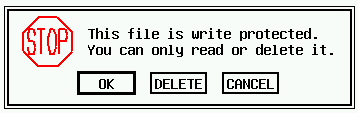
\includegraphics[width=0.5\textwidth]{alert1.eps}
\caption{A message box.}
\label{alert1}
\end{SCfigure}

Fig.~\ref{alert1} shows a typical messagebox. 
The command which produces it is:
\begin{mdframed}[hidealllines=true,backgroundcolor=blue!20]
\begin{verbatim}
ALERT 3,"This file is write protected.|You can only read or \
         delete it.",1,"OK|DELETE|CANCEL",sel
\end{verbatim}
\end{mdframed}

ALERT boxes can also be used to manage simple input forms 
like the one you can see in fig.~\ref{alert3}. 
Here is a little example program:
\begin{mdframed}[hidealllines=true,backgroundcolor=blue!20]
\begin{verbatim}
CLEARW 
i=1
name$="TEST01"
posx$="N54�50'32.3"
posy$="E007�50'32.3"
t$="Edit waypoint:||Name:   "+CHR$(27)+name$+"|"
t$=t$+"Breite: "+chr$(27)+posx$+"|"
t$=t$+"L�nge:  "+chr$(27)+posy$+"|"
t$=t$+"H�he:   "+chr$(27)+str$(alt,5,5)+"|"
t$=t$+"Typ:    "+chr$(27)+hex$(styp,4,4)+"|" 
ALERT 0,t$,1,"OK|UPDATE|L�SCHEN|CANCEL",a,f$
WHILE LEN(f$)
  WORT_SEP f$,CHR$(13),0,a$,f$
  PRINT "Feld";i;": ",a$
  INC i
WEND
QUIT
\end{verbatim}
\end{mdframed}

\begin{SCfigure}
  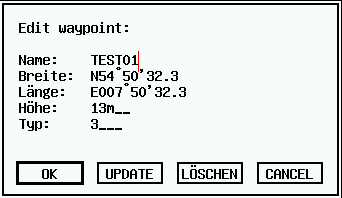
\includegraphics[width=0.5\textwidth]{alert3.eps}
  \caption{A simple input box.}
  \label{alert3}
\end{SCfigure}


\begin{SCfigure}
  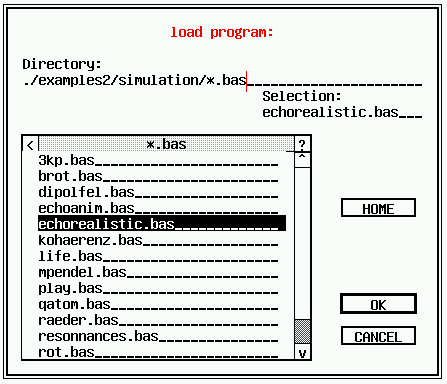
\includegraphics[width=0.7\textwidth]{fileselect.eps}
  \caption{The fileselecetor}
  \label{filesel}
\end{SCfigure}
Fig.~\ref{filesel} shows the fileselector box. The command which produces it is:
\begin{mdframed}[hidealllines=true,backgroundcolor=blue!20]
\begin{verbatim}
FILESELECT "load program:","./*.bas","in.bas",f$
\end{verbatim}
\end{mdframed}

The complete path and filename of the selected file will be returned in 
\verb|f$|.


\begin{SCfigure}
  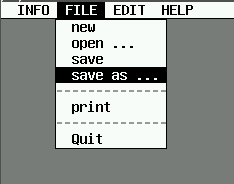
\includegraphics[width=0.3\textwidth]{menu.eps}
  \caption{A pull down menu}
  \label{filesel}
\end{SCfigure}


\section{Resources}

X11-Basic resources consist of object trees, strings, and bitmaps used by a
basic program. They encapsulate the user interface and make internationalization
easier by placing all program strings in a single file. The data format of
X11Basic resource is downwards compatible with the Atari-ST GEM implementation.

\begin{figure}
\begin{center}

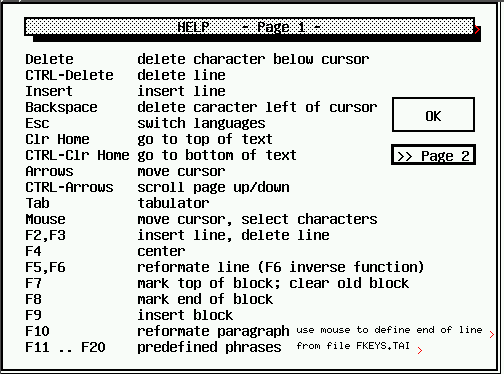
\includegraphics[width=0.48\textwidth]{form1.eps}
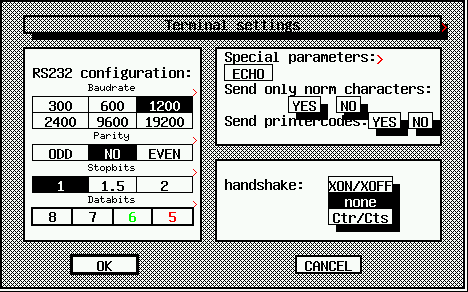
\includegraphics[width=0.48\textwidth]{form2.eps}
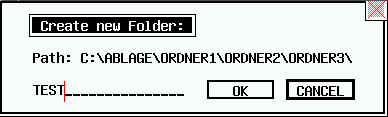
\includegraphics[width=0.48\textwidth]{form3.eps}
\end{center}
\caption{Examples of forms in X11-Basic}
\label{form1}
\end{figure}



Resources are generally created using a Resource Construction
Set (RCS) and saved to a \verb|.RSC| file which is loaded by 
\verb|RSRC_LOAD()| at program initialization time.

Resources may also be embedded as data structures in source code (the 
utility programs \verb|rsc2gui.bas| and \verb|gui2bas.bas| convert \verb|.RSC| files to 
source code). 
Resources contain pointers and coordinates which must be fixed up
before being used.
\verb|RSRC_LOAD()| does this automatically, however if you use an embedded
resource you must take care of this by yourself on each object in each object
tree to convert the initial character coordinates of to screen coordinates.
This allows resources designed on screens with different aspect ratios and
system fonts to appear the same. 
Once a resource is loaded use \verb|rsrc_gaddr()| to obtain pointers to
individual object trees which can then be manipulated directly or with the 
X11-Basic built-in functions. 

\subsection{Objects}

Objects can be boxes, buttons, text, images, and more. An object tree
is an array of OBJECT structures linked to form a structured
relationship to each other. The object itself is a section of data 
which can be held by a string in X11-Basic.

The OBJECT structure is format is as follows:

\begin{verbatim}
object$=MKI$(ob_next)+MKI$(ob_head)+MKI$(ob_tail)+
        MKI$(ob_type)+MKI$(ob_flags)+MKI$(ob_state)+
        MKL$(ob_spec)+MKI$(ob_x)+MKI$(ob_y)+MKI$(ob_width)+
        MKI$(ob_height)
\end{verbatim}

An Object tree is a collection of objects:

\begin{verbatim}
tree$=object0$+object1$+ ... +objectn$
\end{verbatim}

The first object in an OBJECT tree is called the ROOT object (OBJECT 0). It's
coordinates are relative to the upper-left hand corner of the graphics window. 
The ROOT object can have any number of children and each child can have
children of their own. In each case, the OBJECT's coordinates, \verb|ob_x|,
\verb|ob_y|, \verb|ob_width|, and \verb|ob_height| are relative to that of its
parent. The X11-Basic function \verb|objc_offset()| can, however, be used to
determine the exact screen coordinates of a child object. \verb|objc_find()| is
used to determine the object at a given screen coordinate.

The \verb|ob_next|, \verb|ob_head|, and \verb|ob_tail| fields determine this
relationship between parent OBJECTs and child OBJECTs.

\begin{description}

\item[ob\_next] the index (counting objects from the first object in the
object tree) of the object's next sibling at the same level in the object tree
array. The ROOT object should set this value to -1. The last child at any given
nesting level should set this to the index of its parent.

\item[ob\_head] the index of the first child of the current object. If the
object has no children then this value should be -1. 

\item[ob\_tail] the index of the last child: the tail of the list of the
object's children in the object tree array If the object has no children then
this value should be -1.

\item[ob\_type] the object type. The low byte of the ob\_type field 
specifies the object type as follows:

\begin{center}\begin{longtable}{|cll|}
\hline
{\bf ob\_type} & {\bf Name} & {\bf Description}\\
\hline
  20 &  G\_BOX	    &   Box		\\	    
  21 &  G\_TEXT	    &   Formatted Text  \\	    
  22 &  G\_BOXTEXT   &   Formatted Text in a Box \\
  23 &  G\_IMAGE     &   Monochrome Image	\\    
  24 &  G\_PROGDEF   &   Programmer-Defined Object\\
  25 &  G\_IBOX	    &   Invisible Box		  \\  
  26 &  G\_BUTTON    &   Push Button w/String	   \\ 
  27 &  G\_BOXCHAR   &   Character in a Box	   \\ 
  28 &  G\_STRING    &   Un-formatted Text	   \\ 
  29 &  G\_FTEXT     &   Editable Formatted Text \\
  30 &  G\_FBOXTEXT  &   Editable Formatted Text in a Box\\
  31 &  G\_ICON	    &   Monochrome Icon \\
  32 &  G\_TITLE     &   Menu Title\\
  33 &  G\_CICON     &   Color Icon \\
\hline
\end{longtable}\end{center}

\item[ob\_flags] The ob\_flags field of the object structure is a bitmask of
different flags that can be applied to any object. You may want to apply 
one ore more flags at once. Just add the values ob\_flags.

\begin{center}\begin{longtable}{|clp{9cm}|}
\hline
{\bf ob\_flags} & {\bf Name} & {\bf Description}\\
\hline
0 & NONE       & No flag \\\hline
1 & SELECTABLE & object is selected. state may be toggled by clicking on it with the mouse.\\\hline
2 & DEFAULT    & An EXIT object with this bit set will have a thicker outline and be triggered when the 
                 user presses return.\\\hline
4 & EXIT       & Clicking on this OBJECT and releasing the mouse button while still over it 
                 will cause the dialog to exit.\\\hline
8 & EDITABLE   & Set for FTEXT and FBOXTEXT objects to indicate that they may receive edit focus.\\\hline
16 & RBUTTON   & This object is one of a group of radio buttons. Clicking on it will deselect
                 any selected objects at the same tree level that also have the RBUTTON flag
                 set. Likewise, it will be deselected automatically when any other object is selected.\\\hline
32 & LASTOB    & This flag signals that the current OBJECT is the last in the object tree. (Required!)\\\hline
64 & TOUCHEXIT & Setting this flag causes the OBJECT to return an exit state immediately after   
                 being clicked on with the mouse.\\\hline
256 & HIDETREE & This OBJECT and all of its children will not be drawn.\\\hline
512 & INDIRECT & This flag cause the ob\_spec field to be interpreted as a pointer to the      
                 ob\_spec value rather than the value itself.\\\hline
1024 & FL3DIND & Setting this flag causes the OBJECT to be drawn as a 3D indicator. This is  
                 appropriate for radio and toggle buttons.\\\hline
2048 & FL3DACT & Setting this flag causes the OBJECT to be drawn as a 3D activator. This is  
                 appropriate for EXIT buttons.\\\hline
3072 & FL3DBAK & If these bits are set, the object is treated as an AES background object.  
                 If it is OUTLINED, the outlined is drawn in a 3D manner. If its color
                 is set to WHITE and its fill pattern is set to 0 then the OBJECT will inherit 
                 the default 3D background color.\\\hline
4096 & SUBMENU & This bit is set on menu items which have a sub-menu attachment. This bit also
                 indicates that the high byte of the ob\_type field is being used by the menu
                 system.\\\hline
\end{longtable}\end{center}

\item[ob\_state] The ob\_state field determines the display state of the object as
follows:

\begin{center}\begin{longtable}{|clp{9cm}|}
\hline
{\bf ob\_state} & {\bf Name} & {\bf Description}\\
\hline
0 & NORMAL   & Normal state \\\hline
1 & SELECTED & The object is selected. An object with this bit set will be drawn in inverse
               video except for G\_CICON which will use its 'selected' image.\\\hline
2 & CROSSED  & An OBJECT with this bit set will be drawn over with a white cross (this   
               state can only usually be seen over a colored or	SELECTED object).\\\hline
4 & CHECKED  & An OBJECT with this bit set will be displayed with a check mark in its    
               upper-left corner.\\\hline
8 & DISABLED & An OBJECT with this bit set will ignore user input. Text objects with this   
               bit set will draw in grey or a dithered pattern.\\\hline
16 & OUTLINED & G\_BOX, G\_IBOX, G\_BOXTEXT, G\_FBOXTEXT, and G\_BOXCHAR OBJECTs   
               with this bit set will be drawn with a double border.\\\hline
32 & SHADOWED & G\_BOX, G\_IBOX, G\_BOXTEXT, G\_FBOXTEXT, and G\_BOXCHAR OBJECTs   
                will be drawn with a shadow.\\\hline
\end{longtable}\end{center}

\item[ob\_spec] The Object-Specific Field

The ob\_spec field contains different data depending on the object type
as indicated in the table below:
\begin{center}\begin{longtable}{|lp{9cm}|}
\hline
G\_BOX &
The low 16 bits contain a WORD containing color information for the OBJECT. 
Bits 23-16 contain a signed BYTE representing the border thickness of the 
box.\\\hline
G\_TEXT &The ob\_spec field contains a pointer to a TEDINFO  structure. \\\hline  
G\_BOXTEXT &The ob\_spec field contains a pointer to a TEDINFO structure.   \\\hline
G\_IMAGE   & The ob\_spec field points to a BITBLK structure. \\\hline
G\_PROGDEF & The ob\_spec field points to a APPLBLK structure.\\\hline
G\_IBOX	  & The low 16 bits contain a WORD containing color information for the OBJECT. 
Bits 23-16 contain a signed BYTE representing the border thickness of the box.\\\hline
G\_BUTTON  & The ob\_spec field contains a pointer to the text to be contained in the button.\\\hline
G\_BOXCHAR & The low 16 bits contain a WORD containing color information for the OBJECT. 
Bits 23-16 contain a signed BYTE representing the border thickness of the box. 
Bits 31-24 contain the ASCII value of the character to display.\\\hline
G\_STRING  & The ob\_spec field contains a pointer to the text to be displayed.\\\hline
G\_FTEXT   & The ob\_spec field contains a pointer to a TEDINFO structure.\\\hline
G\_FBOXTEXT & The ob\_spec field contains a pointer to a TEDINFO structure.\\\hline
G\_ICON & The ob\_spec field contains a pointer to an ICONBLK structure. \\\hline    
G\_TITLE  & The ob\_spec field contains a pointer to the text to be used for the title.\\\hline
G\_CICON  & The ob\_spec field contains a pointer to a CICONBLK structure.\\\hline
\end{longtable}\end{center}

\begin{description}
\item[objc\_colorword]
Almost all objects reference a WORD containing the object color as
defined below.

{\footnotesize
\begin{verbatim}
objc_colorword=bbbbcccctpppcccc

Bits 15-12 contain the border color 
Bits 11-8  contain the text color 
Bit   7    is 1 if opaque or 0 if transparent 
Bits 6-4   contain the fill pattern index 
Bits 3-0   contain the fill color 
\end{verbatim}}

Available colors for fill patterns, text, and borders are listed
below:
\begin{center}
\begin{tabular}{|cll|}
\hline
{\bf Value} &{\bf  Name}&{\bf  Color}  \\
\hline
 0&  WHITE	&  White\\
 1&  BLACK	&  Black\\
 2&  RED	&  Red\\
 3&  GREEN	&  Green\\
 4&  BLUE	&  Blue\\
 5&  CYAN	&  Cyan\\
 6&  YELLOW	&  Yellow\\
 7&  MAGENTA	&  Magenta\\
 8&  LWHITE	&  Light Gray\\
 9&  LBLACK	&  Dark Gray\\
 10& LRED	&  Light Red\\
 11& LGREEN	&  Light Green\\
 12& LBLUE	&  Light Blue\\
 13& LCYAN	&  Light Cyan\\
 14& LYELLOW	&  Light Yellow\\
 15& LMAGENTA	&  Light Magenta\\
\hline
\end{tabular}
\end{center}


\item[TEDINFO]
G\_TEXT, G\_BOXTEXT, G\_FTEXT, and G\_FBOXTEXT objects all reference a
TEDINFO structure in their ob\_spec field. The TEDINFO structure is
defined below:
 {\footnotesize
\begin{verbatim}                                                         
tedinfo$=MKL$(VARPTR(te_ptext$))+MKL$(VARPTR(te_ptmplt$))+
         MKL$(VARPTR(te_pvalid$))+MKI$(te_font)+MKI$(te_fontid)+
         MKI$(te_just)+MKI$(te_color)+MKI$(te_fontsize)+
         MKI$(te_thickness)+MKI$(te_txtlen)+MKI$(te_tmplen)
\end{verbatim}}

The three character pointer point to text strings required for 
\verb|G_FTEXT|
and \verb|G_FBOXTEXT| objects. te\_ptext points to the actual text to be
displayed and is the only field used by all text objects. te\_ptmplt
points to the text template for editable fields. For each character
that the user can enter, the text string should contain a tilde
character (ASCII 126). Other characters are displayed but cannot be
overwritten by the user. \verb|te_pvalid| contains validation characters for
each character the user may enter. The current acceptable validation
characters are:

\begin{center}
\begin{tabular}{|cl|}
\hline
{\bf Character} &{\bf  Allows}\\
\hline
9 & Digits 0-9\\
A & Uppercase letters A-Z plus space\\
a & Upper and lowercase letters plus space\\
N & Digits 0-9, uppercase letters A-Z and space\\
n & Digits 0-9, upper and lowercase letters A-Z  and space\\
F & Valid DOS filename characters plus question mark and asterisk \\
P & Valid DOS pathname characters, backslash, colon, question mark, asterisk \\
p & Valid DOS pathname characters, backslash and colon\\
X & All characters\\
\hline
\end{tabular}
\end{center}

\verb|te_font| may be set to any of the following values:

\begin{center}
\begin{tabular}{|cll|}
\hline
{\bf te\_font} &{\bf  Name} & {\bf Description} \\
\hline
3 &IBM    & Use the standard monospaced font.\\
5 &SMALL  &  Use the small monospaced font.\\
\hline
\end{tabular}
\end{center}

\verb|te_just| sets the justification of the text output as follows:

\begin{center}
\begin{tabular}{|cll|}
\hline
{\bf te\_just} &{\bf  Name} & {\bf Description} \\
\hline
0 & TE\_LEFT & Left Justify\\
1 & TE\_RIGHT & Right Justify\\
2 & TE\_CNTR & Center\\
\hline
\end{tabular}
\end{center}


te\_thickness sets the border thickness (positive and negative values
are acceptable) of the G\_BOXTEXT or G\_FBOXTEXT object. 

te\_txtlen and
te\_tmplen should be set to the length of the starting text and
template length respectively. 

\item[BITBLK]
G\_IMAGE objects contain a pointer to a BITBLK structure in their
ob\_spec field. The BITBLK structure is defined as follows:

 {\footnotesize
\begin{verbatim}                                                         
bitblk$=MKL$(VARPTR(bi_pdata$))+MKI$(bi_wb)+MKI$(bi_hl)+
        MKI$(bi_x)+MKI$(bi_y)+MKI$(bi_color)
\end{verbatim}}

\verb|bi_pdata| should contain a monochrome bit image. 
\verb|bi_wb| specifies the width (in bytes) of the image. 
All BITBLK images must be a multiple of 16 pixels wide therefore this 
value must be even.
\verb|bi_hl| specifies the height of the image in scan lines (rows). 
\verb|bi_x| and \verb|bi_y| are used as offsets into \verb|bi_pdata|. 
Any data occurring before these coordinates will be ignored. 
\verb|bi_color| is a standard color WORD
where the fill color specifies the color in which the image will be
rendered.

\item[ICONBLK]
The \verb|ob_spec| field of \verb|G_ICON| objects point to an ICONBLK structure as
defined below:

 {\footnotesize
\begin{verbatim}                                                         
iconblk$=MKL$(VARPTR(ib_pmask$))+MKL$(VARPTR(ib_pdata$))+MKL$(VARPTR(ib_ptext$))+
         MKI$(ib_char)+MKI$(ib_xchar)+MKI$(ib_ychar)+
         MKI$(ib_xicon)+MKI$(ib_yicon)+MKI$(ib_wicon)+MKI$(ib_hicon)+
	 MKI$(ib_xtext)+MKI$(ib_ytext)+MKI$(ib_wtext)+MKI$(ib_htext)
\end{verbatim}}

\verb|ib_pmask| and \verb|ib_pdata| contain the monochrome mask and 
image data respectively. \verb|ib_ptext| is a string pointer to the icon text.
\verb|ib_char| defines the icon character (used for drive icons) and the icon
foreground and background color as follows:

 {\footnotesize
\begin{verbatim}                                                         
|                              ib_char                               |
|      Bits 15-12      |      Bits 11-8       |       Bits 7-0       |
|Icon Foreground Color |Icon Background Color |ASCII Character (or 0 |
|                      |                      |  for no character).  |
\end{verbatim}}

\verb|ib_xchar| and \verb|ib_ychar| specify the location of the icon character
relative to \verb|ib_xicon| and \verb|ib_yicon|. \verb|ib_xicon| and 
\verb|ib_yicon| specify the
location of the icon relative to the \verb|ob_x| and \verb|ob_y| of the object.
\verb|ib_wicon| and \verb|ib_hicon| specify the width and height of the icon in
pixels. As with images, icons must be a multiple of 16 pixels in
width.
\verb|ib_xtext| and \verb|ib_ytext| specify the location of the text string relative
to the \verb|ob_x| and \verb|ob_y| of the object. \verb|ib_wtext| and \verb|ib_htext| specify the
width and height of the icon text area.

\item[CICONBLK]

The \verb|G_CICON| object defines its
\verb|ob_spec| field to be a pointer to a CICONBLK structure as defined
below:

 {\footnotesize
\begin{verbatim}                                                         
ciconblk$=monoblk$+MKL$(VARPTR(mainlist$))
\end{verbatim}}

\verb|monoblk| contains a monochrome icon which is rendered if a color icon
matching the display parameters cannot be found. In addition, the icon
text, character, size, and positioning data from the monochrome icon
are always used for the color one. \verb|mainlist| contains the first
CICON structure in a linked list of color icons for different
resolutions. \verb|CICON| is defined as follows:

 {\footnotesize
\begin{verbatim}                                                         
cicon$=MKI$(num_planes)+MKL$(VARPTR(col_data$))+MKL$(VARPTR(col_mask$))+
       MKL$(VARPTR(sel_data$))+MKL$(VARPTR(sel_mask$))+
       MKL$(VARPTR(cicon2$))
\end{verbatim}}

\verb|num_planes| indicates the number of bit planes this color icon
contains. \verb|col_data| and \verb|col_mask| contain the icon data and 
mask for the unselected icon respectively. Likewise, 
\verb|sel_data| and \verb|sel_mask| contain the icon data and mask for 
the selected icon. \verb|cicon2$| contains
the next color icon definition. Use \verb|MKL$(0)| if no more are available.

The GUI library searches the CICONBLK object for a color icon that has the
same number of planes in the display. If none is found, the GUI library simply
uses the monochrome icon.

\item[APPLBLK]

\verb|G_PROGDEF| objects allow programmers to define custom objects and link
them transparently in the resource. The \verb|ob_spec| field of
\verb|G_PROGDEF|
objects contains a pointer to an APPLBLK as defined below:

 {\footnotesize
\begin{verbatim}                                                         
applblk$=MKL$(SYM_ADR(#1,"function"))+MKL$(ap_parm)
\end{verbatim}}

The first is a pointer to a user-defined routine which will draw the
object. This routine must be a c-Function, which has to be linked to 
X11-basic with the LINK command. The routine will be passed a pointer to a
PARMBLK structure containing the information it needs to render the
object. The routine must be defined with stack checking off and expect
to be passed its parameter on the stack. \verb|ap_parm| is a user-defined
value which is copied into the PARMBLK structure as defined below:

{\footnotesize
\begin{verbatim}                                                         
typedef struct parm_blk {
        OBJECT          *tree;
        short            pb_obj;
        short            pb_prevstate;
        short            pb_currstate;
        short            pb_x;
        short            pb_y;
        short            pb_w;
        short            pb_h;
        short            pb_xc;
        short            pb_yc;
        short            pb_wc;
        short            pb_hc;
        long             pb_parm;
} PARMBLK;
\end{verbatim}}

\verb|tree| points to the OBJECT tree of the object being drawn. The object
is located at index \verb|pb_obj|.

The routine is passed the old \verb|ob_state| of the object in
\verb|pb_prevstate|
and the new \verb|ob_state| of the object in \verb|pb_currstate|. 
If \verb|pb_prevstate|
and \verb|pb_currstate| is equal then the object should be drawn completely,
otherwise only the drawing necessary to redraw the object from
\verb|pb_prevstate| to \verb|pb_currstate| are necessary.

\verb|pb_x|, \verb|pb_y|, \verb|pb_w|, and \verb|pb_h| give the screen 
coordinates of the object.
\verb|pb_xc|, \verb|pb_yc|, \verb|pb_wc|, and \verb|pb_hc| give the 
rectangle to clip to. \verb|pb_parm|
contains a copy of the \verb|ap_parm| value in the APPLBLK structure.
The custom routine should return a short containing any remaining
\verb|ob_state| bits you wish the GUI Library to draw over your custom object.

\end{description}

\end{description}



\subsubsection{Dialogs}

Dialog boxes are modal forms of user input. This means that no other
interaction can occur between the user and applications until the
requirements of the dialog have been met and it is exited. A normal
dialog box consists of an object tree with a BOX
as its root object and any number of other controls that accept user
input. Both alert boxes and the file selector are examples of
dialog boxes.

The \verb|form_do()| function performs the simplest method of using a dialog box. Simply
construct an OBJECT tree with at least one EXIT or TOUCHEXIT object and call
\verb|form_do()|\footnote{Before you should display the dialog box using the
{\tt objc\_draw()} function. Maybe you also want to center the dialog with 
{\tt form\_center()} and save and redraw the background 
with {\tt form\_dial()}.}. All interaction with the dialog like editable fields,
radio buttons, and selectable objects will be maintained by the 
X11-Basic library until the
user strikes an EXIT or TOUCHEXIT object.


\subsection{The gui file format}

The *.gui file format, which is basically an ASCII representation of the ATARI
ST resource files (*.rsc), can be converted to X11-Basic code, which then can
handle message boxes and forms. The converter \verb|gui2bas(1)| does this job.
For conversion of ATARI ST resource files to *.gui Files see \verb|rsc2gui(1)|.

The *.gui file consists of Lines and Blocks which specify objects and their 
hierarchical dependencies.
The generic format of such an object is:

\begin{verbatim}
label: TYPE(variables) {
 ... block ...
}
\end{verbatim}

The label is optional and gives the object a name. Depending on TYPE of the
object, one or more variables are given as a comma separated list in
brackets. 

Each object may start a block with '\{' at the end of the line. Inside this
block there might be one or more objects given which then are considered as
sub-objects of the one which opened the block. The block will be closed by a
'\}' in a single line.

\begin{mdframed}[hidealllines=true,backgroundcolor=green!20]

Example:

{\footnotesize\linespread{0.8}
\begin{verbatim}
' Little selector box  (c) Markus Hoffmann    07.2003
' convert this with gui2bas !
' as an example for the use of the gui system
' with X11-Basic

BOX(X=0,Y=0,W=74,H=14, FRAME=2, FRAMECOL=1, TEXTCOL=1, BGCOL=0, PATTERN=0, TEXTMODE=0, STATE=OUTLINED+) {
  BOXTEXT(X=2,Y=1,W=70,H=1, TEXT="Select option ...", FONT=3, JUST=2, COLOR=4513, BORDER=253, STATE=SHADOWED+)
  BOX(X=2,Y=3,W=60,H=10, FRAME=-1, FRAMECOL=1, TEXTCOL=1, BGCOL=0, PATTERN=0, TEXTMODE=0) {
    FTEXT(X=1,Y=1,W=30,H=1,COLOR=4513,FONT=3,BORDER=1,TEXT="Line 1", PTMP="_______________________________________",PVALID="XXXXXXXXXXXXXXXXXXXXXXXXXXXXXXXXXXXXXXX", FLAGS=EDITABLE)
    FTEXT(X=1,Y=2,W=30,H=1,COLOR=4513,FONT=3,BORDER=1,TEXT="", PTMP="_______________________________________",PVALID="XXXXXXXXXXXXXXXXXXXXXXXXXXXXXXXXXXXXXXX", FLAGS=EDITABLE)
    FTEXT(X=1,Y=3,W=30,H=1,COLOR=4513,FONT=3,BORDER=1,TEXT="", PTMP="_______________________________________",PVALID="XXXXXXXXXXXXXXXXXXXXXXXXXXXXXXXXXXXXXXX", FLAGS=EDITABLE)
    FTEXT(X=1,Y=4,W=30,H=1,COLOR=4513,FONT=3,BORDER=1,TEXT="", PTMP="_______________________________________",PVALID="XXXXXXXXXXXXXXXXXXXXXXXXXXXXXXXXXXXXXXX", FLAGS=EDITABLE)
    BOX(X=2,Y=6,W=50,H=3, FRAME=-1, FRAMECOL=1, TEXTCOL=1, BGCOL=1, PATTERN=5, TEXTMODE=0) { 
      BUTTON(X=2,Y=1,W=4,H=1, TEXT="ON",STATE=SELECTED, FLAGS=RADIOBUTTON+SELECTABLE,FRAME=2, FRAMECOL=1, TEXTCOL=1, BGCOL=1, PATTERN=0, TEXTMODE=0)
      BUTTON(X=8,Y=1,W=4,H=1, TEXT="OFF",FLAGS=RADIOBUTTON+SELECTABLE,FRAME=2, FRAMECOL=1, TEXTCOL=1, BGCOL=1, PATTERN=0, TEXTMODE=0)
    }
  }
  ok:	  BUTTON(X=65,Y=4,W=7,H=4, TEXT="OK", FLAGS=SELECTABLE+DEFAULT+EXIT)
  cancel: BUTTON(X=65,Y=9,W=7,H=4, TEXT="CANCEL", FLAGS=SELECTABLE+EXIT+LASTOB+)
}
\end{verbatim}
}
\end{mdframed}

\section{Menus}

Most applications use a menu bar to allow the user to navigate through program
options. In addition, future versions of X11-Basic will allow pop-up menus and
drop-down list boxes (a special form of a pop-up menu). 

Here is a simple example program, which demonstrates the handling of a drop
down menu. 

\begin{mdframed}[hidealllines=true,backgroundcolor=blue!20]
{\footnotesize\linespread{0.8}
\begin{verbatim}
' Test-program for Drop-Down-Menus
'
DIM field$(50)
FOR i=0 TO 50
  READ field$(i)
  EXIT IF field$(i)="***"
NEXT i
oh=0
field$(i)=""
DATA "INFO","  Menutest"
DATA "---------------"
DATA "- Access.1","- Access.2","- Access.3","- Access.4","- Access.5"
DATA "- Access.6",""
DATA "FILE","  new","  open ...","  save","  save as ...","--------------"
DATA "  print","--------------","  Quit",""
DATA "EDIT","  cut","  copy","  paste","----------","  help1","  helper"
DATA "  assist",""
DATA "HELP","  online help","--------------","  edifac","  editor","  edilink"
DATA "  edouard",""
DATA "***"

grau=get_color(32000,32000,32000)
color grau
pbox 0,0,640,400
MENUDEF field$(),menuaction
DO 
  pause 0.05
  MENU 
LOOP
quit

PROCEDURE menuaction(k)
  local b
  IF (field$(k)="  Quit") OR (field$(k)="  exit") 
    quit
  ELSE IF field$(k)="  online help"
    oh=not oh
    MENUSET k,4*abs(oh)
  ELSE IF field$(k)="  Menutest" 
    ~form_alert(1,"[0][---- Menutest ----||(c) Markus Hoffmann 2001|X11-Basic V.1.03][ OK ]")
  ELSE   
    PRINT "MENU selected ";k;" contents: ";field$(k)
    b=form_alert(1,"[1][--- Menutest ---||You selected item (No. "+str$(k)+"),| for which was no|function defined !][ OK |disable]")
    if b=2
      MENUSET k,8
    endif
  ENDIF
RETURN
\end{verbatim}
}
\end{mdframed}


\chapter{WEB Programming}

This chapter explains how you can use X11-Basic programs for WEB-interfacing.
Especially via the use of so-called {\bf CGI-Scripts}.  

\section{What is CGI?}

CGI stands for {\em Common Gateway Interface} --- a term you don't really need to
know. In short, CGI defines how web servers and web browsers handle information
from HTML forms on web pages. This means instead of the WEB server sending
static  web pages to the clients, it can invoke a program, typically called a
cgi-script,  to generate the page on the time the request was received. These
cgi-scripts take some action, and then send a results page back to the user's
web browser. The results page might be different every time the program is run.

And these programs can be X11-Basic programs.

\subsection{Configuration}
\begin{enumerate}
\item {\bf All X11-Basic scripts must begin} with the following statement, on the first 
line:
\begin{mdframed}[hidealllines=true,backgroundcolor=blue!20]
\begin{verbatim}
#!/usr/bin/xbasic
\end{verbatim}
\end{mdframed}

Because Unix does not map file suffixes to programs, there has to be a way to 
tell Unix that this file is a X11-Basic program, and that it is to be executed
by the X11-Basic interpreter \verb|xbasic|. This is seen before in shell
scripts, in which the first line tells Unix to execute it with one of the shell
programs. The xbasic executable, which will take this file, parse it, and
execute it, is located in the directory /usr/bin. This may be different on some
systems. If you are not sure where the xbasic executable is, type which xbasic
on the command line, and it will return you the path.

\item {\bf All scripts should be marked as executable by the system.}

Executable files are types that contain instructions for the machine or an
interpreter, such as xbasic, to execute. To mark a file as executable, you need
to alter the file permissions on the script file. There are three basic
permissions: read, write, and execute. There are also three levels of access:
owner, group, and anyone. X11-Basic files should have their permissions changed so
that you, the owner, has permission to read, write and execute your file, while
others only have permission to read and execute your file. This is done with
the following command:


\begin{mdframed}[hidealllines=true,backgroundcolor=black!20]
\begin{verbatim}
chmod 755 filename.bas
\end{verbatim}
\end{mdframed}


The number 755 is the file access mask. The first digit is your permission; it
is 7 for full access. The user and anyone settings are 5 for read and execute.

\item {\bf The very first print statement} in a X11-Basic cgi script that
returns HTML should be:

\begin{mdframed}[hidealllines=true,backgroundcolor=blue!20]
\begin{verbatim}
PRINT "Content-type: text/html"+CHR$(13)
PRINT ""+CHR$(13)
FLUSH
\end{verbatim}
\end{mdframed}

When your X11-Basic script is going to return an HTML file, you must have this
as the very first print statement in order to tell the web server that this is
an HTML file. There must be two end of line characters (CR+LF) (the additional
\verb|chr$(13)|) in order for this to work. The flush statement ensures, that
this statement is sent to the web-server. After that, you usually 
\verb|print "<HTML><BODY>"| etc.

\item {\bf End your program with \verb|quit|}

Do not use \verb|END|. Otherwise the cgi-program will remain is the servers 
memory as a zombie.

\item {\bf Always use the POST method with HTML forms}

There are 2 ways to get information from the client to the web server. The GET
method takes all of the data from the forms and concatenates it onto the end of
the URL. This information is then passed to the CGI program as an environment 
variable (\verb|QUERY_STRING|). Because the GET method has the limitation of being 1024 characters
long, it is best to use the POST method. This takes the data and sends it
along with the request to the web server, without the user seeing the ugly
strings in the URL. This information is passed to the CGI program through
standard in, which the program can easily read from. To use the POST method,
make sure that your HTML form tag has \verb|METHOD=POST| (no quotes).

\item {\bf HTML forms must reference the cgi script to be executed.}

In your FORM tag, there is an ACTION attribute. This is like the HREF attribute
for a link. It should be the URL of the CGI program you want the form data sent
to. Usually this is
\verb|ACTION="/cgi-bin/filename.bas"|

\item {\bf X11-Basic-cgi files usually go in the cgi-bin directory of your web server.}

The web server has a "root" directory. This is the highest directory your HTML
files can access. (You don't want clients to be able to snoop around your
entire system, so the rest of the system is sealed off) in
this directory, there is usually one called cgi-bin, where all the CGI programs
go. Some web service providers give each user a cgi-local directory in their
home directory where they can put their cgi scripts. If this is the case, use
this one instead. 
\end{enumerate}

\section{How it works}\index{CGI|bb}

When a user activates a link to a gateway script, input is sent to the server.
The server formats this data into environment variables and checks to see
whether additional data was submitted via the standard input stream.

\subsection{Environment Variables}\index{Environment Variables}

Input to CGI scripts is usually in the form of environment variables. The
environment variables passed to gateway scripts are associated with the browser
requesting information from the server, the server processing the request, and
the data passed in the request. Environment variables are case-sensitive and are
normally used as described in this section. The standard (and platform
independent) environment variables are shown in the following table:

\begin{center}
\begin{longtable}{|l|p{10cm}|}
\hline
{\bf Variable} & {\bf Purpose}\\
\hline
\verb|AUTH_TYPE| & 
Specifies the authentication method and is used to validate a user's access.
\\\hline
\verb|CONTENT_LENGTH| & Used to provide a way of tracking the length of the 
data string as a numeric value.\\\hline
\verb|CONTENT_TYPE| & Indicates the MIME type of data. \\\hline
\verb|GATEWAY_INTERFACE| & Indicates which version of the CGI standard the 
server is using.\\\hline
\verb|HTTP_ACCEPT|	& Indicates the MIME content types the browser will accept, 
as passed to the gateway script via the server.\\\hline
\verb|HTTP_USER_AGENT| & Indicates the type of browser used to send the request, 
as passed to the gateway script via the server.\\\hline
\verb|PATH_INFO| & Identifies the extra information included in the URL after 
the identification of the CGI script. \\\hline
\verb|PATH_TRANSLATED| & Set by the server based on the PATH\_INFO variable. 
The server translates the PATH\_INFO variable into this variable. \\\hline
\verb|QUERY_STRING| & Set to the query string (if the URL contains a query string).\\\hline 
\verb|REMOTE_ADDR| & Identifies the Internet Protocol address of the remote computer making the request.\\\hline 
\verb|REMOTE_HOST| & Identifies the name of the machine making the request.\\\hline 
\verb|REMOTE_IDENT| & Identifies the machine making the request.\\\hline 
\verb|REMOTE_USER| & Identifies the user name as authenticated by the user.\\\hline 
\verb|REQUEST_METHOD| & Indicates the method by which the request was made. \\\hline 
\verb|SCRIPT_NAME| & Identifies the virtual path to the script being executed.\\\hline 
\verb|SERVER_NAME| & Identifies the server by its host name, alias, or IP address.\\\hline 
\verb|SERVER_PORT| & Identifies the port number the server received the request on.\\\hline
\verb|SERVER_PROTOCOL| & Indicates the protocol of the request sent to the server.\\\hline
%\verb|SERVER_SOFTWARE| & Identifies the Web server software.\\\hline
\end{longtable}
\end{center}
\begin{description}

\item[AUTH\_TYPE]

The \verb|AUTH_TYPE| variable provides access control to protected areas of
the Web server and can be used only on servers that support user
authentication. If an area of the Web site has no access control, the
\verb|AUTH_TYPE| variable has no value associated with it. If an area of the
Web site has access control, the \verb|AUTH_TYPE| variable is set to a specific
value that identifies the authentication scheme being used. e.g. "Basic".

Using this mechanism, the server can challenge a client's request and the
client can respond. To do this, the server sets a value for the
\verb|AUTH_TYPE| variable and the client supplies a matching value. The next
step is to authenticate the user. Using the basic authentication scheme, the
user's browser must supply authentication information that uniquely
identifies the user. This information includes a user ID and password.


\item[CONTENT\_LENGTH]

The \verb|CONTENT_LENGTH| variable provides a way of tracking the length of the
data string. This variable tells the client and server how much data to read on
the standard input stream. The value of the variable corresponds to the number
of characters in the data passed with the request. If no data is being passed,
the variable has no value.


\item[CONTENT\_TYPE]

The \verb|CONTENT_TYPE| variable indicates the data's MIME type. This
variable is set only when attached data is passed using the standard input
or output stream. The value assigned to the variable identifies the basic MIME
type and subtype as follows:
\begin{center}
\begin{longtable}{|l|p{10cm}|}
\hline
{\bf Type} & {\bf Description}\\
\hline
\verb|application| & Binary data that can be executed or used with another 
application\\\hline
\verb|audio| & A sound file that requires an output device to preview\\\hline
\verb|image| & A picture that requires an output device to preview\\\hline
\verb|message| & An encapsulated mail message\\\hline
\verb|multipart| & Data consisting of multiple parts and possibly many data 
types\\\hline
\verb|text| & Textual data that can be represented in any character set or formatting language\\\hline
\verb|video| & A video file that requires an output device to preview\\\hline
\verb|x-world|   & Experimental data type for world files\\\hline
\end{longtable}
\end{center}

MIME subtypes are defined in three categories: primary, additionally defined,
and extended. The primary subtype is the primary type of data adopted for use
as a MIME content type. Additionally defined data types are additional subtypes
that have been officially adopted as MIME content types. Extended data types
are experimental subtypes that have not been officially adopted as MIME content
types. You can easily identify extended subtypes because they begin with the
letter x followed by a hyphen. The following Table lists common MIME types and
their descriptions.
\begin{center}
\begin{longtable}{|l|p{8cm}|}
\hline
{\bf Type/Subtype} & {\bf Description}\\\hline 
\verb|application/octet-stream| & Binary data that can be executed or used with another application\\\hline 
\verb|application/pdf| & ACROBAT PDF document\\\hline 
\verb|application/postscript| & Postscript-formatted data\\\hline
\verb|application/x-compress| & Data that has been compressed using UNIX 
compress\\\hline
%\verb|application/x-dvi| & Device-independent file\\\hline 
\verb|application/x-gzip| & Data that has been compressed using UNIX gzip\\\hline
%\verb|application/x-latex| & LATEX document\\\hline
\verb|application/x-tar| & Data that has been archived using UNIX tar\\\hline
%\verb|audio/basic| & Audio in a nondescript format\\\hline
\verb|audio/x-wav| & Audio in Microsoft WAV format\\\hline
\verb|image/gif| & Image in gif format\\\hline
\verb|image/jpeg| & Image in JPEG format\\\hline
\verb|image/tiff| & Image in TIFF format\\\hline
%\verb|image/x-portable-bitmap| & Portable bitmap\\\hline
%\verb|image/x-portable-graymap| & Portable graymap\\\hline
%\verb|image/x-portable-pixmap| & Portable pixmap\\\hline
%\verb|image/x-xbitmap| & X-bitmap\\\hline
%\verb|image/x-xpixmap| & X-pixmap\\\hline
%\verb|message/external-body| & Message with external data source\\\hline
%\verb|message/partial| & Fragmented or partial message\\\hline
%\verb|message/rfc822| & RFC 822-compliant message\\\hline 
%\verb|multipart/alternative| & Data with alternative formats\\\hline
%\verb|multipart/digest| & Multipart message digest\\\hline
\verb|multipart/mixed| & Multipart message with data in multiple formats\\\hline
%\verb|multipart/parallel| & Multipart data with parts that should be viewed simultaneously\\\hline
\verb|text/html| & HTML-formatted text\\\hline
\verb|text/plain| & Plain text with no HTML formatting included\\\hline
\verb|video/mpeg| & Video in the MPEG format\\\hline
%\verb|video/x-msvideo| & Video in the Microsoft AVI format\\\hline
\end{longtable}
\end{center}
Note, that there are more than the above listed types.

Some MIME content types can be used with additional parameters. These content
types include text/plain, text/html, and all multi-part message data. The
charset parameter, which is optional, is used with the text/plain type to
identify the character set used for the data. If a charset is not specified, the
default value charset=us-ascii is assumed. Other values for charset include any
character set approved by the International Standards Organization. These
character sets are defined by ISO-8859-1 to ISO-8859-9 and are specified as
follows:

{\footnotesize
\begin{verbatim}
 CONTENT_TYPE = text/plain; charset=iso-8859-1
\end{verbatim}
}

The boundary parameter, which is required, is used with multi-part data to
identify the boundary string that separates message parts. The boundary value is
set to a string of 1 to 70 characters. Although the string cannot end in a
space, it can contain any valid letter or number and can include spaces and a
limited set of special characters. Boundary parameters are unique strings that
are defined as follows:

{\footnotesize
\begin{verbatim}
 CONTENT_TYPE = multipart/mixed; boundary=boundary_string
\end{verbatim}
}

\item[GATEWAY\_INTERFACE]

The \verb|GATEWAY_INTERFACE| variable indicates which version of the CGI
specification the server is using. The value assigned to the variable identifies
the name and version of the specification used as follows:

\begin{verbatim}
 GATEWAY_INTERFACE = name/version
\end{verbatim}

The version of the CGI specification is 1.1. A server conforming
to this version would set the \verb|GATEWAY_INTERFACE| variable as follows:

\begin{verbatim}
 GATEWAY_INTERFACE = CGI/1.1
\end{verbatim}

\item[HTTP\_ACCEPT]

The \verb|HTTP_ACCEPT| variable defines the types of data the client will
accept. The acceptable values are expressed as a type/subtype pair. Each
type/subtype pair is separated by commas.

\item[HTTP\_USER\_AGENT]

The \verb|HTTP_USER_AGENT| variable identifies the type of browser used to send
the request. The acceptable values are expressed as software type/version
or library/version. 

\item[PATH\_INFO]

The \verb|PATH_INFO| variable specifies extra path information and can be used
to send additional information to a gateway script. The extra path information
follows the URL to the gateway script referenced. Generally, this information
is a virtual or relative path to a resource that the server must interpret. 

\item[PATH\_TRANSLATED]

Servers translate the \verb|PATH_INFO| variable into the {\tt PATH\_TRANSLATED}
variable by inserting the default Web document's directory path in front of the
extra path information. 

\item[QUERY\_STRING]

The \verb|QUERY_STRING| variable specifies an URL-encoded search string. You set
this variable when you use the GET method to submit a fill-out form. The query string is
separated from the URL by a question mark. The user submits all the
information following the question mark separating the URL from the query
string. The following is an example:

\begin{verbatim}
 /cgi-bin/doit.cgi?string
\end{verbatim}

When the query string is URL-encoded, the browser encodes key parts of the
string. The plus sign is a placeholder between words and acts as a
substitute for spaces:

\begin{verbatim}
 /cgi-bin/doit.cgi?word1+word2+word3
\end{verbatim}

Equal signs separate keys assigned by the publisher from values entered by
the user. In the following example, response is the key assigned by the
publisher, and never is the value entered by the user:

\begin{verbatim}
 /cgi-bin/doit.cgi?response=never
\end{verbatim}

Ampersand symbols separate sets of keys and values. In the following
example, response is the first key assigned by the publisher, and
sometimes is the value entered by the user. The second key assigned by the
publisher is reason, and the value entered by the user is I am not really
sure:

{\footnotesize
\begin{verbatim}
 /cgi-bin/doit.cgi?response=sometimes&reason=I+am+not+really+sure
\end{verbatim}
}

Finally, the percent sign is used to identify escape characters. Following
the percent sign is an escape code for a special character expressed as a
hexadecimal value. Here is how the previous query string could be
rewritten using the escape code for an apostrophe:

{\footnotesize
\begin{verbatim}
 /cgi-bin/doit.cgi?response=sometimes&reason=I%27m+not+really+sure
\end{verbatim}
}


\item[REMOTE\_ADDR]

The \verb|REMOTE_ADDR| variable is set to the Internet Protocol (IP) address
of the remote computer making the request. 

\item[REMOTE\_HOST]

The \verb|REMOTE_HOST| variable specifies the name of the host computer making a
request. This variable is set only if the server can figure out this
information using a reverse lookup procedure. 

\item[REMOTE\_IDENT]

The \verb|REMOTE_IDENT| variable identifies the remote user making a request. The
variable is set only if the server and the remote machine making the
request support the identification protocol. Further, information on the
remote user is not always available, so you should not rely on it even
when it is available. 

\item[REMOTE\_USER]

The \verb|REMOTE_USER| variable is the user name as authenticated by the user,
and as such is the only variable you should rely upon to identify a user.
As with other types of user authentication, this variable is set only if
the server supports user authentication and if the gateway script is
protected. 

\item[REQUEST\_METHOD]

The \verb|REQUEST_METHOD| variable specifies the method by which the request
was made. The methods could be any of \verb|GET|, \verb|HEAD|, \verb|POST|,
\verb|PUT|, \verb|DELETE|, \verb|LINK| and  \verb|UNLINK|.

The \verb|GET|, \verb|HEAD| and \verb|POST| methods are the most commonly
used request methods. Both \verb|GET| and \verb|POST| are used to submit forms. 

\item[SCRIPT\_NAME]

The \verb|SCRIPT_NAME| variable specifies the virtual path to the script being
executed. This information is useful if the script generates an HTML document
that references the script.

\item[SERVER\_NAME]

The \verb|SERVER_NAME| variable identifies the server by its host name, alias,
or IP address. This variable is always set.

\item[SERVER\_PORT]

The \verb|SERVER_PORT| variable specifies the port number on which the server received
the request. This information can be interpreted from the URL to the script if
necessary. However, most servers use the default port of 80 for HTTP requests.

\item[SERVER\_PROTOCOL]

The \verb|SERVER_PROTOCOL| variable identifies the protocol used to send the
request. The value assigned to the variable identifies the name and
version of the protocol used. The format is name/version, such as
HTTP/1.0. 

%\item[SERVER\_SOFTWARE]
%
%The \verb|SERVER_SOFTWARE| variable identifies the name and version of the server
%software. The format for values assigned to the variable is name/version,
%such as CERN/2.17. 

\end{description}

\subsection{CGI Standard Input}\index{CGI Input}

Most input sent to a Web server is used to set environment variables, yet
not all input fits neatly into an environment variable. When a user
submits data to be processed by a gateway script, this data is received as
an URL-encoded search string or through the standard input stream. The
server knows how to process this data because of the method (either POST
or GET in HTTP 1.0) used to submit the data.

Sending data as standard input is the most direct way to send data. The
server tells the gateway script how many eight-bit sets of data to read
from standard input. The script opens the standard input stream and reads
the specified amount of data. Although long URL-encoded search strings may
get truncated, data sent on the standard input stream will not.
Consequently, the standard input stream is the preferred way to pass data.

\subsection{Which CGI Input Method to use?}

You can identify a submission method when you create your fill-out forms.
Two submission methods for forms exist. The HTTP GET
method uses URL-encoded search strings. When a server receives an
URL-encoded search string, the server assigns the value of the search
string to the \verb|QUERY_STRING| variable.

The HTTP POST method uses the standard input streams. When a server
receives data by the standard input stream, the server assigns the value
associated with the length of the input stream to the \verb|CONTENT_LENGTH|
variable.

\subsection{Output from CGI Scripts}\index{CGI Output}

After the script finishes processing the input, the script should return
output to the server. The server will then return the output to the
client. Generally, this output is in the form of an HTTP response that
includes a header followed by a blank line and a body. Although the CGI
header output is strictly formatted, the body of the output is formatted
in the manner you specify in the header. For example, the body can contain
an HTML document for the client to display.

\subsection{CGI Headers}\index{CGI Headers}

CGI headers contain directives to the server. Currently, these three
server directives are valid:
\begin{itemize}
\item Content-Type
\item Location
\item Status
\end{itemize}

A single header can contain one or all of the server directives. Your CGI
script outputs these directives to the server. Although the header is
followed by a blank line that separates the header from the body, the
output does not have to contain a body.

The {\bf Content-Type} field in a CGI header identifies the MIME type of the
data you are sending back to the client. Usually the data output from a script
is a fully formatted document, such as an HTML document. You could specify this
output in the header as follows:


\begin{verbatim}
 Content-Type: text/html
\end{verbatim}


But of course, if your program outputs other data like images etc. you should 
specify the corresponding content type. 

\paragraph{Locations}

The output of your script doesn't have to be a document created within the
script. You can reference any document on the Web using the Location
field. The Location field references a file by its URL. Servers process
location references either directly or indirectly depending on the
location of the file. If the server can find the file locally, it passes
the file to the client. Otherwise, the server redirects the URL to the
client and the client has to retrieve the file. You can specify a location
in a script as follows:

\begin{verbatim}
 Location: http://www.new-jokes.com/
\end{verbatim}


\paragraph{Status}\index{Server Status}

The Status field passes a status line to the server for forwarding to the
client. Status codes are expressed as a three-digit code followed by a
string that generally explains what has occurred. The first digit of a
status code shows the general status as follows:

\begin{verbatim}
  1XX Not yet allocated
  2XX Success
  3XX Redirection
  4XX Client error
  5XX Server error
\end{verbatim}

Although many status codes are used by servers, the status codes you pass
to a client via your CGI script are usually client error codes. Suppose
the script could not find a file and you have specified that in such
cases, instead of returning nothing, the script should output an error
code. Here is a list of the client error codes you may want to use:

\begin{verbatim}
401 Unauthorized Authentication has failed. 
    User is not allowed to access the file and should try again.

403 Forbidden. The request is not acceptable. 
    User is not permitted to access file.

404 Not found. The specified resource could not be found.

405 Method not allowed. The submission method used is not allowed.
\end{verbatim}


\subsection{Example cgi-Script {\tt envtest.cgi}}

Here is a simple sample cgi-script, which simply returns all the information 
which it gets from the web server as a html page. 

\begin{mdframed}[hidealllines=true,backgroundcolor=blue!20]
{\footnotesize
\begin{verbatim}

#!/usr/bin/xbasic
PRINT "Content-type: text/html"+CHR$(13)
PRINT ""+CHR$(13)
FLUSH
PRINT "<html><head><TITLE>Test CGI</TITLE><head><body>"
PRINT "<h1>Commandline:</h1>"
i=0
WHILE LEN(PARAM$(i))
  PRINT STR$(i)+": "+PARAM$(i)+"<br>"
  INC i
WEND
PRINT "<h1>Environment:</h1><pre>"
FLUSH      ! flush the output before another program is executed !
SYSTEM "env"
PRINT "</pre><h1>Stdin:</h1><pre>"
length=VAL(ENV$("CONTENT_LENGTH"))
IF length
  FOR i=0 TO length-1
    t$=t$+CHR$(inp(-2))
  NEXT i
  PRINT t$
ENDIF
PRINT "</pre>"
PRINT "<FORM METHOD=POST ACTION=/cgi-bin/envtest.cgi>"
PRINT "Name: <INPUT NAME=name><BR>"
PRINT "Email: <INPUT NAME=email><BR>"
PRINT "<INPUT TYPE=submit VALUE="+CHR$(34)+"Test POST Method"+CHR$(34)+">"
PRINT "</FORM>"
PRINT "<hr><h6>(c) Markus Hoffmann cgi with X11-basic</h6></body></html>"
FLUSH
QUIT
\end{verbatim}
}\end{mdframed}


\chapter{Quick reference}

\section{Reserved variable names}

There are some reserved variables. Some Keywords may not work as variable names
as well. Although there is no checking done, parsing errors could  occur. Please
try the command LET in such cases. In general, as long as an ending of a
variable name is different from any command or keyword, it's usable as name.

Reserved and system variables are:
\begin{center}
\begin{longtable}{llll}
int& {\tt ANDROID?}	  & -1 on Android systems, else 0           & p.\pageref{ANDROIDf}\\
int& {\tt COLS    }	  & number of columns of the text terminal  & p.\pageref{COLS}    \\
int& {\tt CRSCOL  }	  & text cursor position: current column    & p.\pageref{CRSCOL}  \\
int& {\tt CRSLIN  }	  & text cursor position: current line      & p.\pageref{CRSLIN}  \\
flt& {\tt CTIMER  }	  & CPU system timer (seconds)              & p.\pageref{CTIMER}  \\
int& {\tt ERR     }	  & number of the last error                & p.\pageref{ERR}\\
int& {\tt FALSE   } 	  & constant: 0                             & p.\pageref{FALSE}\\
int& {\tt GPS?    } 	  & TRUE if GPS is available, else 0        & p.\pageref{GPSf}\\
flt& {\tt GPS\_ALT } 	  & Altitude in m received from GPS         & p.\pageref{GPSiALT}\\
flt& {\tt GPS\_LAT } 	  & latitude in degrees received from GPS   & p.\pageref{GPSiLAT}\\
flt& {\tt GPS\_LON } 	  & longitude in degrees received from GPS  & p.\pageref{GPSiLON}\\
int& {\tt MOUSEK   } 	  & mouse button state                      & p.\pageref{MOUSEK}\\
int& {\tt MOUSES   } 	  & state of the shift, alt, ctrl, caps keys & p.\pageref{MOUSES}\\
int& {\tt MOUSEX   } 	  & x coordinate of mouse position          & p.\pageref{MOUSEX}\\
int& {\tt MOUSEY   } 	  & y coordinate of mouse position          & p.\pageref{MOUSEY}\\
int& {\tt PC       } 	  & program counter                         & p.\pageref{PC}\\
flt& {\tt PI       } 	  & constant: 3.14159265359...              & p.\pageref{PI}\\
int& {\tt ROWS     } 	  & number of rows of the text terminal     & p.\pageref{ROWS}\\
int& {\tt SENSOR?  } 	  & TRUE if sensor phalanx is available     & p.\pageref{SENSORf}\\
int& {\tt SP       } 	  & internal stack pointer                  & p.\pageref{SP}\\
int& {\tt STIMER   } 	  & integer system timer                    & p.\pageref{STIMER}\\
flt& {\tt TIMER    } 	  & Unix system timer, float                & p.\pageref{TIMER}\\ 
int& {\tt TRUE     } 	  & constant: -1                            & p.\pageref{TRUE}\\
int& {\tt UNIX?    } 	  & TRUE if OS is UNIX like (Linux, BSD)    & p.\pageref{UNIXf}\\
int& {\tt WIN32?   } 	  & TRUE if OS is MS WINDOWS 32 bit         & p.\pageref{WIN32f}\\

&{\tt DATE\$}	      &    current date                             & p.\pageref{DATES}\\
&{\tt FILEEVENT\$ }   &    get events about files                   & p.\pageref{FILEEVENTS}\\
&{\tt INKEY\$  }      &    content of the keyboard-buffer           & p.\pageref{INKEYS}\\
&{\tt TERMINALNAME\$} &device name of the standard terminal         & p.\pageref{TERMINALNAMES}\\
&{\tt TIME\$}	      &    current time                             & p.\pageref{TIMES}\\
&{\tt TRACE\$}        &   current program code line                 & p.\pageref{TRACES}\\
\end{longtable}
\end{center}

\section{Conditions}

Conditions and expression are the same, \verb|FALSE| is defined as 0 and
\verb|TRUE| as -1. As a consequence, Boolean operators like \verb|AND|, 
\verb|OR|, \verb|XOR| etc. are applied as a bitwise operation. This way they can
be used in expressions as well as in conditions.

\section{Numbers and Constants}

Number constants may precede 0x to represent hex values. String constants are
marked with pairs of \verb|""|. Array constants have following format: 
\verb|[ , , ; , , ; , , ]|.


\section{Operators}
Precedence is defined as follows (highest first):
\begin{tabbing}
XXXXXXXXXXXXXXXXXXXX\=XXXXXXXXXXXX\=\kill\\
0. {\tt ()}      \>(brackets)\\
1. {\tt \verb|^|}      \>(power) \\
2. {\tt * /}     \>(multiplication, division) \\
3. \verb|\| \> (modulo) \\
4. \verb|- +|           \>    ()\\
5. \verb|MOD DIV|        \>    (modulus, ...)\> p.\pageref{MOD},\pageref{DIV}\\
6. \verb|< > = <> <= >=|  \>    (comparison operators)\\
7. \verb|AND OR XOR NOT EQV IMP| \>(logical operators)\> p.\pageref{AND},\pageref{OR},
\pageref{NOT},\pageref{EQV},\pageref{IMP}\\
 \end{tabbing}

\section{Abbreviations}

In direct mode in the interpreter every command can be abbreviated as long as 
the command parser can identify uniquely the command. So you may use 
{\tt q} instead of {\tt QUIT}.

In addition there are abbreviations which are actually alternate commands like:

\begin{center}
\begin{tabular}{|lll|}\hline
\verb|'| &  REM & p.\pageref{REMbABBREVpbh}\\
\verb|?| &     PRINT& p.\pageref{PRINT}\\
\verb|@| &     GOSUB& p.\pageref{GOSUBbABBREVpba}\\
\verb|~| &     VOID& p.\pageref{VOIDbABBREVpbt}\\
\verb|!| &  comment at the end of a line & \\
\verb|&| &     EVAL / indirect command& p.\pageref{EVAL}\\
\hline
\end{tabular}
\end{center}

\section{Interpreter Commands}

\begin{tabbing}
XXXXXXXXXXXXXX\=XXXXXXXXXXXXXXXXXXXXXXXXXXXXX\=\kill\\
\verb|CLEAR|        \> clear and remove all variables  \> p.\pageref{CLEAR}\\
\verb|CONT|         \> continue (after STOP)           \> p.\pageref{CONTINUE}\\
\verb|DUMP|	    \> lists all used variable names   \> p.\pageref{DUMP}\\
{\tt DUMP "@"	   }\> list of functions and procedures\> p.\pageref{DUMP}\\
{\tt DUMP ":"	   }\> list of all labels              \> p.\pageref{DUMP}\\
{\tt DUMP "\#"	   }\> list of open files              \> p.\pageref{DUMP}\\
{\tt DUMP "K"	   }\> list of implemented commands    \> p.\pageref{DUMP}\\
{\tt DUMP "F"	   }\> list of internal functions      \> p.\pageref{DUMP}\\
\verb|ECHO ON/OFF|  \> same as TRON * TROFF             \> p.\pageref{ECHO}\\
\verb|EDIT|	    \> call default editor to edit program\> p.\pageref{EDIT}\\
{\tt HELP <expr>   }\> prints short help on expr       \> p.\pageref{HELP}\\
{\tt LIST [s,e]	   }\> List program code (from line s to e)\> p.\pageref{LIST}\\
\verb|LOAD file$|   \> load program                     \> p.\pageref{LOAD}\\
\verb|NEW|          \> clear all variables, erase program and stop\> p.\pageref{NEW}\\
\verb|PLIST|	    \> formatted listing		  \> p.\pageref{PLIST}\\
\verb|PROGRAM| options   \>set title and compiler options \> p.\pageref{PROGRAM}\\
%{\tt PSAVE a\$	   }\> writes the reformatted BASIC-program into file a\$\> p.\pageref{PSAVE}\\
\verb|QUIT|         \> quits the X11-BASIC-Interpreter \> p.\pageref{QUIT}\\
\verb|REM| comment  \> remark in program                \> p.\pageref{REMbABBREVpbh}\\
\verb|RUN|	    \> start program                    \> p.\pageref{RUN}\\
\verb|STOP|         \> stop program            \> p.\pageref{STOP}\\
\verb|SAVE [file$]| \> writes the BASIC-program into file\> p.\pageref{SAVE}\\
\verb|TROFF|        \> Trace mode off                    \> p.\pageref{TROFF}\\
\verb|TRON|         \> Trace mode on  (for debugging)    \> p.\pageref{TRON}\\
\verb|VERSION| 	    \> shows X11-Basic version number and date\> p.\pageref{VERSION}\\
\verb|XLOAD|	    \> select and load a program         \> p.\pageref{XLOAD}\\
\verb|XRUN|	    \> select, load and run a program    \> p.\pageref{XRUN}\\
 \end{tabbing}

\section{Flow Control Commands}

\begin{tabbing}
XXXXXXXXXXXXXX\=XXXXXXXXXXXXXXXXXXXXXXXXXXXXX\=\kill\\
\verb|AFTER n,procedure|\> execute procedure after n seconds  \> p.\pageref{AFTER}\\
\verb|BREAK|           \> same as EXIT IF TRUE               \> p.\pageref{BREAK}\\
\verb|CASE const|      \> SELECT * CASE * DEFAULT * ENDSELECT\> p.\pageref{CASE}\\
{\tt CHAIN bas\$}\> executes another basic program           \> p.\pageref{CHAIN}\\
\verb|CONTINUE | \> SELECT * CASE * CONTINUE * ENDSELECT     \> p.\pageref{CONTINUE}\\
\verb|DEFAULT| 	 \> SELECT * CASE * DEFAULT * ENDSELECT      \> p.\pageref{DEFAULT}\\
\verb|DEFFN |    \> define function macro.                   \> p.\pageref{DEFFN} \\
{\tt DO * LOOP	}\> (endless) loop without condition         \> p.\pageref{DO}\\
\verb|DOWNTO|    \> FOR ... DOWNTO                   \> p.\pageref{DOWNTO} \\
{\tt ELSE		}\> see IF * ELSE * ENDIF            \> p.\pageref{ELSE}\\
{\tt ELSE IF	}\> see IF * ELSE * ENDIF            \> p.\pageref{ELSEbIF}\\
{\tt END		}\> program end, enter interactive mode\> p.\pageref{END}\\
{\tt ENDFUNCTION	}\> FUNCTION * ENDFUNCTION           \> p.\pageref{ENDFUNCTION}\\
{\tt ENDIF		}\> IF * ELSE * ENDIF                \> p.\pageref{ENDIF}\\
{\tt ENDSELECT		}\> SELECT * CASE * DEFAULT * ENDSELECT\> p.\pageref{ENDSELECT}\\
{\tt EVERY n,procedure	}\> invokes procedure every n seconds\> p.\pageref{EVERY}\\
{\tt EXIT IF a		}\> exit loop if condition a is TRUE \> p.\pageref{EXITbIF}\\
{\tt FOR * NEXT		}\> For Next loop                    \> p.\pageref{FOR}\\
{\tt FUNCTION * ENDFUNC	}\> define function                  \> p.\pageref{FUNCTION}\\
{\tt GOSUB proc(...) }   \> call subroutine                  \> p.\pageref{GOSUBbABBREVpba}\\
{\tt GOTO label		}\>goto label                        \> p.\pageref{GOTO}\\
{\tt IF * ELSE * ENDIF }\> conditional blocks      \> p.\pageref{IF}\\
{\tt LOOP		}\> DO * LOOP                        \> p.\pageref{LOOP}\\
{\tt NEXT		}\> FOR * NEXT                       \> p.\pageref{NEXT}\\
{\tt ON BREAK GOSUB proc}\> define procedure on break\> p.\pageref{ONbBREAK}\\
{\tt ON ERROR GOSUB proc}\> define procedure on error\> p.\pageref{ONbERROR}\\
{\tt ON * GOSUB proc1,...}\>excecute subroutine depending on value\> p.\pageref{ONb*bGOSUB}\\
{\tt ON * GOTO label1,...}\>branch to different labels depending on value\> p.\pageref{ONb*bGOTO}\\
{\tt REPEAT  		}\>REPEAT * UNTIL\> p.\pageref{REPEAT}\\
{\tt RESUME}             \> resume program after error\> p.\pageref{RESUME}\\
{\tt RETURN  		}\>define the end of a PROCEDURE\> p.\pageref{RETURN}\\
\verb|SELECT expr|      \> SELECT * CASE * DEFAULT * ENDSELECT\> p.\pageref{SELECT}\\
{\tt UNTIL exp		}\>REPEAT * UNTIL\> p.\pageref{UNTIL}\\
\verb|SPAWN procedure|      \> Spawn new thread\> p.\pageref{SPAWN}\\

 \end{tabbing}

\section{Console Input/Output Commands}

\begin{tabbing}
XXXXXXXXXXXXXX\=XXXXXXXXXXXXXXXXXXXXXXXXXXXXX\=\kill\\
{\tt BEEP}\> Beep (on TTY/console)\> p.\pageref{BEEP}\\
{\tt BELL}\> same as BEEP\> p.\pageref{BELL}\\
{\tt CLS		}\> clear (text)screen \> p.\pageref{CLS}\\
{\tt FLUSH 	}\> flush output\> p.\pageref{FLUSH}\\
%{\tt FORM\_INPUT t\$	}\> input string with default value\> p.\pageref{FORMiINPUT}\\
{\tt HOME		}\> textcursor home\> p.\pageref{HOME}\\
{\tt INPUT "text";varlist }\> read values for variables\> p.\pageref{INPUT}\\
{\tt LINEINPUT t\$}\> read entire line from channel/file/console\> p.\pageref{LINEINPUT}\\
{\tt LOCATE row,column	}\> Place cursor on column and row\> p.\pageref{LOCATE}\\

{\tt PRINT a;b\$	}\>console output\> p.\pageref{PRINT}\\
{\tt PRINT AT(x,y);  	}\>locate textcursor at row y and column x\> p.\pageref{PRINTbAT}\\
{\tt PRINT COLOR(x,y);  }\>change text color\> p.\pageref{PRINTbCOLOR}\\
{\tt PRINT TAB(x);  	}\>locate textcursor at column x\> p.\pageref{PRINTbTABbANDbSPC}\\
{\tt PRINT SPC(x);  	}\>move textcursor x columns\> p.\pageref{PRINTbTABbANDbSPC}\\
{\tt PRINT a USING f\$	}\>print number with formatter\> p.\pageref{PRINTbUSING}\\
{\tt PUTBACK a 	}\> put back a char to console\> p.\pageref{PUTBACK}\\

 \end{tabbing}

\section{File Input/Output Commands}

\begin{tabbing}
XXXXXXXXXXXXXX\=XXXXXXXXXXXXXXXXXXXXXXXXXXXXX\=\kill\\
{\tt BGET \#f,a,n}\> read n bytes from file \#f to address a\> p.\pageref{BGET}\\
{\tt BLOAD f\$,a[,l]	}\> reads entire file (given by name) to address a\> p.\pageref{BLOAD}\\
{\tt BPUT \#f,a,n	}\> writes n bytes from address a to file/channel f\> p.\pageref{BPUT}\\
{\tt BSAVE f\$,a,l	}\> saves l bytes in memory at address a to file f\$\> p.\pageref{BSAVE}\\
\verb|CHDIR path$|       \> change current working directory\> p.\pageref{CHDIR}\\
\verb|CHMOD file$,m|     \> change file permissions \> p.\pageref{CHMOD}\\
{\tt CLOSE  [[\#]n]  }	\> close file, I/O channel or link\> p.\pageref{CLOSE}\\
{\tt FLUSH [\#n]	}\> flush output\> p.\pageref{FLUSH}\\
\verb|KILL file$|       \> delete a file \> p.\pageref{KILL}\\
\verb|MAP|       \> maps a file into memory \> p.\pageref{MAP}\\
\verb|UNMAP|       \> unmaps memory \> p.\pageref{UNMAP}\\
\verb|MKDIR path$|       \> create a directory \> p.\pageref{MKDIR}\\
{\tt OPEN m\$,\#n,file\$ }\>  open a file or socket for input and/or output\> p.\pageref{OPEN}\\
{\tt OUT \#n,a		}\> out byte a to channel n\> p.\pageref{OUT}\\
{\tt PRINT \#n;		}\>output to channel/file      \> p.\pageref{PRINT}\\
{\tt PUTBACK [\#n,]a 	}\> put back a char to channel/file/console\> p.\pageref{PUTBACK}\\
{\tt RELSEEK \#n,d	}\>Place filepointer on new relative position\> p.\pageref{RELSEEK}\\
\verb|RENAME file$,dst$| \> rename and move a file     \> p.\pageref{RENAME}\\
\verb|RMDIR path$|       \> remove an empty directory  \> p.\pageref{RMDIR}\\
\verb|SEEK #n,d|	 \> place filepointer to absolute position\> p.\pageref{SEEK}\\
\verb|TOUCH #n| 	 \> update timestamps of file  \> p.\pageref{TOUCH}\\
\verb|WATCH file$|       \> monitor file changes       \> p.\pageref{WATCH}\\
\end{tabbing}

\section{Variable Manipulation Commands}

\begin{tabbing}
XXXXXXXXXXXXXX\=XXXXXXXXXXXXXXXXXXXXXXXXXXXXX\=\kill\\

\verb|ABSOLUTE x,adr%|\> Assigns the address to the variable x.\> p.\pageref{ABSOLUTE}\\
{\tt ARRAYCOPY dst(),src() }\> copies array including dimensioning\> p.\pageref{ARRAYCOPY}\\
\verb|ARRAYFILL a(),b|\> fills array with value\> p.\pageref{ARRAYFILL}\\
{\tt CLR a,b,c(),f\$ }	\> clear variables; same as \verb|a=0;b=0;c()=[];f$=""|\> p.\pageref{CLR}\\
\verb|DEC var|          \> decrement variable; same as var=var-1\> p.\pageref{DEC} \\
{\tt DIM		 }\>declare and create array\> p.\pageref{DIM} \\
{\tt ERASE a()[,...]}\> erase arrays\> p.\pageref{ERASE} \\
{\tt INC a  		}\> increments variable a\> p.\pageref{INC} \\
{\tt LET a=b 		}\> enforces assignment\> p.\pageref{LET} \\
{\tt LOCAL var[,...]}\> declare local variables in a procedure or function\> p.\pageref{LOCAL} \\	 
{\tt SORT a(),n[,b()]	}\>Sort array\> p.\pageref{SORT} \\
{\tt SWAP a,b}\>Swap variables\> p.\pageref{SWAP} \\
{\tt VAR vars}\>declare arguments to be passed "by reference"\> p.\pageref{VAR} \\
\end{tabbing}

\section{Memory Manipulation Commands}

\begin{tabbing}
XXXXXXXXXXXXXX\=XXXXXXXXXXXXXXXXXXXXXXXXXXXXX\=\kill\\

\verb|ABSOLUTE x,adr%| \> Assigns the address to the variable x.\> p.\pageref{ABSOLUTE}\\
{\tt BMOVE q,z,n	}\>	 copies a block of n bytes from address q to z\> p.\pageref{BMOVE}\\
{\tt DPOKE adr,word  	}\> write short int word to adr\> p.\pageref{DPOKE}\\
\verb|FREE adr%|          \> Frees a previously allocated memory block. \> p.\pageref{FREE}\\
{\tt LPOKE adr,long  	}\> writes long int value to pointer adr\> p.\pageref{LPOKE}\\
\verb|MFREE adr%|          \> Frees a previously allocated memory block. \> p.\pageref{MFREE}\\
\verb|MSYNC adr%,l| \>  flushes  changes map memory back to disk \> p.\pageref{MSYNC}\\
{\tt POKE adr,byte	}\>write byte to pointer adr\> p.\pageref{POKE}\\
\verb|SHM_DETACH adr%|   \> detaches the shared memory segment \> p.\pageref{SHMiDETACH}\\
\verb|SHM_FREE adr%|   \> frees the shared memory segment \> p.\pageref{SHMiFREE}\\
\end{tabbing}


\section{Math commands}
\begin{tabbing}
XXXXXXXXXXXXXX\=XXXXXXXXXXXXXXXXXXXXXXXXXXXXX\=\kill\\
\verb|ADD a,b| 		\> same as a=a+b but faster\> p.\pageref{ADD}\\
\verb|DEC var| 		\> same as var=var-1 but faster\> p.\pageref{DEC}\\
\verb|DIV a,b| 		\> same as a=a/b but faster\> p.\pageref{DIV}\\
\verb|FFT a(),i|	\>fast fourier transformation on 1D array.\> p.\pageref{FFT}\\
\verb|FIT x(),y()[,yerr()],n,func(x,a,b,c,...)| \> \\
			\> fits function to data\> p.\pageref{FIT}\\
\verb|FIT_LINEAR x(),y()[,[xerr(),]yerr()],n,a,b[,siga,sigb,chi2,q]|\> \\
			\> linear regression with errors\> p.\pageref{FITiLINEAR}\\
\verb|FIT_POLY x(),y(),dy(),n%,a(),m%|\> \\
			\> fit a polynom to datapoints\> p.\pageref{FITiPOLY}\\
\verb|INC var| 		\> same as var=var+1 but faster\> p.\pageref{INC}\\
\verb|MUL a,b| 		\> same as a=a*b but faster\> p.\pageref{MUL}\\
\verb|SORT a(),n[,b()]|	\> sorts n values of a() to incrementing order\> p.\pageref{SORT}\\
\verb|SUB a,b|		\> same as a=a-b but faster\> p.\pageref{SUB}\\
\end{tabbing}



\section{Other Commands}
\begin{tabbing}
XXXXXXXXXXXXXXX\=XXXXXXXXXXXXXXXXXXXXXXXXXXXX\=\kill\\

{\tt CALL adr[,par,...]} \> see EXEC\> p.\pageref{CALL}\\
\verb|CONNECT #n,t$[,i%]|\> connect a channel \> p.\pageref{CONNECT}\\
{\tt DATA 1,"Hallo",...	}\> define constants\> p.\pageref{DATA}\\
\verb|DELAY sec	|        \> same as PAUSE \> p.\pageref{DELAY}\\
\verb|ERROR n|           \> execute error number n\> p.\pageref{ERROR}\\
\verb|EVAL t$|\> execute X11-Basic command contained in t\$\> p.\pageref{EVAL}\\
{\tt EXEC adr[,var,...]}\> call a C subroutine at pointer adr.\> p.\pageref{EXEC}\\
\verb|GET_LOCATION ,,,,,,,|  \> returns the position of the device\> p.\pageref{GETiLOCATION}\\
\verb|GPS ON/OFF|  \> turns GPS device on/off             \> p.\pageref{GPS}\\
{\tt LINK \#n,t\$	}\> load shared object file t\$\> p.\pageref{LINK}\\
{\tt UNLINK \#n	}\> unload shared object file\> p.\pageref{UNLINK}\\
{\tt MERGE f\$		}\> Merges bas-file to actual program code\> p.\pageref{MERGE}\\

\verb|NOP|               \> no operation do nothing\> p.\pageref{NOP}\\
\verb|NOOP|              \> no operation do nothing\> p.\pageref{NOOP}\\

{\tt PAUSE sec		}\>pauses sec seconds\> p.\pageref{PAUSE}\\
\verb|PIPE #l,#k|  \>     links two file channels        \> p.\pageref{PIPE}\\
\verb|PLAYSOUND c,s$|  \> plays a WAV sample  \> p.\pageref{PLAYSOUND}\\
\verb|PLAYSOUNDFILE file$|  \> plays a sound file  \> p.\pageref{PLAYSOUNDFILE}\\
{\tt PROCEDURE proc(p1,...)} \>PROCEDURE * RETURN\> p.\pageref{PROCEDURE}\\
{\tt RANDOMIZE [seed]	}\>Sets seed for random generator\> p.\pageref{RANDOMIZE}\\
{\tt READ var		}\>reads constant from DATA statement\> p.\pageref{READ}\\
\verb|RECEIVE #n,t$|  \> receive a message from a socket \> p.\pageref{RECEIVE}\\
{\tt RESTORE [label] 	}\>(re)sets pointer for READ-statement to label\> p.\pageref{RESTORE}\\
{\tt RETURN expr	}\>return value from FUNCTION\> p.\pageref{RETURN}\\
{\tt RSRC\_LOAD file\$}\>loads GEM rsc-File (ATARI ST)\> p.\pageref{RSRCiLOAD}\\
{\tt RSRC\_FREE		}\>frees GEM rsc-File\> p.\pageref{RSRCiFREE}\\
\verb|SEND #n,t$|  \> send a message to a socket \> p.\pageref{SEND}\\

\verb|SENSOR ON/OFF|  \> turns SENSORs on/off             \> p.\pageref{SENSOR}\\

{\tt SETENV t\$=a\$	}\>Sets environmentvar t\$ using value a\$\> p.\pageref{SETENV}\\
\verb|SOUND freq|\>Sound the internal speaker\> p.\pageref{SOUND}\\
{\tt SPLIT t\$,d\$,mode,a\$,b\$ }\>splits t\$ by deliminator d\$ into a\$ and b\$\> p.\pageref{SPLIT}\\
{\tt SHELL t\$		}\>execute file as shell \> p.\pageref{SHELL}\\
\verb|SPEAK t$|  \> Text to speach  \> p.\pageref{SPEAK}\\
{\tt SYSTEM t\$		}\>execute shell with command t\$\> p.\pageref{SYSTEM}\\
{\tt UNLINK \#n		}\>un-links shared object \#n\> p.\pageref{UNLINK}\\
{\tt VOID a  		}\>calculates expression a and discard result\> p.\pageref{VOIDbABBREVpbt}\\
\verb|WAVE c,f,|\> control the sound synthesizer\> p.\pageref{WAVE}\\

{\tt WORT\_SEP }\>same as SPLIT \> p.\pageref{WORTiSEP}\\
 \end{tabbing}
 
\section{Graphic commands}
\subsection{Drawing and painting}
\begin{tabbing}
XXXXXXXXXXXXXXX\=XXXXXXXXXXXXXXXXXXXXXXXXXXXX\=\kill\\
\verb|BOUNDARY f| 	\> switch borders on or off\> p.\pageref{BOUNDARY}\\
\verb|BOX x1,y1,x2,y2| 	\> draw a frame\> p.\pageref{BOX}\\
\verb|CIRCLE x,y,r,,|	\> draw a circle\> p.\pageref{CIRCLE}\\
\verb|CLIP ,,,,,|  	\> clipping function\> p.\pageref{CLIP}\\
\verb|COLOR f[,b]|	\> Set foreground color (and background color)\> p.\pageref{COLOR}\\
\verb|COPYAREA ,,,,,|	\> copy a rectangular screen section \> p.\pageref{COPYAREA}\\
\verb|CURVE ,,,,,,,|  	\> cubic Bezier-curve\> p.\pageref{CURVE}\\
\verb|DEFFILL c,a,b|	\> set fill style and pattern\> p.\pageref{DEFFILL}\\
\verb|DEFLINE a,b|	\> set line width and type\> p.\pageref{DEFLINE}\\
\verb|DEFMARK c,a,g|	\> set color, size, type (POLYMARK)\> p.\pageref{DEFMARK}\\
\verb|DEFMOUSE i|	\> set mouse cursor type\> p.\pageref{DEFMOUSE}\\
\verb|DEFTEXT c,s,r,g |	\> set text properties for ltext\> p.\pageref{DEFTEXT}\\
\verb|DRAW [[x1,y1] TO] x2,y2| \> draw line\> p.\pageref{DRAW}\\
\verb|ELLIPSE x,y,a,b[,a1,a2]| \> draw an ellipse\> p.\pageref{ELLIPSE}\\
\verb|FILL x,y|  	\> flood fill \> p.\pageref{FILL}\\
\verb|GET x,y,w,h,g$|  	\>  store a portion of the screen bitmap in  g\$\> p.\pageref{GET}\\
\verb|GPRINT|  		\>  like PRINT, but the output goes to the graphic window\> p.\pageref{GPRINT}\\

\verb|GRAPHMODE mode|  	\>  set graphic-mode\> p.\pageref{GRAPHMODE}\\
\verb|LINE x1,y1,x2,y2|	\> draw a line\> p.\pageref{LINE}\\
\verb|LTEXT x,y,t$|	\>  Linegraphic-Text\> p.\pageref{LTEXT}\\
\verb|PBOX  x1,y1,x2,y2|\>  draw filled box\> p.\pageref{PBOX}\\
\verb|PCIRCLE x,y,r[,a1,a2]|	\> draw filled circle\> p.\pageref{PCIRCLE}\\
\verb|PELLIPSE x,y,a,b[,a1,a2]|	\> draw filled ellipse\> p.\pageref{PELLIPSE}\\
\verb|PLOT x,y|			\> draw point\> p.\pageref{PLOT}\\
\verb|POLYLINE n,x(),y()|	\> draw polygon in (x(),y())\> p.\pageref{POLYLINE}\\
\verb|POLYFILL n,x(),y()|	\> draw filled polygon\> p.\pageref{POLYFILL}\\
\verb|POLYMARK n,x(),y()|	\> draw polygon points\> p.\pageref{POLYMARK}\\
\verb|PRBOX x1,y1,x2,y2|	\> draw filled rounded box\> p.\pageref{PRBOX}\\
\verb|PUT x,y,g$|		\> map graphic at position\> p.\pageref{PUT}\\
\verb|PUT_BITMAP t$,i,i,i,i|	\> map bitmap\> p.\pageref{PUTiBITMAP}\\
\verb|RBOX x1,y1,x2,y2|		\>draws a rounded box\> p.\pageref{RBOX}\\
\verb|SCOPE a(),typ,ys,yo|      \>fast plot of data a()\> p.\pageref{SCOPE}\\
\verb|SCOPE y(),x(),typ,ys,yo,xs,xo|\>fast 2D plot of data\> p.\pageref{SCOPE}\\
\verb|SETFONT f$|               \>set bitmap font\> p.\pageref{SETFONT}\\
\verb|SETMOUSE x,y|               \>set mouse cursor\> p.\pageref{SETMOUSE}\\
\verb|SGET screen$|		\> capture graphic and store it in screen\$\> p.\pageref{SGET}\\
\verb|SPUT screen$|		\> maps graphic to window/screen\> p.\pageref{SPUT}\\
\verb|TEXT x,y,t$|		\> draw text (bitmap font)\> p.\pageref{TEXT}\\

 \end{tabbing}
\subsection{Screen/Window commands}
\begin{tabbing}
XXXXXXXXXXXXXXX\=XXXXXXXXXXXXXXXXXXXXXXXXXXXX\=\kill\\
\verb|CLEARW [#n]|  	\> clear graphic window\> p.\pageref{CLEARW}\\
\verb|CLOSEW [#n]|  	\> close graphic window\> p.\pageref{CLOSEW}\\
\verb|FULLW n| 		\>  make window fullscreen\> p.\pageref{FULLW}\\
\verb|GET_GEOMETRY ,,,,|  \> returns the size of the window or screen\> p.\pageref{GETiGEOMETRY}\\
\verb|GET_SCREENSIZE ,,,,|  \> returns the size of the screen\> p.\pageref{GETiSCREENSIZE}\\
\verb|INFOW n,t$|	\> set window information\> p.\pageref{INFOW}\\
\verb|MOVEW n,x,y|	\>  move window\> p.\pageref{MOVEW}\\
\verb|OPENW n| 		\>  open window\> p.\pageref{OPENW}\\
\verb|ROOTWINDOW|	\> draw on screen background\> p.\pageref{ROOTWINDOW}\\
\verb|NOROOTWINDOW|	\> switch back to normal output\> p.\pageref{NOROOTWINDOW}\\
\verb|SAVESCREEN file$|	\> save screen bitmap into a file\> p.\pageref{SAVESCREEN}\\
\verb|SAVEWINDOW file$|	\> save window bitmap into a file\> p.\pageref{SAVEWINDOW}\\
\verb|SCREEN n|		\> select Screen mode \> p.\pageref{SCREEN}\\
\verb|SHOWPAGE|		\> perform pending graphic operations\> p.\pageref{SHOWPAGE}\\
\verb|SIZEW n,w,h|	\> size window\> p.\pageref{SIZEW}\\
\verb|TITLEW n,t$|	\> set window title\> p.\pageref{TITLEW}\\
\verb|TOPW n| 		\>  move window to front\> p.\pageref{TOPW}\\
\verb|USEWINDOW #n|	\> direct graphics output to window n\> p.\pageref{USEWINDOW}\\
\verb|VSYNC|		\> same as SHOWPAGE\> p.\pageref{VSYNC}\\

 \end{tabbing}
 
\subsection{GUI/User input commands}
\begin{tabbing}
XXXXXXXXXXXXXXX\=XXXXXXXXXXXXXXXXXXXXXXXXXXXX\=\kill\\
\verb|ALERT a,b$,c,d$,var[,ret$]| \> Show Alert/Infobox and wait for user input\> p.\pageref{ALERT}\\
%\verb||  	\>\> p.\pageref{}\\
%\verb||  	\>\> p.\pageref{}\\
%\verb||  	\>\> p.\pageref{}\\
\verb|EVENT ,,,,,,,,|	 \> Waits until an event occurs\> p.\pageref{EVENT}\\
\verb|FILESELECT tit$,path$,dflt$,f$|  \> display a fileselector-box\> p.\pageref{FILESELECT}\\
\verb|HIDEM|  	         \> hide the mouse cursor\> p.\pageref{HIDEM}\\
\verb|KEYEVENT a,b|	 \> Waits until key is pressed\> p.\pageref{KEYEVENT}\\
\verb|LISTSELECT tit$,list$()|  \> display a selector-box\> p.\pageref{LISTSELECT}\\

\verb|MENUDEF m$(),proc| \> read menu titles and items from m\$()\> p.\pageref{MENUDEF}\\
\verb|MENUKILL|		 \> deletes menu\> p.\pageref{MENUKILL}\\
\verb|MENUSET n,x|	 \> change menu-point \#n with value x\> p.\pageref{MENUSET}\\
\verb|MENU STOP	|	 \> switch off the menu\> p.\pageref{MENUbSTOP}\\
\verb|ONMENU | 		 \> execute the menu and\> p.\pageref{ONMENU}\\
\verb|MENU|		 \> wait for menu-events\> p.\pageref{MENU}\\
\verb|MOUSE x,y,k|	 \> gets position and state of mouse\> p.\pageref{MOUSE}\\
\verb|MOUSEEVENT ,,,|	 \> wait for mouse event\> p.\pageref{MOUSEEVENT}\\
\verb|MOTIONEVENT ,,,|	 \> wait for mouse movement\> p.\pageref{MOTIONEVENT}\\
\verb|OBJC_ADD t%,o%,c%| \> add object to tree\> p.\pageref{OBJCiADD}\\
\verb|OBJC_DELETE t%,o%| \> delete object from tree\> p.\pageref{OBJCiDELETE}\\
\verb|RSRC_LOAD file$|   \> loads a GEM resource file\> p.\pageref{RSRCiLOAD}\\
\verb|RSRC_FREE|         \> unloads a GEM resource \> p.\pageref{RSRCiFREE}\\
\verb|SHOWM|  	         \> show the mouse cursor\> p.\pageref{SHOWM}\\
\end{tabbing}

\section{File Input/Output functions}
\begin{tabbing}
XXXXXXXXXXXXXX\=XXXXXXXXXXXXXXXXXXXXXXXXXXXXX\=\kill\\
\verb|d%=DEVICE(file$)|	\>returns the device id of a file \> p.\pageref{DEVICE}\\
\verb|b=EOF(#n)|	\>TRUE if file pointer reached end of file\> p.\pageref{EOF}\\
\verb|b=EXIST(fname$)| 	\>TRUE if file fname\$ exist\> p.\pageref{EXIST}\\
\verb|a=FREEFILE()|	\>Returns first free filenumber or -1\> p.\pageref{FREEFILE}\\
\verb|a$=FSFIRST$(path$,,)| \>searches for the first file in a filesystem\> p.\pageref{FSFIRSTS}\\
\verb|a$=FSNEXT$()|  	\>searches for the next file\> p.\pageref{FSNEXTS}\\
\verb|c=INP(#n)|	\>reads a byte  from channel/file.\> p.\pageref{INP}\\
\verb|c=INP?(#n)|	\>number of bytes which can be read \> p.\pageref{INPf}\\
\verb|a=INP&(#n)|	\>reads a word (2 Bytes) from channel/file.\> p.\pageref{INPu}\\
\verb|i=INP%(#n)|	\>reads a long (4 Bytes) from channel/file.\> p.\pageref{INPi}\\
\verb|t$=INPUT$(#n,num)|\>reads num bytes from file/channel n\> p.\pageref{INPUTS}\\
\verb|ret=IOCTL(#n,d%,)|\>performs settings on channel/file.\> p.\pageref{IOCTL}\\
\verb|t$=LINEINPUT$(#n)|\>reads a line from file/channel n\> p.\pageref{LINEINPUTS}\\
\verb|p=LOC(#n)|	\>Returns value of file position indicator\> p.\pageref{LOC}\\
\verb|l=LOF(#n)|	\>length of file\> p.\pageref{LOF}\\
\verb|l%=SIZE(file$)|	\>returns the size of a file \> p.\pageref{SIZE}\\
\verb|t$=TERMINALNAME$(#n)| \>	returns device name of terminal connected to \#n\> p.\pageref{TERMINALNAMES}\\
\end{tabbing}

\section{Variable/String Manipulation functions}
\begin{tabbing}
XXXXXXXXXXXXXX\=XXXXXXXXXXXXXXXXXXXXXXXXXXXXX\=\kill\\
\verb|adr%=ARRPTR(b())|  	\> pointer to array descriptors\> p.\pageref{ARRPTR}\\
\verb|a=ASC(t$)|	\> ASCII code of first letter of string\> p.\pageref{ASC}\\
\verb|b$=BIN$(a[,n])|  	\> convert to binary number\> p.\pageref{BINS}\\
\verb|t$=CHR$(a)|	\> convert ASCII code to string\> p.\pageref{CHRS}\\
\verb|a$=DECLOSE$(t$)| \> removes enclosing characters from string\> p.\pageref{DECLOSES}\\
\verb|a=DIM?(a())|	\>  returns number of elements of array a()\> p.\pageref{DIMf}\\
\verb|a$=ENCLOSE$(t$[,p$])| \> encloses a string\> p.\pageref{ENCLOSES}\\
\verb|f=GLOB(a$,b$[,flags])|\>TRUE if a\$ matches pattern b\$\> p.\pageref{GLOB}\\
\verb|t$=HEX$(a[,n])|  	\>a as hexadecimal number\> p.\pageref{HEXS}\\
\verb|t$=INLINE$(a$)|  	\>6-bit ASCII to 8-bit binary conversion\> p.\pageref{INLINES}\\
\verb|a=INSTR(s1$,s2$[,n])|\>tests if s2\$ is contained in s1\$\> p.\pageref{INSTR}\\
\verb|a=TALLY(t$,s$)|\> returns the number of occurrences of s\$ in t\$\> p.\pageref{TALLY}\\
\verb|b%=INT(a)|		\> convert to integer\> p.\pageref{INT}\\
%\verb|u$=LCASE$(t$)| \>	     converts t\$ to lower case\> p.\pageref{LCASE}\\
\verb|t$=LEFT$(a$[,n])|  	\>extracts n bytes from string a\$ from the left\> p.\pageref{LEFTS}\\
\verb|t$=LEFTOF$(a$,b$)| \>  returns left part of a\$ split at b\$\> p.\pageref{LEFTOFS}\\
\verb|l=LEN(t$)|	\>length of string\> p.\pageref{LEN}\\
\verb|u$=LOWER$(t$)| \>	     converts t\$ to lower case\> p.\pageref{LOWERS}\\
\verb|l=LTEXTLEN(t$)|	\>size of text\> p.\pageref{LTEXTLEN}\\
\verb|m$=MID$(t$,s[,l])| \>extracts l bytes from string t\$ from position s \> p.\pageref{MIDS}\\
\verb|t$=MKA$(a())| \>	convert a whole array into a string\> p.\pageref{MKAS}\\
\verb|t$=MKI$(i)| \>	convert integer to 2-byte string\> p.\pageref{MKIS}\\
\verb|t$=MKL$(i)| \>	convert integer to 4-byte string\> p.\pageref{MKLS}\\
\verb|t$=MKF$(a)| \>	convert float to 4 byte string\> p.\pageref{MKFS}\\
\verb|t$=MKD$(a)| \>	convert float to 8 byte string\> p.\pageref{MKDS}\\
\verb|o$=OCT$(d,n)| \>     convert integer d to string with octal number\> p.\pageref{OCTS}\\
\verb|t$=REPLACE$(a$,s$,r$)| \>  replace s\$ by r\$ in a\$\> p.\pageref{REPLACES}\\
\verb|t$=REVERSE$(a$)| \>  Return the reverses of a string\> p.\pageref{REVERSES}\\
\verb|t$=RIGHT$(a$[,n])| \>  returns right n characters of a\$\> p.\pageref{RIGHTS}\\
\verb|t$=RIGHTOF$(a$,b$)| \>  returns right part of a\$ split at b\$\> p.\pageref{RIGHTOFS}\\
\verb|a=RINSTR(s1$,s2$[,n])| \>  tests from right if s2\$ is contained in s1\$\> p.\pageref{RINSTR}\\
\verb|t$=SPACE$(i)| \>	     returns string consisting of i spaces\> p.\pageref{SPACES}\\
\verb|t$=STR$(a[,b,c])| \>convert number to string \> p.\pageref{STRS}\\
\verb|t$=STRING$(i,w$)| \>   returns string consisting of i copies of w\$\> p.\pageref{STRINGS}\\
\verb|u$=TRIM$(t$)| \>	     trim t\$ \> p.\pageref{TRIMS}\\
\verb|u$=XTRIM$(t$)| \>	     trim t\$ \> p.\pageref{XTRIMS}\\
\verb|u$=UCASE$(t$)| \>	     converts t\$ to upper case\> p.\pageref{UCASES}\\
\verb|u$=UPPER$(t$)| \>	     converts t\$ to upper case\> p.\pageref{UPPERS}\\
\verb|u$=USING$(a,f$)| \> formats a number \> p.\pageref{USINGS}\\
\verb|a=VAL(t$)| \> converts String/ASCII to number\> p.\pageref{VAL}\\
\verb|i=VAL?(t$)| \>returns number of chars which are part of a number\> p.\pageref{VALf}\\
\verb|adr%=VARPTR(v)| \>returns pointer to variable\> p.\pageref{VARPTR}\\
\verb|u$=WORD$(b$,n)| \>     returns n th word of b\$\> p.\pageref{WORDS}\\
\verb|e=WORT_SEP(t$,d$,m,a$,b$)| \> splits t\$ into parts\> p.\pageref{WORT_SEP}\\
\end{tabbing}

\section{Data compression and coding functions}
\begin{tabbing}
XXXXXXXXXXXXXX\=XXXXXXXXXXXXXXXXXXXXXXXXXXXXX\=\kill\\
\verb|b$=ARID$(a$)|  	\> order-0 adaptive arithmetic decoding\> p.\pageref{ARIDS}\\
\verb|b$=ARIE$(a$)|  	\> order-0 adaptive arithmetic encoding\> p.\pageref{ARIES}\\
\verb|b$=BWTD$(a$)|  	\>inverse Burrows-Wheeler transform\> p.\pageref{BWTDS}\\
\verb|b$=BWTE$(a$)|  	\>Burrows-Wheeler transform\> p.\pageref{BWTES}\\
\verb|c$=COMPRESS$(a$)|  \>lossless compression on the string\> p.\pageref{COMPRESSS}\\
\verb|c$=UNCOMPRESS$(a$)|  \>lossless uncompression on the string\> p.\pageref{UNCOMPRESSS}\\

\verb|c%=CRC(t$[,oc])|  \>32 bit checksum\> p.\pageref{CRC}\\
\verb|e$=ENCRYPT$(t$,key$)|  	\>encrypts a message\> p.\pageref{ENCRYPTS}\\
\verb|t$=DECRYPT$(e$,key$)|  	\>decrypts a message\> p.\pageref{DECRYPTS}\\
\verb|b$=MTFD$(a$)|  	\>Move To Front decoding\> p.\pageref{MTFDS}\\
\verb|b$=MTFE$(a$)|  	\>Move To Front encoding\> p.\pageref{MTFES}\\
%\verb||  	\>\> p.\pageref{}\\
%\verb||  	\>\> p.\pageref{}\\
\verb|b()=CVA(a$)|  	\> returns array reconstructed from the string\> p.\pageref{CVA}\\
\verb|b%=CVI(a$)|	\> convert 2-byte string to integer\> p.\pageref{CVI}\\
\verb|b%=CVL(a$)|	\> convert 4-byte string to integer\> p.\pageref{CVL}\\
\verb|b=CVS(a$)|	\> convert 4-byte string to float\> p.\pageref{CVS}\\
\verb|b=CVF(a$)|	\> convert 4-byte string to float\> p.\pageref{CVF}\\
\verb|b=CVD(a$)|	\> convert 8-byte string to double\> p.\pageref{CVD}\\

\verb|t$=INLINE$(a$)|  	\>6-bit ASCII to 8-bit binary conversion\> p.\pageref{INLINES}\\
\verb|t$=REVERSE$(a$)| \>  return the reverses of a string\> p.\pageref{REVERSES}\\
\verb|b$=RLD$(a$)|  	\> run length decoding\> p.\pageref{RLDS}\\
\verb|b$=RLE$(a$)|  	\> run length encoding\> p.\pageref{RLES}\\


\end{tabbing}

\section{Memory Manipulation functions}
\begin{tabbing}
XXXXXXXXXXXXXX\=XXXXXXXXXXXXXXXXXXXXXXXXXXXXX\=\kill\\
\verb|adr%=ARRPTR(b())|  	\> pointer to array descriptors\> p.\pageref{ARRPTR}\\
\verb|i%=DPEEK(adr%)|	\>  read word from pointer adr\> p.\pageref{DPEEK}\\
\verb|b%=LPEEK(adr%)|  	\>reads long (4 Bytes) from address\> p.\pageref{LPEEK}\\
\verb|adr%=MALLOC(n%)| \> allocates size bytes of memory \> p.\pageref{MALLOC}\\
\verb|adr%=MSHRINK(adr%,n%)| \> reduces  the  size  of  a  storage  area \> p.\pageref{MSHRINK}\\
\verb|d%=PEEK(a%)| \>	 reads Byte from address a\> p.\pageref{PEEK}\\
\verb|adr%=REALLOC(oadr%,n%)| \> changes the size  of  a  storage  area \> p.\pageref{REALLOC}\\
\verb|adr%=SHM_ATTACH(id)| \> attaches the shared memory segment \> p.\pageref{SHMiATTACH}\\
\verb|id=SHM_MALLOC(size,key)| \> returns the identifier of the shared memory segment \> p.\pageref{SHMiMALLOC}\\
\verb|adr%=SYM_ADR(#n,s$)| \>return pointer to symbol from shared object file\> p.\pageref{SYMiADR}\\
\verb|adr%=VARPTR(v)| \>returns pointer to variable\> p.\pageref{VARPTR}\\
\end{tabbing}

\section{Logic functions}

\begin{tabbing}
XXXXXXXXXXXXXX\=XXXXXXXXXXXXXXXXXXXXXXXXXXXXX\=\kill\\
\verb|c%=AND(a%,b%)|	\> same as c=(a AND b)\> p.\pageref{AND}\\
\verb|c%=OR(a%,b%)|	\> same as c=(a OR b)\> p.\pageref{OR}\\
\verb|c%=XOR(a%,b%)|	\> same as c=(a XOR b)\> p.\pageref{XOR}\\
\verb|c%=EQV(a%,b%)|	\> same as c=(a EQV b)\> p.\pageref{EQV}\\
\verb|c%=IMP(a%,b%)|	\> same as c=(a IMP b)\> p.\pageref{IMP}\\
\verb|b%=BCHG(x%,bit%)|\> changes the bit of x from 0 to 1 or from 1 to 0\> p.\pageref{BCHG}\\
\verb|b%=BCLR(x%,bit%)|\> sets the bit of x to zero.\> p.\pageref{BCLR}\\
\verb|b%=BSET(x%,bit%)|\> sets the bit of x to 1.\> p.\pageref{BSET}\\
\verb|b%=BTST(x%,bit%)|\> returns -1 if the bit of x is 1.\> p.\pageref{BTST}\\
\verb|b%=BYTE(x%)|     \> same as b=x AND 255\> p.\pageref{BYTE}\\
\verb|b%=CARD(x%)|     \> same as b=x AND 0xffff \> p.\pageref{CARD}\\
\verb|b%=WORD(x%)|     \> same as b=x AND 0xffff \> p.\pageref{WORD}\\
\verb|b%=EVEN(d)|	\> TRUE if d is an even number\> p.\pageref{EVEN}\\
\verb|b%=ODD(d)|	\> TRUE if d is an odd number\> p.\pageref{ODD}\\
\verb|b%=GRAY(a)|      \>Gray code. if a<0: inverse Gray code\> p.\pageref{GRAY}\\
\verb|b%=SHL(a)|      \>Shift bits to left\> p.\pageref{SHL}\\
\verb|b%=SHR(a)|      \>Shift bits to right\> p.\pageref{SHR}\\
\verb|b%=SWAP(a)|      \>Swaps High and Low words of a \> p.\pageref{SWAP}\\
\end{tabbing}

\section{Math functions}

  The math function library contains a comprehensive set of mathematics
  functions, including:
\begin{itemize}
\item	trigonometric
\item	arc-trigonometric
\item	hyperbolic
\item	arc-hyperbolic
\item	logarithmic  ( base e and base 10 )
\item	exponential  ( base e and base 10 )
\item	miscellaneous  ( square root, power, etc. )
\end{itemize}
  Some math functions are defined on Vectors and Matrices.

\begin{tabbing}
XXXXXXXXXXXXXX\=XXXXXXXXXXXXXXXXXXXXXXXXXXXXX\=\kill\\
\verb|b=ABS(a)|		\> absolute value $b=|a|$\> p.\pageref{ABS}\\
\verb|c=ADD(a,b)|	\> add $c=a+b$\> p.\pageref{ADD}\\
\verb|b=CBRT(a)|	\> cube root $b=\sqrt[3]{a}$\> p.\pageref{CBRT}\\
\verb|a=CEIL(b)|	\> truncate number \> p.\pageref{CEIL}\\
\verb|a=CINT(b)|	\> truncate number (note: differs from INT() !)\> p.\pageref{CINT}\\
\verb|z=COMBIN(n,k)| \> number of combinations $z=\frac{n!}{(n-k)!\cdot k!}$\> p.\pageref{COMBIN}\\
\verb|c=DIV(a,b)| \> divide $c=a/b$ \> p.\pageref{DIV}\\
%\verb|| \>  \> p.\pageref{}\\
\verb|b()=FFT(a()[,f%])| \> discrete Fourier Transformation  of a real array\> p.\pageref{FFT}\\
\verb|a=FIX(b)|	\> round number to integer \> p.\pageref{FIX}\\
\verb|a=FLOOR(b)|	\> round number down to integer \> p.\pageref{FLOOR}\\
\verb|b=FRAC(a)|	\> fractional (non-integer) part of a \> p.\pageref{FRAC}\\
\verb|y=GAMMA(x)|       \> gamma function $y=\Gamma(x)$ \> p.\pageref{GAMMA}\\
\verb|y=LGAMMA(x)|       \> logarithm of gamma function $y=|\mathrm{ln}\Gamma(x)|$ \> p.\pageref{LGAMMA}\\
\verb|a=HYPOT(x,y)|	\>returns $a=\sqrt{x^2+y^2}$ \> p.\pageref{HYPOT}\\
\verb|b=INT(a)|		\> convert to integer \> p.\pageref{INT}\\
\verb|b()=INV(a())|\> calculate inverse of a square matrix\> p.\pageref{INV} \\
\verb|i=SGN(a)|		\> sign of a (-1,0,1) \> p.\pageref{SGN}\\
\verb|b=SQR(a)|		\> square root $b=\sqrt{a}$\> p.\pageref{SQR}\\
\verb|b=SQRT(a)|	\> square root $b=\sqrt{a}$\> p.\pageref{SQRT}\\
\verb|b=TRUNC(a)|	\> truncate number \> p.\pageref{TRUNC}\\
\verb|b=LN(a)| 		\> base e logarithm (natural log) \> p.\pageref{LN}\\
\verb|b=LOG(a)|		\> base e logarithm (natural log) \> p.\pageref{LOG}\\
\verb|b=LOG10(a)|	\> base 10 logarithm \> p.\pageref{LOG10}\\
\verb|b=LOGB(x)|	\> base 2 logarithm \> p.\pageref{LOGB}\\
\verb|b=LOG1P(x)|	\> $b=\mathrm{log}(1+x)$ accurate near zero\> p.\pageref{LOG1P}\\
\verb|c=MOD(a,b)|	\> same as c=(a MOD b)\> p.\pageref{MOD}\\
\verb|c=MUL(a,b)|	\> multiply $c=a\cdot b$\> p.\pageref{MUL}\\
\verb|b=EXP(a)|		\> exponential function $b=e^x$ (e to the x) \> p.\pageref{EXP}\\
\verb|b=EXPM1(a)|	\> exponential function minus 1 $b=e^x-1$  \> p.\pageref{EXPM1}\\
\verb|b=FACT(a)|	\> factorial $b=a!$\> p.\pageref{FACT}\\
\verb|a=PRED(x)|	\>  returns the preceding integer of x \> p.\pageref{PRED}\\
\verb|a=SUCC(x)|	\>  returns the next higher integer \> p.\pageref{SUCC}\\
\verb|b()=SOLVE(a(),x())|\> solve linear equation system\> p.\pageref{SOLVE} \\
\verb|z=VARIAT(n,k)| \> number of permutations of n elements \> p.\pageref{VARIAT}\\
\end{tabbing}

\subsection{Angles}
Angles are always radians, for both, arguments and return values.

\begin{tabbing}
XXXXXXXXXXXXXX\=XXXXXXXXXXXXXXXXXXXXXXXXXXXXX\=\kill\\
\verb|b=RAD(a)|	\> convert degrees to radians\> p.\pageref{RAD} \\
\verb|b=DEG(a)|	\> convert radians to degrees\> p.\pageref{DEG}\\
\end{tabbing}

\subsection{Trigonometric functions}
\begin{tabbing}
XXXXXXXXXXXXXX\=XXXXXXXXXXXXXXXXXXXXXXXXXXXXX\=\kill\\
\verb|b=SIN(a)|	\>     sine\> p.\pageref{SIN}\\
\verb|b=COS(a)|	\>     cosine\> p.\pageref{COS}\\
\verb|b=TAN(a)|	\>     tangent\> p.\pageref{TAN}\\
%\verb|b=COT(a)|	\>     cotangent\> p.\pageref{COT}\\
%\verb|b=SEC(a)|	\>     secant\> p.\pageref{SEC}\\
%\verb|b=CSC(a)|	\>     cosecant\> p.\pageref{CSC}\\

\verb|b=ASIN(a)|	\>arc-sine \> p.\pageref{ASIN}\\
\verb|b=ACOS(a)|	\>arc-cosine \> p.\pageref{ACOS}\\
\verb|b=ATAN(a)|	\>arc-tangent \> p.\pageref{ATAN}\\
\verb|b=ATN(a)|	\>arc-tangent \> p.\pageref{ATN}\\
\verb|b=ATAN2(a,c)|	\>extended arc-tangent \> p.\pageref{ATAN2}\\
%\verb|b=ACOT(a)|	\>arc-cotangent \> p.\pageref{ACOT}\\
%\verb|b=ASEC(a)|	\>arc-secant \> p.\pageref{ASEC}\\
%\verb|b=ACSC(a)|	\>arc-cosecant \> p.\pageref{ACSC}\\

\verb|b=SINH(a)|	\>hyperbolic sine \> p.\pageref{SINH}\\
\verb|b=COSH(a)|	\>hyperbolic cosine\> p.\pageref{COSH}\\
\verb|b=TANH(a)|	\>hyperbolic tangent\> p.\pageref{TANH}\\
%\verb|b=COTH(a)	|	\>hyperbolic cotangent\> p.\pageref{COTH}\\
%\verb|b=SECH(a)|	\>hyperbolic secant\> p.\pageref{SECH}\\
%\verb|b=CSCH(a)|	\>hyperbolic cosecant\> p.\pageref{CSCH}\\

\verb|b=ASINH(a)|	\>hyperbolic arc-sine\> p.\pageref{ASINH}\\
\verb|b=ACOSH(a)|	\>hyperbolic arc-cosine\> p.\pageref{ACOSH}\\
\verb|b=ATANH(a)|	\>hyperbolic arc-tangent\> p.\pageref{ATANH}\\
%\verb|b=ACOTH(a)|	\>hyperbolic arc-cotangent\> p.\pageref{ACOTH}\\
%\verb|b=ASECH(a)|	\>hyperbolic arc-secant\> p.\pageref{ASECH}\\
%\verb|b=ACSCH(a)|	\>hyperbolic arc-cosecant\> p.\pageref{ACSCH}\\
\end{tabbing}

\subsection{Random numbers}
\begin{tabbing}
XXXXXXXXXXXXXX\=XXXXXXXXXXXXXXXXXXXXXXXXXXXXX\=\kill\\
\verb|a=GASDEV(dummy)| 	\> random number Gauss distribution \> p.\pageref{GASDEV}\\
\verb|a=RAND(dummy)|	\> random integer number \> p.\pageref{RAND}\\
\verb|a=RANDOM(n)|	\> random integer number between 0 and n \> p.\pageref{RANDOM}\\
\verb|a=RND(dummy)|	\> random number between 0 and 1 \> p.\pageref{RND}\\
\verb|a=SRAND(seed)|	\> same as RANDOMIZE \> p.\pageref{SRAND}\\

\end{tabbing}


\section{System functions}
\begin{tabbing}
XXXXXXXXXXXXXX\=XXXXXXXXXXXXXXXXXXXXXXXXXXXXX\=\kill\\
\verb|ret%=CALL(adr%[,par])|\> Calls a machine code or C subroutine \> p.\pageref{CALL}\\
\verb|t$=ENV$(n$)|	\>  read value of environment variable n\$\> p.\pageref{ENVS}\\
\verb|t$=ERR$(i)| \> error message\> p.\pageref{ERRS}\\
\verb|ret=EXEC(adr[,var])|\>see command EXEC, returns int\> p.\pageref{EXEC}\\
\verb|i%=FORK()| \> creates a child process \> p.\pageref{FORK}\\
\verb|d$=JULDATE$(a)|  	\>date\$ by Julian day a\> p.\pageref{JULDATES}\\
\verb|a=JULIAN(date$)| 	\>Julian day\> p.\pageref{JULIAN}\\
\verb|a$=PARAM$(i)| \> i'th word from the commandline \> p.\pageref{PARAMS}\\
\verb|t$=PRG$(i)| \> program line\> p.\pageref{PRGS}\\
\verb|a=SENSOR(i)| \> get the value from the i th sensor \> p.\pageref{SENSOR}\\
\verb|t$=SYSTEM$(n$)| \>execute shell with command n\$\> p.\pageref{SYSTEMS}\\
\verb|t$=UNIXTIME$(i)| \>give time\$ from TIMER value\> p.\pageref{UNIXTIMES}\\
\verb|d$=UNIXDATE$(i)| \>give date\$ from TIMER value\> p.\pageref{UNIXDATES}\\
\end{tabbing}

\section{Graphic functions}
\begin{tabbing}
XXXXXXXXXXXXXXX\=XXXXXXXXXXXXXXXXXXXXXXXXXXXX\=\kill\\
\verb|c=COLOR_RGB(r,g,b[,a])| \> allocate color by rgb(a) value\> p.\pageref{COLORiRGB}\\
\verb|a=EVENT?(mask%)| \> returns TRUE if a graphics event is pending \> p.\pageref{EVENTf}\\
%\verb|| \>  \> p.\pageref{}\\
\verb|a=FORM_ALERT(n,t$)| \>	 message box with default button n\> p.\pageref{FORMiALERT}\\
\verb|~FORM_CENTER(adr%,x,y,w,h)| \>centers the object tree on screen \> p.\pageref{FORMiCENTER}\\
\verb|a=FORM_DIAL(,,,,,,,,)|   \> complex function for screen preparation\> p.\pageref{FORMiDIAL}\\
\verb|a=FORM_DO(i)|            \> do dialog\> p.\pageref{FORMiDO}\\
\verb|c=GET_COLOR(r,g,b)|      \> allocate color by rgb value\> p.\pageref{GETiCOLOR}\\
\verb|d=OBJC_DRAW(,,,,)|       \> draw object tree\> p.\pageref{OBJCiDRAW}\\
\verb|ob=OBJC_FIND(tree,x,y)|  \> return object number by coordinates\> p.\pageref{OBJCiFIND}\\
\verb|a=OBJC_OFFSET(t%,o,x,y)| \> calculate absolute object coordinates\> p.\pageref{OBJCiOFFSET}\\
\verb|c=POINT(x,y)|            \> returns color of pixel of graphic in window\> p.\pageref{POINT}\\
\verb|c=PTST(x,y)|             \> returns color of pixel of graphic in window\> p.\pageref{PTST}\\
\verb|a=RSRC_GADDR(typ,nr)|    \> get pointer to object tree\> p.\pageref{RSRCiGADDR}\\
\end{tabbing}

\section{Other functions}
\begin{tabbing}
XXXXXXXXXXXXXX\=XXXXXXXXXXXXXXXXXXXXXXXXXXXXX\=\kill\\
\verb|a=EVAL(t$)|        \> evaluate expression contained in t\$\> p.\pageref{EVAL}\\
\verb|m=MAX(a,b,c,...)|  \> returns biggest value               \> p.\pageref{MAX}\\
\verb|m=MAX(f())| 	 \> not implemented yet\\
\verb|m=MIN(a,b,c,...)|  \>  returns smallest value             \> p.\pageref{MIN}\\
\verb|m=MIN(array())|    \> not implemented yet\\
\verb|m=MIN(function())| \> not implemented yet\\
\end{tabbing}


\section{Subroutines and Functions}
\paragraph{Subroutines}
are  blocks  of  code that can be called from
elsewhere in the program.  Subroutines can  take  arguments
but  return  no  results.  They  can  access all variables
available but also may have local variables  (-->  LOCAL).
Subroutines are defined with
\begin{verbatim}
       PROCEDURE name(argumentlist)
         ...  many commands
       RETURN
\end{verbatim}

\paragraph{Functions}
are blocks of code that can be called from elsewhere 
within an expression (e.g \verb|a=3*@myfunction(b)|).  Functions  can take
arguments and must return a result.  Variables are global unless declared 
local. For local variables changes outside a function have no effect within
the function except as explicitly specified within the function. Functions 
arguments can be variables and arrays of any types. Functions can return 
variables of any type. By default, arguments are passed by value. Functions
can be executed recursively. A function will be defined by:
\begin{verbatim}
       FUNCTION name(argumentlist)
         .. many more calculations
         RETURN returnvalue
       ENDFUNCTION
\end{verbatim}

\section{Error Messages}
\label{errors}

X11-Basic can produce a number of internal errors, which are referred 
to by a number (ERR) (see also ERROR).

The meaning of this errors and their text expression is as follows:

\begin{tabbing}
\input{39_Errors.sec}
\end{tabbing}

\chapter{Command Reference}

This chapter is a command reference for quick lookup of short explanations of 
all bult-in X11-Basic operators, variables, commands, and functions.

\section{Syntax templates}

This manual describes the syntax of BASIC commands and BASIC functions  in
a generalized form. Here is an example:

\begin{mdframed}[hidealllines=true,backgroundcolor=yellow!20]
\begin{verbatim}
PRINT [#<device-number>,] <expression> [<,>|<;> [...]]
\end{verbatim}
\end{mdframed}

Those parts of the command that must appear literally in the  source  code
(like PRINT in the example above) are all uppercase. Descriptions in angle
brackets ("<>") are not meant to appear literally in the source  code  but
are  descriptive  references to the element that is supposed to be used in
the source code at this place, like a variable, a numeric expression  etc.
Optional elements are listed inside square brackets ("[]").  They  may  be
omitted  from  the  command  line.  Mutually  exclusive  alternatives  are
separated by the "|" character. Exactly  one  of  these  alternatives must
appear  in  the  command  line. Finally, repetitive syntax is indicated by
three dots "...". Here are some BASIC command lines  that  all  match  the
syntax template above:

\begin{mdframed}[hidealllines=true,backgroundcolor=blue!20]
\begin{verbatim}
PRINT x
PRINT #1,2*y
PRINT "result = ";result
\end{verbatim}
\end{mdframed}


\include{A}
\cleardoublepage

\chapter{Frequently asked Questions}

\section*{How easy is it to hack into my programs?}

Well, first of all: it is possible. The basic source files (.bas) are of course
readable by any text editor and such modifiable. The bytecode compiled code (.b)
is already harder to read and nearly impossible to convert back into source
code. However, since X11-basic is open source, everybody who wants to can look
into the sourcecode and can read all information necessary to decode the
bytecode and also modify it. It's possible but a real big job to do. On the level
of bytecode translated to C source also here someone could modify it. Once the
bytecode is compiled into real machine language, the code is as safe from
hackers as any other code is (means that there is nearly no way back). 

Even if you incorporate the bytecode into the virtual machine, your program
should be safe from snoopers, they might not even know your program is byte-code
generated. You can also instruct the bytecode compiler not to attach any symbol
table or extra debugging information.


\section*{Do I need a license to distribute my programs?}

No. You don't need a license to use X11-Basic (it's free), and you definitely
don't need any license to distribute or sell your programs. The only agreement
you have to worry about is that if you choose to use X11-Basic, you assume any
and all consequences, direct or indirectly from the use of X11-Basic. Which
means: don't blame me if it doesn't work as you think it should. X11-Basic can
be used for any task, whether it's profit-seeking or otherwise. I do not want to
know, and you don't pay me a cent. You don't even have to acknowledge that your
program was created with X11-Basic (although this would be a nice gesture).
You're allowed to bundle X11-Basic along with your program(s), as long as the
user is well informed that it's not buying into X11-Basic, but rather, buying
into your program. How is that done? By not even advertising that your
distribution includes a copy of X11-Basic. However, if you want to distribute or
modify X11-Basic itself, or if you want to incorporate parts of the X11-Basic 
sourcecode, you will need to follow the GNU public license. 

%Speed of X11-Basic
\section*{How fast is X11-Basic?}

The answer depends on the way an X11-Basic program is
run: It depends on if the code is interpreted, run as bytecode in a virtual
machine, or being compiled to native machine language. Generally we find:

\begin{enumerate}
\item X11-Basic programs run by the interpreter are slow,
\item X11-Basic programs compiled to bytecode and then run in the X11-Basic 
virtual machine (\verb|xbvm|) is fast, but
\item X11-Basic bytecode compiled natively to real machine language 
is even faster.
\item arbitrary precision numbers and calculations are slow, but 
\item 64bit floating point and complex number calculations as well as 
32bit integers are very fast.
\end{enumerate}

Bytecoded programs are always interpreted faster than scripted programming 
languages. The X11-Basic compiler can translate the X11-Basic bytecode to C, 
which then can be compiled to native machine language using any C-compiler 
(preferably \verb|gcc| on UNIX systems). Obviously your programs will be slower
than optimized C/C++ code but it already comes close.

If you need highest possible speed you can load and link a separate
DLL/shared object with the time critical part of your code written in another 
language (e.g. C or Assembler). 

A speed comparison was done with the Whetstone benchmark ($\longrightarrow$
\verb|Whets.bas|). This shows, that bytecode-programs are about 19 times faster
than the interpreted code and a natively compiled program can run about 28 times
faster.



\section*{UTF-8 character set}

I downloaded the last update to X11-Basic but I have a problem 
with the UTF-8 character set... I cannot use no more the 
ascii set, especially the graphic part of it ...
I made a small game that use them now it is not working no more...
Is there a way to fix this problem?

  A: Yes, there is. All characters are still there, but you cannot 
     access them with a simple \verb|CHR$()|. One method is to 
     copy the characters from a unicode table like this: 
{\footnotesize\begin{verbatim}
  [http://de.wikipedia.org/wiki/Unicodeblock\_Rahmenzeichnung Frames] 
\end{verbatim} }
     with the mouse into the editor. 
     You need to use a UTF-8 capable editor, e.g. pico, nano, gedit.
     If this is not working for you, alternatively you can code the 
     character yourself by the unicode number:

  {\footnotesize\begin{verbatim}
     FUNCTION utf8$(unicode%)
       IF unicode%<0x80
         RETURN CHR$(unicode%)
       ELSE IF unicode%<0x800
         RETURN CHR$(0xc0+(unicode%/64 AND 0x1f))+CHR$(0x80+(unicode% AND 0x3f))
       ELSE
         RETURN CHR$(0xe0+(unicode%/64/64 AND 0xf))+CHR$(0x80+(unicode%/64 AND 0x3f))+ \
                CHR$(0x80+(unicode% AND 0x3f))  
       ENDIF
     ENDFUNCTION
 \end{verbatim} }

     So e.g. the charackter 0x250C can be coded with \verb|@utf8$(0x250C)|.


\section*{GUI-Designer}
Is there a GUI-Designer for the graphical user unterface functions of X11-Basic?

 A: Well, so far nobody has made a real efford to write a real graphical  GUI designer.
    But the program \verb|gui2bas| may help creating GUI forms.  The input is a very siple
    ASCII-File (*.gui) which defines the interface.  So far many GEM object types are
    supportet (and even Atart ST \verb|*.rsc|-files  may be converted to \verb|*.gui|
    files with the \verb|rsc2gui| program.) but support for listboxes, popup-menues and
    Tooltips may be included in future.

\section*{Others}
\begin{verbatim}
 Q: My old ANSI Basic Programs (with line-Numbers) produce lots 
    of errors in the interpreter. How can I run classic 
    (ANSI) Basic programs?
 A: Classic Basic programs have to be converted before they can 
    be run with X11-Basic. With the bas2x11basic converter 
    program most of this convertion will be done automatically. 
\end{verbatim}




\chapter{Compatibility}
\label{compat}
\section{General remarks}

X11-Basic deviates in numerous aspects from ANSI BASIC. It in event is also
different from GfA-Basic (Atari ST) all though it tries to be compatible and
really looks similar:

\subsection*{ELSE IF vs. ELSEIF}

This interpreter uses the ELSE IF form of the "else if" statement with a space 
between ELSE and IF. In contrast, ANSI BASIC uses ELSEIF and END IF. Other
interpreters may also use the combination ELSEIF and END IF.


\subsection*{Local variables}

Local variables must be declared local in the procedure/function. Any other
variables are treated as global.

\subsection*{Call By-Value vs. By-Reference}

Variables in a GOSUB statement as in \verb|GOSUB test(a)| are passed "by-value" to the
PROCEDURE: the subroutine gets the value but can not change the variable from which the value
came from. To pass the variable "by-reference", use the VAR keyword as in "GOSUB test(VAR 
a)": the subroutine then not only gets the value but the variable itself and can change it
(for more information, see the documentation of the GOSUB  statement). The same rules apply
to FUNCTION: VAR in the parameter list of a function call allows a FUNCTION to get a variable
parameter "by-reference". In contrast, traditional BASIC interpreters always pass variables
in  parameter lists "by-reference". The problem with "by-reference" parameters is that you
must be fully aware of what happens inside the subroutine: assignments to parameter variables
inside the subroutine might change the values of variables in the calling line.


\subsection*{Assignment operator}

X11-BASIC does not have an assignment operator but overloads the equal sign to
act as the assignment operator or as comparison operator depending on context:
In a regular expression, all equal signs are considered to be the comparison
operator, as in \verb|IF (a=2)|. However, in an "assignment-style" expression
(as in \verb|LET a=1|), the first equal sign is considered to be the assignment
operator. Here is an example which assigns the result of a comparison (TRUE or
FALSE) to the variable <a> and thus shows both forms of usage of the equal sign:

\begin{verbatim}
a=(b=c)
\end{verbatim}


\subsection*{Assignments to modifiable l(eft)value}

Some implementations of BASIC allow the use of functions on the left side of
assignments as in \verb|MID$(a$,5,1)="a"|. X11-Basic does not support this
syntax but requires a variable (a "modifiable lvalue") on the left side of such
expressions.

\subsection*{INT() function}

In X11-Basic INT() gives probably different results for negative numbers and for numbers
bigger than  2147483648. INT() is internally implemented as "cast to int" (has ever be like
this, very fast, and also the compiler relies on this). This means, that the argument must
not contain numbers which cannot be converted to 32bit integers. And also the fractional part
of the floating point numbers is cut off (like TRUNC()) instead of rounded down (like on most
other BASIC dialects). If you rely on a correct behaviour for negative numbers and for big
numbers you probably want to use FLOOR() instead.

\subsection*{DIM Statement}

In X11-Basic the DIM statement probably behaves different compared to other  dialects of
BASIC. DIM in X11-Basic will reserve space in memory for exacly the number of indexes
specified.  Other BASIC dialect do reserve one more than specified. If you are surprised
getting "Field index out of range" errors, this probably comes from accessing a field index
which is not there. For example: DIM a(5) will reserve memory for exactly 5 values: a(0),
a(1), a(2), a(3), and a(4). a(5) does not exist and therefor you will get an error if you try
to access it. The way X11-Basic implemented it is more logical and similar to C and JAVA. But
if you are used to thinking that an array starts with the first index 1 (instead of 0) you
will probably be a little confused.

\subsection*{LET Statement}

Al though it is implemented into X11-Basic, there is no benefit in  using the
LET statement. On contrary, using LET makes your program  slower than necessary.
Just leave it out, do not use it. Assignments can be made without the LET
statement.


\subsection*{TOS/GEM implementation}

Because Gfa-Basic on ATARI-ST makes much use of the built in GUI functions of
the ATARI ST, which are not available on other operating systems, X11-Basic can
only have limited compatibility. GEM style (and compatible) ALERT boxes, menus 
and object trees are supported by X11-Basic and can be used in a similar way.
Even ATARI ST *.rsc files can be loaded. But other functions like LINEA
functions, the VDISYS, GEMSYS, BIOS, XBIOS and GEMDOS calls are not possible.
Also many other commands are not implemented because the author thinks that they
have no useful effect on UNIX platforms. Some might be included in a later
version of X11-Basic (see the list below). Since many GfA-Basic programs make
use of more or less of these functions, they will have to be modified before
they can be run with X11-Basic.

\subsection*{The INLINE statement}

The INLINE statement is not supported, because the  source code of X11-Basic 
programs is pure ASCII text. But an alternative has been implemented. (see
\verb|INLINE$()|).

\subsection*{Incompatible data types}

X11-Basic uses the default datatype (without suffix) and the integer data type (
Suffix \%). This is compatible with most of the BASIC dialects. However the
complex data type (suffix \#) is not supported by most of the BASIC dialects and the 
suffix \# is sometimes optionally used by regular float variables 
(like in GFA-Basic).

The suffix \& which is used for big integer variables could be confused with the 
short int data type of X11-Basic which also uses this suffix. However, in 
general these programs will run and give correct results. Using the 
infinite precision routines is just slower.

Short int and byte data types will not be used by X11-Basic. There used be 
useful only on computers with short memory do save some RAM. 
These times have passed, so that the statndard integer data type 
(with the suffix \%) will do.

The suffix $|$ will be reserved for future use, most likely for multiple
precision floating point variables.


\section{GFA-Basic compatibility}
\label{gfacompat}

Following GFA-Basic commands and functions are not supported and probably never
will be. Most of them are obsolete on UNIX systems. When porting from GFA-Basic
to X11-Basic, they have to be removed or replaced by an alternative routine:

\paragraph{obsolete, because there is an alternative function in X11-Basic:}

\begin{tabbing}
XXXXXXXXXXXXXX\=XXXXXXXXXXXXXXXXXX\=\kill\\
\verb|==|\>		Comparison operator for approximately equal  --> =\\
\verb|ARECT, ATEXT|\>  LINE-A functions --> \verb|BOX, TEXT|\\
\verb|ALINE, HLINE|\>  LINE-A functions --> \verb|LINE|\\
\verb|ACHAR, ACLIP|\> --> \verb|TEXT, CLIP|\\
\verb|APOLY|       \> --> \verb|POLY|\\
\verb|COSQ(), SINQ()|\>	quick table based cosine/sine --> \verb|COS(), SIN()|\\
\verb|DIR|\>		Lists the files on a disc.  --> \verb|SYSTEM "ls"|\\
\verb|DRAW|\>	      Draws points and lines. --> \verb|PLOT, LINE|\\
\verb|FILES|\>		Lists the files on a disk.  --> \verb|SYSTEM "ls -l"|\\
\verb|FRE()|\>	        Returns the amount of memory free (in bytes). --> see below\\
\verb|MAT CLR|\>        clears a matrix/makes a zero matrix --> \verb|ARRAYFILL, CLR, 0()|\\
\verb|MAT DET|\>        calculates the determinat of a matrix --> \verb|DET()|\\
\verb|MAT INV|\>        calculates the inverse of a matrix --> \verb|INV()|\\
\verb|MAT ONE|\>        creates a unit matrix --> \verb|1()|\\
\verb|MAT TRANS|\>      calculates the transverse of a matrix --> \verb|TRANS()|\\
\verb|MSHRINK()|\>      Reduces the size of a storage area --> \verb|REALLOC()|\\
\verb|NAME AS|\>        Renames an existing file. --> \verb|RENAME|\\
\verb|QSORT|\>  	      Sorts  the elements of an array.  --> \verb|SORT|\\
\verb|RC_COPY|\>   	Copies rectangular screen sections  (--> \verb|COPYAREA|)\\
\verb|RESERVE|\>      	Increases or decreases the memory used by basic (obsolete)\\
\verb|RND as a sysvar|\>  see \verb|RND()|\\
\verb|ROL&(), ROL%()|\>  Rotates a bit pattern left. --> \verb|ROL()|\\
\verb|ROR&(), ROR%()|\>  Rotates a bit pattern right. --> \verb|ROR()|\\
\verb|SHEL_FIND()|\>    $\longrightarrow$ \verb|SYSTEM "find ..."|\\
\verb|SHL&(), SHL%()|\>  Shifts a bit pattern left --> \verb|SHL()|\\
\verb|SHR&(), SHR%()|\>  Shifts a bit pattern left --> \verb|SHR()|\\
\verb|SYSTEM |\> 	obsolete  $\longrightarrow$ \verb|QUIT|\\
\verb|SHEL_ENVRN()|\>	$\longrightarrow$ \verb|ENV$()|\\
\verb|SHEL_READ |\> 	obsolete  $\longrightarrow$ \verb|PARAM$()|\\
\verb|SSORT|\>        Sorts using the Shell-Metzner method. --> \verb|SORT|\\
\verb|THEN|\>           keyword in If statements (obsolete)\\
\end{tabbing}

For some GFA-Basic commands you can construct replacement functions in 
X11-Basic like:
\begin{mdframed}[hidealllines=true,backgroundcolor=blue!20]
\begin{verbatim}
' Get the free memory available (in Bytes)
' n=0 physical memory
' n=1 Swap space
FUNCTION fre(n)
  LOCAL a,t$,a$,unit$,s$
  IF n=0
    s$="MemFree:"
  ELSE 
    s$="SwapFree:"
  ENDIF
  a=FREEFILE()
  OPEN "I",#a,"/proc/meminfo"
  WHILE NOT EOF(#a)
    LINEINPUT #a,t$
    EXIT IF word$(t$,1)=s$
  WEND
  CLOSE #a
  t$=TRIM$(t$)
  a$=word$(t$,2)
  unit$=word$(t$,3)
  IF unit$="kB"
    RETURN VAL(a$)*1024
  ELSE
    RETURN VAL(a$)
  ENDIF
ENDFUNCTION
\end{verbatim}
\end{mdframed}
or 
\begin{mdframed}[hidealllines=true,backgroundcolor=blue!20]
\begin{verbatim}
DEFFN ob_x(adr%,idx%)=DPEEK(adr%+24*idx%+16)
DEFFN ob_y(adr%,idx%)=DPEEK(adr%+24*idx%+18)
DEFFN ob_w(adr%,idx%)=DPEEK(adr%+24*idx%+20)
DEFFN ob_h(adr%,idx%)=DPEEK(adr%+24*idx%+22)
\end{verbatim}
\end{mdframed}

\paragraph{obsolete, because TOS-Specific, and no similar function on other OSes exist:}


\begin{tabbing}
XXXXXXXXXXXXXXXXX\=XXXXXXXXXXXXXXXXXX\=\kill\\
\verb|ADDRIN, ADDROUT|\> address of the AES Address Input/Output blocks\\
\verb|APPL_EXIT()|\>	Declare program has finished\\
\verb|APPL_INIT()|\>	Announce the program as an application.\\
\verb|APPL_TPLAY()|\>	Plays back a record of user activities\\
\verb|APPL_TRECORD()|\>	makes a record of user activities\\
\verb|BIOS()|\>		call BIOS routines\\
\verb|CONTRL|\>		Address of the VDI control table.\\
\verb|FGETDTA()|\>	Returns the DTA (Disk Transfer Address).\\
\verb|FSETDTA|\> 	Sets the address of the DTA\\
\verb|GB, GCONTRL |\>    Address of the AES Parameter/control Block\\
\verb|GDOS?|\>		Returns  TRUE  (-1)  if GDOS is  resident\\
\verb|GEMDOS()|\>	call the GEMDOS routines.\\
\verb|GEMSYS|\>		call the AES routine\\
\verb|GINTIN, GINTOUT|\> address of the AES Integer input/output block.\\
\verb|HIMEM |\>         address of the area of memory which is not allocated\\
\verb|INTIN, INTOUT|\>   address of the VDI integer Input/output block.\\
\verb|L~A |\>           	Returns base address of the LINE-A variables.\\
\verb|MENU_REGISTER()|\> Give a desk accessory a name\\
\verb|MONITOR|\>        	Calls a monitor resident in memory.\\
\verb|SHEL_GET, SHEL_PUT|\>  	obsolete\\
\verb|SHEL_WRITE|\>	obsolete\\
\verb|VDIBASE, VDISYS|\> VDI  functions\\
\verb|VQT_EXTENT|\>     	coordinates of a rectangle  which surround the text\\
\verb|VQT_NAME()|\>     	VDI  function\\
\verb|VSETCOLOR |\>     	TOS specific\\
\verb|VST_LOAD_FONTS(), VST_UNLOAD_FONTS()|\\
\verb|V_CLRWK(), V_CLSVWK(), V_CLSWK(), V_OPNVWK()|	\\
\verb|V_OPNWK(), V_UPDWK()|\> VDI-GDOS functions\\
\verb|V~H|\>	       	Returns the internal VDI handle\\
\verb|W_HAND(#n) |\>    	Returns the GEM handle of the window\\
\verb|W_INDEX()  |\>    	Returns the window number of the specified GEM handle.\\
\verb|WORK_OUT() |\>    	Determines the values from OPEN\_WORKSTATION.\\
\verb|XBIOS()|\>	       	call XBIOS system routines.\\

\end{tabbing}

\paragraph{Obsolete, because ATARI-ST-Hardware-Specific, and no similar function
exists on UNIX or SDL platforms:}

\begin{tabbing}
XXXXXXXXXXXXXXXXXXXX\=XXXXXXXXXXXXXXXXXX\=\kill\\
\verb|CHDRIVE|\>	Sets the default disk drive --> \verb|CHDIR|\\
\verb|DMACONTROL, DMASOUND|\>     Controls the DMA sound (see \verb|PLAYSOUND|)\\
\verb|INPMID$|\>        	read data from the MIDI port\\
\verb|LPENX, LPENY |\>   Returns the coordinates of a light pen.\\
\verb|PADT(), PADX(), PADY()|\> Reads the paddle on the STE\\
\verb|SDPOKE, SLPOKE, SPOKE|\>  Supervisor mode memory access\\

\end{tabbing}

\paragraph{Not supported because of other reasons:}

\begin{tabbing}
XXXXXXXXXXXXXXXXX\=XXXXXXXXXXXXXXXXXX\=\kill\\
\verb|APPL_READ()|\>	read from the event buffer.\\
\verb|APPL_WRITE()|\>	write to the event buffer.\\
\verb|BASEPAGE|\>	address of the basepage\\
\verb|BITBLT|\>		Raster copying command\\
\verb|CFLOAT()|\>	Changes integer into a floating point number.\\
\verb|DEFBIT, DEFBYT, DEFWRD, DEFFLT, DEFSTR |\>  \>      sets the variable  type\\
\verb|DFREE()|\>		free space on a disc\\
\verb|GETSIZE()|\>	return the number of Bytes required by a screen area\\
\verb|HARDCOPY|\>       	Prints the screen          --> save screen\\
\verb|INPAUX$|\>        	read data from the serial port\\
\verb|KEYDEF |\>        	Assign a string to a Function Key.\\
\verb|LLIST |\>         	Prints out the listing of the current program.\\
\verb|LPOS()|\>         	column in which the printer head is located\\
\verb|LPRINT|\>         	prints data on the printer.\\
\verb|PSAVE |\>         	save with protection\\
\verb|RCALL |\>    	Calls an assembler routine\\
\verb|SCRP_READ()|\>   communication between GEM programs.\\
\verb|SCRP_WRITE()|\>   "\\
\verb|SETCOLOR i,r,g,b|\>  set rgb value of color cell (-->GET\_COLOR())\\
\verb|SETTIME|\>		Sets the time and the date.\\
\verb|WINDTAB|\>	       	Gives the address of the Window Parameter Table.\\
\verb|WIND_CALC(), WIND_CLOSE(),| \\
\verb|WIND_CREATE(), WIND_DELETE(), WIND_FIND(),| \\
\verb|WIND_GET(), WIND_OPEN(), | \\
\verb|WIND_SET(), WIND_UPDATE()|\> \> GEM-Window-Function\\
\end{tabbing}

\subsubsection*{These GFA-Basic commands may be supported in a later version of 
X11-Basic:}

\begin{tabbing}
XXXXXXXXXXXXXXXXX\=XXXXXXXXXXXXXXXXXX\=\kill\\
\verb|APPL_FIND(fname$)|\> Returns the ID of the sought after application.\\
\verb|BYTE{x}|\>		read the contents of the address x\\
\verb|C:|\>	      Calls a C or assembler program with parameters as in C\\
\verb|CARD{x}|\>	      Reads/writes a 2-byte unsigned integer\\
\verb|CHAR{x}|\>	      Reads a string of bytes until a null byte is  encountered\\
\verb|DEFLIST x|\>       Defines the program listing format.\\
\verb|DEFNUM n|\>        Affects  output  of numbers by the PRINT  command\\
\verb|DELETE x(i)|\>     Removes  the i-th element of array x.\\
\verb|DO UNTIL |\>      extension\\
\verb|DO WHILE |\>      extension\\
\verb|DOUBLE{x}|\>       reads/writes  an  8-byte floating point  variable\\
\verb|EVNT_BUTTON()|\>   Waits for one or more mouse clicks\\
\verb|EVNT_DCLICK()|\>   Sets the speed for double-clicks of a mouse button.\\
\verb|EVNT_KEYBD()|\>    Waits for  a key to be pressed and  returns  a  word\\
\verb|EVNT_MESAG()|\>    Waits for the arrival of a message in the event buffer.\\
\verb|EVNT_MOUSE()|\>    Waits for  the  mouse pointer to  be  located  inside \\
\verb|EVNT_MULTI()|\>    Waits for the occurrence of selected  events.\\
\verb|EVNT_TIMER() |\>   waits for a period  of  time\\
\verb|FATAL|\>	      Returns the value 0 or -1 according to the type of error\\
\verb|FIELD|\>	      Divides records into fields.\\
\verb|FORM INPUT|\>      Enables the insertion of a character string\\
\verb|FORM INPUT AS|\>   the current value of a\$ is displayed, and can be edited.\\
\verb|FORM_BUTTON()|\>   Make inputs in a form possible using the mouse.\\
\verb|FORM_ERROR()|\>    Displays the ALERT associated with the error numbered\\
\verb|FORM_KEYBD()|\>    Allows a form to be edited via the keyboard.\\
\verb|FSEL_INPUT()|\>    Calls the AES fileselect library\\
\verb|GET #|\>	      Reads a record from a random access file.\\
\verb|GRAF_DRAGBOX()|\>  a rectangle to be moved about the screen\\
\verb|GRAF_GROWBOX()|\>  Draws an expanding rectangle.\\
\verb|GRAF_HANDLE() |\>  supplies the size of a character from the system set\\
\verb|GRAF_MKSTATE()|\>  supplies the current mouse  coordinates\\
\verb|GRAF_MOUSE)   |\>  allows  the  mouse  shape  to  be  changed.\\
\verb|GRAF_MOVEBOX()|\>  a moving rectangle with constant size\\
\verb|GRAF_RUBBERBOX()|\> draws an outline of a rectangle\\
\verb|GRAF_SHRINKBOX()|\> Draws an shrinking rectangle.\\
\verb|GRAF_SLIDEBOX()|\>  moves one rectangular object within another\\
\verb|GRAF_WATCHBOX()|\>  monitors  an object tree while a mouse button  is  pressed\\
\verb|HTAB|\>	       Positions  the cursor to the  specified  column. \\  
\verb|OUT?()|\>  output to device\\
\verb|INSERT|\>	       Inserts  an  element  into  an  array.\\
\verb|INT{x}|\>	       Reads/writes a 2 byte signed integer from/to address x.\\
\verb|KEYGET n |\>        similar to INKEY\$  but wait\\
\verb|KEYLOOK n |\>       similar to INKEY\$  but put back chars\\
\verb|KEYTEST n |\>       similar to INKEY\$\\
\verb|KEYPAD n  |\>       Sets  the  usage of the  numerical  keypad.\\
\verb|KEYPRESS n|\>       This  simulates the pressing of a key.\\
\verb|LONG{x}|\>	       Reads/writes a 4 byte integer from/to address x. Abbrev {}\\
\verb|LOOP UNTIL condition|\>     extension\\
\verb|LOOP WHILE condition|\>     extension\\
\verb|LSET var=string|\>  Puts the 'string' in the string variable 'var' left justified\\
\verb|MAT ADD a(),b()|\>\\
\verb|MAT ADD a(),x|\>\\
\verb|MAT CPY a([i,j])=b([k,l])[,h,w]|\>\\
\verb|MAT INPUT #i,a()|\>\\
\verb|MAT MUL|\>\\
\verb|MAT MUL a(),x|\>\\
\verb|MAT MUL x=a()*b()|\>\\
\verb|MAT MUL x=a()*b()*c()|\>\\
\verb|MAT NORM a(),{0/1}|\>\\
\verb|MAT PRINT [#i]a[,g,n]|\>\\
\verb|MAT QDET x=a([i,j])[,n]|\>\\
\verb|MAT RANG x=a([i,j])[,n]|\>\\
\verb|MAT READ a()|\>\\
\verb|MAT SET a()=x|\>\\
\verb|MAT SUB a(),b()|\>\\
\verb|MAT SUB a(),x|\>\\
\verb|MAT XCPY a([i,j])=b([k,l])[,h,w]|\>\\
\verb|MAT BASE {0/1}|\>\\
\verb|MENU(x)|\>	      Returns the information about an event in the variable \\
\verb|MENU OFF|\>        Returns a menu title to 'normal' display.\\
\verb|MENU_BAR()|\>      Displays/erases a menu bar (from a resource file)\\
\verb|MENU_ICHECK()|\>   Deletes/displays a tick against a menu item.\\
\verb|MENU_IENABLE()|\>  Enables/disables a menu entry.\\
\verb|MENU_TEXT()|\>     Changes the text of a menu item.\\
\verb|MENU_TNORMAL()|\>  Switches the menu title to normal/inverse video.\\
\verb|MID$(a$,x[,y])=|\> (as a command/lvalue)\\
\verb|MODE|\>	      representation of decimal point, date and files\\
\verb|OBJC_CHANGE()|\>        Changes the status of an object.\\
\verb|OBJC_EDIT()|\>	      Allows input and editing\\
\verb|OBJC_ORDER()|\>	      re-positions an object within a tree.\\
\verb|OB_ADR()|\>	      Gets the address of an individual object.\\
\verb|OB_FLAGS()|\>	      Gets the status of the flags for an object.\\
\verb|OB_H()|\> 	      Returns the height of an object\\
\verb|OB_HEAD()|\>	      Points to the object's first child\\
\verb|OB_NEXT()|\>	      Points to the following object on the same level\\
\verb|OB_SPEC()|\>	      Returns the address of the data structure\\
\verb|OB_STATE()|\>	      returns the status of an object\\
\verb|OB_TAIL()|\>	      Points to the objects last child\\
\verb|OB_TYPE()|\>	      Returns the type of object specified.\\
\verb|OB_W()|\> 	      Returns the width of an object\\
\verb|OB_X(), OB_Y()|\>       relative  coordinates  of  the   object\\
\verb|ON BREAK|\>	      influence behavior of CTRL-C\\
\verb|OPTION BASE|\>	      determine whether an  array  is  to contain a zero element\\
\verb|RCALL|\>        Calls  an assembler routine\\
\verb|RC_INTERSECT()|\>  Detects whether two rectangles overlap.\\
\verb|RECALL|\>       Inputs n lines from a text file\\
\verb|RECORD |\>	      Sets the number of the next record (GET\#, PUT\#)\\
\verb|RSET a$=b$|\>   Moves a string expression, right justified to a string.\\
\verb|RSRC_OBFIX()|\> converts the coordinates of an object\\
\verb|RSRC_SADDR()|\> sets the address of an object.\\
\verb|RUN <filename>|\>   see RUN\\
\verb|SETDRAW|\>      see DRAW\\
\verb|SINGLE{x}|\>    Reads/writes  a  4  byte floating point\\
\verb|SPRITE|\> 	      Puts a sprite\\
\verb|STORE|\>  	      Fast save of a string array as a text file.\\
\verb|TRON# |\> 	      Tron to file\\
\verb|TRON proc |\>    procedure is called  before  the execution of each command\\
\verb|VTAB|\>         positions the cursor to the specified line number\\
\verb|WRITE|\>  	      Stores data in a sequential file\\
\verb|_DATA|\>	       	Specifies the position of the DATA pointer.\\
\verb|STICK|\>		control the joystick (via SDL only)\\
\end{tabbing}

\subsubsection*{Following commands have a different meaning and/or syntax in X11-Basic:}


\begin{center}\begin{tabular}{|ll|}
\hline
{\bf GFA-BASIC }        & {\bf X11-Basic}\\
\hline
\verb|SYSTEM|           & \verb|QUIT|\\
\verb|LINE INPUT|       & \verb|LINEINPUT|\\
\verb|SOUND|		& \verb|SOUND|\\
\verb|WAVE|		& \verb|WAVE|\\
\verb|VSYNC|            &  -\\
\verb|ON MENU|		& \verb|MENU|\\
\verb|ON MENU GOSUB ...|& \verb|MENUDEF|\\
\verb|MENU a$()|        & \verb|MENUDEF|\\
\verb|MENU OFF|         &  -\\
\verb|MENU KILL|        & \verb|MENUKILL|\\
\verb|MENU()|           &  -\\
\verb|MONITOR|          & \verb|SYSTEM|\\
\verb|EXEC|             & \verb|EXEC|\\
\verb|RENAME AS|        & \verb|RENAME|\\
\hline
\end{tabular}\end{center}

\subsubsection*{Compiler specifics}

\begin{itemize}
\item \verb|PRINT| statements will not compile correctly sometimes. Avoid to use functions and variables in print statements, which are not used anywhere else. 
\item \verb|ON ERROR GOSUB| will not work correctly in compiled programs.
\item \verb|ON ERROR GOTO| will not work correctly in compiled programs.
\item \verb|ON BREAK GOSUB| will not work correctly in compiled programs.
\item \verb|ON BREAK GOTO| will not work correctly in compiled programs.
\end{itemize}

%\subsubsection*{Differences between UNIX, WINDOWS, TomTom and Android versions}
%
% uff, hier koennten wir nochwas schreiben, aber ich bin zu faul...
%

\section{Ideas for future releases of X11-Basic}

These are some ideas for new commands, which are not GFA-commands and 
which might be implemented in X11-Basic in future:

\begin{verbatim}

 SPRINT var$;[USING...;]...  similar to sprintf() in C 
 MAT_PRINT or PRINT a()

========================
implementation of mmap() in X11-Basic:

open "I",#1,"myfile"
adr%=map("I|O|U",#1,len,offset)


MSYNC adr%,len

UNMAP adr%,len
CLOSE #1

       offset should  be a multiple of the page size 
       as returned by getpagesize().

"I"   --> PROT_READ MAP_PRIVATE
"O"   --> PROT_WRITE MAP_SHARED
"U"   --> PROT_READ PROT_WRITE MAP_SHARED

"*L"  --> MAP_LOCKED

=============================================

modifiable lvalues:
MID$()=
CHAR{}=
PRG$()=
new command (for threads):

EXSUB (instead of gosub) procedure

alternative:
FIRE procedure()
or
KICK procedure()

SPAWN  ....

it must be guaranteed that the program flow control and 
the access to variables etc, is thread-safe. 
This might be difficult....


=============================================
USB support:  (not completely done, I need someone 
                who uses this for testing...)

OPEN "UU",#2,devicename%,vid,pid,class,endpoint
SEND_CONTROL #2,t$
SEND #2,t$
RECEIVE #2,t$
RECEIVE_BULK #2,t$
EOF(#2)
INP?(#2)
CLOSE #2


=============================================
SQL support ???

use the sqlite excecutable and SYSTEM$()

=============================================
arbitrary precision (floatingpoint) numbers
** integers and floatingpoint/complex numbers
a##=1.84902948755588584888888888888888834

a|=


we need new parsers, type guessing routine,
all operations need to work, complex functions..... Casts...

=============================================
Support for the gcrypt library.
-------encryption---------------

LIBGCRYPT:
    hash$=HASH$(data$[,typ%])   (done)
    sdata$=SIGN$(data$,privkey$)   (done)
    verify%=VERIFY$(sdata$,pubkey$)   (done)
    cdata$=ENCRYPT$(data$,key$[,typ%])   (done)
    data$=DECRYPT$(cdata$,key$[,typ%])   (done)

    err=KEYGEN(typ%,pubkey$,privkey$)
\end{verbatim}

\cleardoublepage
\begin{appendix}
\chapter{GNU License}
\section*{GNU Free Documentation License}
{\footnotesize \linespread{0.8} 
\begin{verbatim}
		  Version 1.2, November 2002

 Copyright (C) 2000,2001,2002  Free Software Foundation, Inc.
     51 Franklin St, Fifth Floor, Boston, MA  02110-1301  USA
\end{verbatim}
 Everyone is permitted to copy and distribute verbatim copies
 of this license document, but changing it is not allowed.

\section*{0. PREAMBLE}

The purpose of this License is to make a manual, textbook, or other
functional and useful document "free" in the sense of freedom: to
assure everyone the effective freedom to copy and redistribute it,
with or without modifying it, either commercially or non-commercially.
Secondarily, this License preserves for the author and publisher a way
to get credit for their work, while not being considered responsible
for modifications made by others.

This License is a kind of "copyleft", which means that derivative
works of the document must themselves be free in the same sense.  It
complements the GNU General Public License, which is a copyleft
license designed for free software.

We have designed this License in order to use it for manuals for free
software, because free software needs free documentation: a free
program should come with manuals providing the same freedoms that the
software does.  But this License is not limited to software manuals;
it can be used for any textual work, regardless of subject matter or
whether it is published as a printed book.  We recommend this License
principally for works whose purpose is instruction or reference.
}
\section*{1. APPLICABILITY AND DEFINITIONS}
{\footnotesize\linespread{0.8} 

This License applies to any manual or other work, in any medium, that
contains a notice placed by the copyright holder saying it can be
distributed under the terms of this License.  Such a notice grants a
world-wide, royalty-free license, unlimited in duration, to use that
work under the conditions stated herein.  The "Document", below,
refers to any such manual or work.  Any member of the public is a
licensee, and is addressed as "you".  You accept the license if you
copy, modify or distribute the work in a way requiring permission
under copyright law.

A "Modified Version" of the Document means any work containing the
Document or a portion of it, either copied verbatim, or with
modifications and/or translated into another language.

A "Secondary Section" is a named appendix or a front-matter section of
the Document that deals exclusively with the relationship of the
publishers or authors of the Document to the Document's overall subject
(or to related matters) and contains nothing that could fall directly
within that overall subject.  (Thus, if the Document is in part a
textbook of mathematics, a Secondary Section may not explain any
mathematics.)  The relationship could be a matter of historical
connection with the subject or with related matters, or of legal,
commercial, philosophical, ethical or political position regarding
them.

The "Invariant Sections" are certain Secondary Sections whose titles
are designated, as being those of Invariant Sections, in the notice
that says that the Document is released under this License.  If a
section does not fit the above definition of Secondary then it is not
allowed to be designated as Invariant.  The Document may contain zero
Invariant Sections.  If the Document does not identify any Invariant
Sections then there are none.

The "Cover Texts" are certain short passages of text that are listed,
as Front-Cover Texts or Back-Cover Texts, in the notice that says that
the Document is released under this License.  A Front-Cover Text may
be at most 5 words, and a Back-Cover Text may be at most 25 words.

A "Transparent" copy of the Document means a machine-readable copy,
represented in a format whose specification is available to the
general public, that is suitable for revising the document
straightforwardly with generic text editors or (for images composed of
pixels) generic paint programs or (for drawings) some widely available
drawing editor, and that is suitable for input to text formatters or
for automatic translation to a variety of formats suitable for input
to text formatters.  A copy made in an otherwise Transparent file
format whose markup, or absence of markup, has been arranged to thwart
or discourage subsequent modification by readers is not Transparent.
An image format is not Transparent if used for any substantial amount
of text.  A copy that is not "Transparent" is called "Opaque".

Examples of suitable formats for Transparent copies include plain
ASCII without markup, Texinfo input format, LaTeX input format, SGML
or XML using a publicly available DTD, and standard-conforming simple
HTML, PostScript or PDF designed for human modification.  Examples of
transparent image formats include PNG, XCF and JPG.  Opaque formats
include proprietary formats that can be read and edited only by
proprietary word processors, SGML or XML for which the DTD and/or
processing tools are not generally available, and the
machine-generated HTML, PostScript or PDF produced by some word
processors for output purposes only.

The "Title Page" means, for a printed book, the title page itself,
plus such following pages as are needed to hold, legibly, the material
this License requires to appear in the title page.  For works in
formats which do not have any title page as such, "Title Page" means
the text near the most prominent appearance of the work's title,
preceding the beginning of the body of the text.

A section "Entitled XYZ" means a named subunit of the Document whose
title either is precisely XYZ or contains XYZ in parentheses following
text that translates XYZ in another language.  (Here XYZ stands for a
specific section name mentioned below, such as "Acknowledgments",
"Dedications", "Endorsements", or "History".)  To "Preserve the Title"
of such a section when you modify the Document means that it remains a
section "Entitled XYZ" according to this definition.

The Document may include Warranty Disclaimers next to the notice which
states that this License applies to the Document.  These Warranty
Disclaimers are considered to be included by reference in this
License, but only as regards disclaiming warranties: any other
implication that these Warranty Disclaimers may have is void and has
no effect on the meaning of this License.
}
\section*{2. VERBATIM COPYING}
{\footnotesize\linespread{0.8} 

You may copy and distribute the Document in any medium, either
commercially or non-commercially, provided that this License, the
copyright notices, and the license notice saying this License applies
to the Document are reproduced in all copies, and that you add no other
conditions whatsoever to those of this License.  You may not use
technical measures to obstruct or control the reading or further
copying of the copies you make or distribute.  However, you may accept
compensation in exchange for copies.  If you distribute a large enough
number of copies you must also follow the conditions in section 3.

You may also lend copies, under the same conditions stated above, and
you may publicly display copies.
}
\section*{3. COPYING IN QUANTITY}
{\footnotesize\linespread{0.8} 

If you publish printed copies (or copies in media that commonly have
printed covers) of the Document, numbering more than 100, and the
Document's license notice requires Cover Texts, you must enclose the
copies in covers that carry, clearly and legibly, all these Cover
Texts: Front-Cover Texts on the front cover, and Back-Cover Texts on
the back cover.  Both covers must also clearly and legibly identify
you as the publisher of these copies.  The front cover must present
the full title with all words of the title equally prominent and
visible.  You may add other material on the covers in addition.
Copying with changes limited to the covers, as long as they preserve
the title of the Document and satisfy these conditions, can be treated
as verbatim copying in other respects.

If the required texts for either cover are too voluminous to fit
legibly, you should put the first ones listed (as many as fit
reasonably) on the actual cover, and continue the rest onto adjacent
pages.

If you publish or distribute Opaque copies of the Document numbering
more than 100, you must either include a machine-readable Transparent
copy along with each Opaque copy, or state in or with each Opaque copy
a computer-network location from which the general network-using
public has access to download using public-standard network protocols
a complete Transparent copy of the Document, free of added material.
If you use the latter option, you must take reasonably prudent steps,
when you begin distribution of Opaque copies in quantity, to ensure
that this Transparent copy will remain thus accessible at the stated
location until at least one year after the last time you distribute an
Opaque copy (directly or through your agents or retailers) of that
edition to the public.

It is requested, but not required, that you contact the authors of the
Document well before redistributing any large number of copies, to give
them a chance to provide you with an updated version of the Document.
}

\section*{4. MODIFICATIONS}
{\footnotesize\linespread{0.8} 

You may copy and distribute a Modified Version of the Document under
the conditions of sections 2 and 3 above, provided that you release
the Modified Version under precisely this License, with the Modified
Version filling the role of the Document, thus licensing distribution
and modification of the Modified Version to whoever possesses a copy
of it.  In addition, you must do these things in the Modified Version:
\begin{enumerate}[label=\Alph*]
\item Use in the Title Page (and on the covers, if any) a title distinct
   from that of the Document, and from those of previous versions
   (which should, if there were any, be listed in the History section
   of the Document).  You may use the same title as a previous version
   if the original publisher of that version gives permission.
\item List on the Title Page, as authors, one or more persons or entities
   responsible for authorship of the modifications in the Modified
   Version, together with at least five of the principal authors of the
   Document (all of its principal authors, if it has fewer than five),
   unless they release you from this requirement.
\item State on the Title page the name of the publisher of the
   Modified Version, as the publisher.
\item Preserve all the copyright notices of the Document.
\item Add an appropriate copyright notice for your modifications
   adjacent to the other copyright notices.
\item Include, immediately after the copyright notices, a license notice
   giving the public permission to use the Modified Version under the
   terms of this License, in the form shown in the Addendum below.
\item Preserve in that license notice the full lists of Invariant Sections
   and required Cover Texts given in the Document's license notice.
\item Include an unaltered copy of this License.
\item Preserve the section Entitled "History", Preserve its Title, and add
   to it an item stating at least the title, year, new authors, and
   publisher of the Modified Version as given on the Title Page.  If
   there is no section Entitled "History" in the Document, create one
   stating the title, year, authors, and publisher of the Document as
   given on its Title Page, then add an item describing the Modified
   Version as stated in the previous sentence.
\item Preserve the network location, if any, given in the Document for
   public access to a Transparent copy of the Document, and likewise
   the network locations given in the Document for previous versions
   it was based on.  These may be placed in the "History" section.
   You may omit a network location for a work that was published at
   least four years before the Document itself, or if the original
   publisher of the version it refers to gives permission.
\item For any section Entitled "Acknowledgments" or "Dedications",
   Preserve the Title of the section, and preserve in the section all
   the substance and tone of each of the contributor acknowledgments
   and/or dedications given therein.
\item Preserve all the Invariant Sections of the Document,
   unaltered in their text and in their titles.  Section numbers
   or the equivalent are not considered part of the section titles.
\item Delete any section Entitled "Endorsements".  Such a section
   may not be included in the Modified Version.
\item Do not re-title any existing section to be Entitled "Endorsements"
   or to conflict in title with any Invariant Section.
\item Preserve any Warranty Disclaimers.
\end{enumerate}

If the Modified Version includes new front-matter sections or
appendices that qualify as Secondary Sections and contain no material
copied from the Document, you may at your option designate some or all
of these sections as invariant.  To do this, add their titles to the
list of Invariant Sections in the Modified Version's license notice.
These titles must be distinct from any other section titles.

You may add a section Entitled "Endorsements", provided it contains
nothing but endorsements of your Modified Version by various
parties--for example, statements of peer review or that the text has
been approved by an organization as the authoritative definition of a
standard.

You may add a passage of up to five words as a Front-Cover Text, and a
passage of up to 25 words as a Back-Cover Text, to the end of the list
of Cover Texts in the Modified Version.  Only one passage of
Front-Cover Text and one of Back-Cover Text may be added by (or
through arrangements made by) any one entity.  If the Document already
includes a cover text for the same cover, previously added by you or
by arrangement made by the same entity you are acting on behalf of,
you may not add another; but you may replace the old one, on explicit
permission from the previous publisher that added the old one.

The author(s) and publisher(s) of the Document do not by this License
give permission to use their names for publicity for or to assert or
imply endorsement of any Modified Version.

}
\section*{5. COMBINING DOCUMENTS}
{\footnotesize\linespread{0.8} 

You may combine the Document with other documents released under this
License, under the terms defined in section 4 above for modified
versions, provided that you include in the combination all of the
Invariant Sections of all of the original documents, unmodified, and
list them all as Invariant Sections of your combined work in its
license notice, and that you preserve all their Warranty Disclaimers.

The combined work need only contain one copy of this License, and
multiple identical Invariant Sections may be replaced with a single
copy.  If there are multiple Invariant Sections with the same name but
different contents, make the title of each such section unique by
adding at the end of it, in parentheses, the name of the original
author or publisher of that section if known, or else a unique number.
Make the same adjustment to the section titles in the list of
Invariant Sections in the license notice of the combined work.

In the combination, you must combine any sections Entitled "History"
in the various original documents, forming one section Entitled
"History"; likewise combine any sections Entitled "Acknowledgments",
and any sections Entitled "Dedications".  You must delete all sections
Entitled "Endorsements".
}

\section*{6. COLLECTIONS OF DOCUMENTS}
{\footnotesize\linespread{0.8} 

You may make a collection consisting of the Document and other documents
released under this License, and replace the individual copies of this
License in the various documents with a single copy that is included in
the collection, provided that you follow the rules of this License for
verbatim copying of each of the documents in all other respects.

You may extract a single document from such a collection, and distribute
it individually under this License, provided you insert a copy of this
License into the extracted document, and follow this License in all
other respects regarding verbatim copying of that document.


\section*{7. AGGREGATION WITH INDEPENDENT WORKS}

A compilation of the Document or its derivatives with other separate
and independent documents or works, in or on a volume of a storage or
distribution medium, is called an "aggregate" if the copyright
resulting from the compilation is not used to limit the legal rights
of the compilation's users beyond what the individual works permit.
When the Document is included in an aggregate, this License does not
apply to the other works in the aggregate which are not themselves
derivative works of the Document.

If the Cover Text requirement of section 3 is applicable to these
copies of the Document, then if the Document is less than one half of
the entire aggregate, the Document's Cover Texts may be placed on
covers that bracket the Document within the aggregate, or the
electronic equivalent of covers if the Document is in electronic form.
Otherwise they must appear on printed covers that bracket the whole
aggregate.


\section*{8. TRANSLATION}

Translation is considered a kind of modification, so you may
distribute translations of the Document under the terms of section 4.
Replacing Invariant Sections with translations requires special
permission from their copyright holders, but you may include
translations of some or all Invariant Sections in addition to the
original versions of these Invariant Sections.  You may include a
translation of this License, and all the license notices in the
Document, and any Warranty Disclaimers, provided that you also include
the original English version of this License and the original versions
of those notices and disclaimers.  In case of a disagreement between
the translation and the original version of this License or a notice
or disclaimer, the original version will prevail.

If a section in the Document is Entitled "Acknowledgments",
"Dedications", or "History", the requirement (section 4) to Preserve
its Title (section 1) will typically require changing the actual
title.


\section*{9. TERMINATION}

You may not copy, modify, sub-license, or distribute the Document except
as expressly provided for under this License.  Any other attempt to
copy, modify, sub-license or distribute the Document is void, and will
automatically terminate your rights under this License.  However,
parties who have received copies, or rights, from you under this
License will not have their licenses terminated so long as such
parties remain in full compliance.


\section*{10. FUTURE REVISIONS OF THIS LICENSE}

The Free Software Foundation may publish new, revised versions
of the GNU Free Documentation License from time to time.  Such new
versions will be similar in spirit to the present version, but may
differ in detail to address new problems or concerns.  See
http://www.gnu.org/copyleft/.

Each version of the License is given a distinguishing version number.
If the Document specifies that a particular numbered version of this
License "or any later version" applies to it, you have the option of
following the terms and conditions either of that specified version or
of any later version that has been published (not as a draft) by the
Free Software Foundation.  If the Document does not specify a version
number of this License, you may choose any version ever published (not
as a draft) by the Free Software Foundation.


\section*{ADDENDUM: How to use this License for your documents}

To use this License in a document you have written, include a copy of
the License in the document and put the following copyright and
license notices just after the title page:

\begin{verbatim}
    Copyright (c)  YEAR  YOUR NAME.
    Permission is granted to copy, distribute and/or modify this document
    under the terms of the GNU Free Documentation License, Version 1.2
    or any later version published by the Free Software Foundation;
    with no Invariant Sections, no Front-Cover Texts, and no Back-Cover Texts.
    A copy of the license is included in the section entitled "GNU
    Free Documentation License".
\end{verbatim}

If you have Invariant Sections, Front-Cover Texts and Back-Cover Texts,
replace the "with...Texts." line with this:

\begin{verbatim}
    with the Invariant Sections being LIST THEIR TITLES, with the
    Front-Cover Texts being LIST, and with the Back-Cover Texts being LIST.
\end{verbatim}

If you have Invariant Sections without Cover Texts, or some other
combination of the three, merge those two alternatives to suit the
situation.

If your document contains nontrivial examples of program code, we
recommend releasing these examples in parallel under your choice of
free software license, such as the GNU General Public License,
to permit their use in free software.

}

\end{appendix}
%\include{literaturverzeichnis}
%\listoftables
%\listoffigures

% ##################  INDEX  ##################


\addcontentsline{toc}{chapter}{Index}
%\index{Synchrotronstrahlungsspektrum|see{Synchrotronlichtspektrum}}
%\index{Stripline-Kicker|see{Kicker}}

\printindex
\cleardoublepage		% ungerade Seite erzwingen

\chapter*{Acknowledgements}

Thanks to all people, who helped me to realize this package.

Many  thanks  to  the developers of GFA-Basic. This basic made me
start programming in the 1980s. Many ideas and most of  the  command 
syntax has been taken from the ATARI ST implementation.

Thanks to sourceforge.net for having hosted this project on the web for 
a long time since 2002 until today.

I would like to thank every people who help me out with source code, 
patches, program examples, bug tracking, help and documentation writing, 
financial support, judicious remarks, and so on...   

And here thanks to people, who helped me recently:

in 2012:
* Marcos Cruz (beta testing and bug fixing)
* Bernhard Rosenkraenzer (send me a patch for 64bit version)

in 2013:
* Matthias Vogl (\verb|va_copy| patch for 64bit version)
* Eckhard Kruse (for permission to include ballerburg.bas in the samples)
* Stewart C. Russell (helped me fix some compilation bugs on Raspberry PI)
* Marcos Cruz (beta testing and bug fixing)
* James V. Fields (beta testing and correcting the manual)

in 2014:
* John Clemens, Slawomir Donocik, Izidor Cicnapuz, Christian Amler,
  Marcos Cruz, Charles Rayer, Bill Hoyt, and John Sheales (beta testing and 
  bug fixing),
  Nic Warne and Duncan Roe for helpful patches for the linux target.

in 2015:

* Guillaume Tello, Wanderer, and John Sheales  (beta testing and bug fixing)

in 2016:
* John Sheales  (beta testing and bug fixing)
* bruno xxx (helping with the compilation tutorial for Android)

in 2017:
* John Sheales  (beta testing and bug fixing)
* David Hall  (bug fixing)
* Emil Schweikerdt  (bug fixing)

in 2018:
* Alan (beta testing, bugfix)
* John Sheales  (beta testing and bug fixing)

in 2019:
* Yet Another Troll  (beta testing and bug fixing)


X11-Basic is build on top of many free softwares, and could not exist without 
them.

X11-Basic uses the Fast discrete Fourier and cosine transforms and inverses 
by Monty <xiphmont@mit.edu> released to the public domain from 
THE OggSQUISH SOFTWARE CODEC.

X11-Basic uses functionallity of the gmp library, 
the GNU multiple precision arithmetic library, Version 5.1.3.
   Copyright 1991, 1993, 1994, 1995, 1996, 1997, 1998, 1999, 2000,
2001, 2002, 2003, 2004, 2005, 2006, 2007 Free Software Foundation, Inc.

For details, see: https://gmplib.org/

X11-Basic also uses functionallity if the LAPACK library. 
LAPACK (Linear Algebra Package) is a standard software library for 
numerical linear algebra. 

For details, see: http://www.netlib.org/lapack/

X11-Basic uses the lodepng code for the PNG bitmap graphics support.
Copyright (c) 2005-2013 Lode Vandevenne

X11-Basic uses a md5 algorithm  Copyright (c) 2001 by Alexander Peslyak (public domain).
X11-Basic uses a sha1 algorithm Copyright (C) 2001-2003  Christophe Devine (GPLv2+)

So I would like to thank every people involved in the following projects:

    Linux
    GCC and all of the GNU tools, of course.
    The readline library.
    The SDL (Simple Direct Media) library.
    Creator of the 8x16 font "\verb|spat_a|".
    The Burrow-Wheeler-Transform.
    And any other libraries used by X11-Basic.
 
Some pieces of code of X11-Basic are based on third party software:

    The AES user interface routines are based on OpenGEM.
    The FloodFill algorithm is based on xxxx.
    Pictograms for mousecursers and fill patterns are based on TOS / ATARI ST.
    The order-0 adaptive arithmetic decoding function  contains the source code 
    from the 1987 CACM article by Witten, Neal, and Cleary.
    

\cleardoublepage
\end{document}
